\documentclass[../main.tex]{subfiles}
\begin{document}

\setcounter{footnote}{0} 

%\externaldocument[tools-]]{../4_tools/tools}


\chapter{Solution Phase Entropy}

\section{Abstract}

Predicting free energies using end-state methods from QM relies on calculating thermal corrections to the potential energy. The ideal gas model (IGM) provides a well established and accurate method for isolated molecules, but has limitations for large and condensed phase systems. One of the dominant terms and potential sources of error is the translational entropy, for which a new approximation is presented in this chapter. The potential for solute translation within a solvent cavity is spherical exponential, from which classical-quantum correspondence allows for rapid determination of the entropy. The resulting translational entropy is roughly half of that obtained from the IGM approximation, which has been previously suggested as an \emph{ad hoc} correction. This method can correct for systematic entropy difference errors in bimolecular reactions.


\section{Introduction}

Accurate prediction of free energy differences is central to generate reliable estimates of binding and kinetics. Unfortunately, despite progress towards this goal, conventional methods remain costly and/or inaccurate. Indeed, in Chapter 3 discrepancies of up to 10 \kcalx were observed in binding and activation energies using conventional methods.

Although in some instances potential energy differences can be used to make predictions, computing absolute free energy differences at finite temperatures demand inclusion of an entropic component to the free energy ($F = E - TS$, where $E= H$ or $E=U$ in $NPT$ or $NVT$ ensembles respectively). The entropic component may be included implicitly in `free energy methods' where sampling from one state to another affords a free energy difference ($\Delta G$),\cite{Boresch2003, Mobley2017, Armacost2020, Zhou2009} or explicitly from end-states without any intermediate configurations. In the latter case, an estimation of the absolute entropy of a state (e.g. minimum/TS) is required.\cite{Jensen1999} Sufficient sampling to converge free energy methods with an accurate QM potential is generally not available for all but the systems of a few atoms.\cite{Iftimie2005} Therefore, estimating absolute thermal ($U$ and $S$) energy contributions will be the subject of this chapter (\figurename{ \ref{fig::entropy_XA_intro}}).


\begin{figure}[h!]
	\centering
	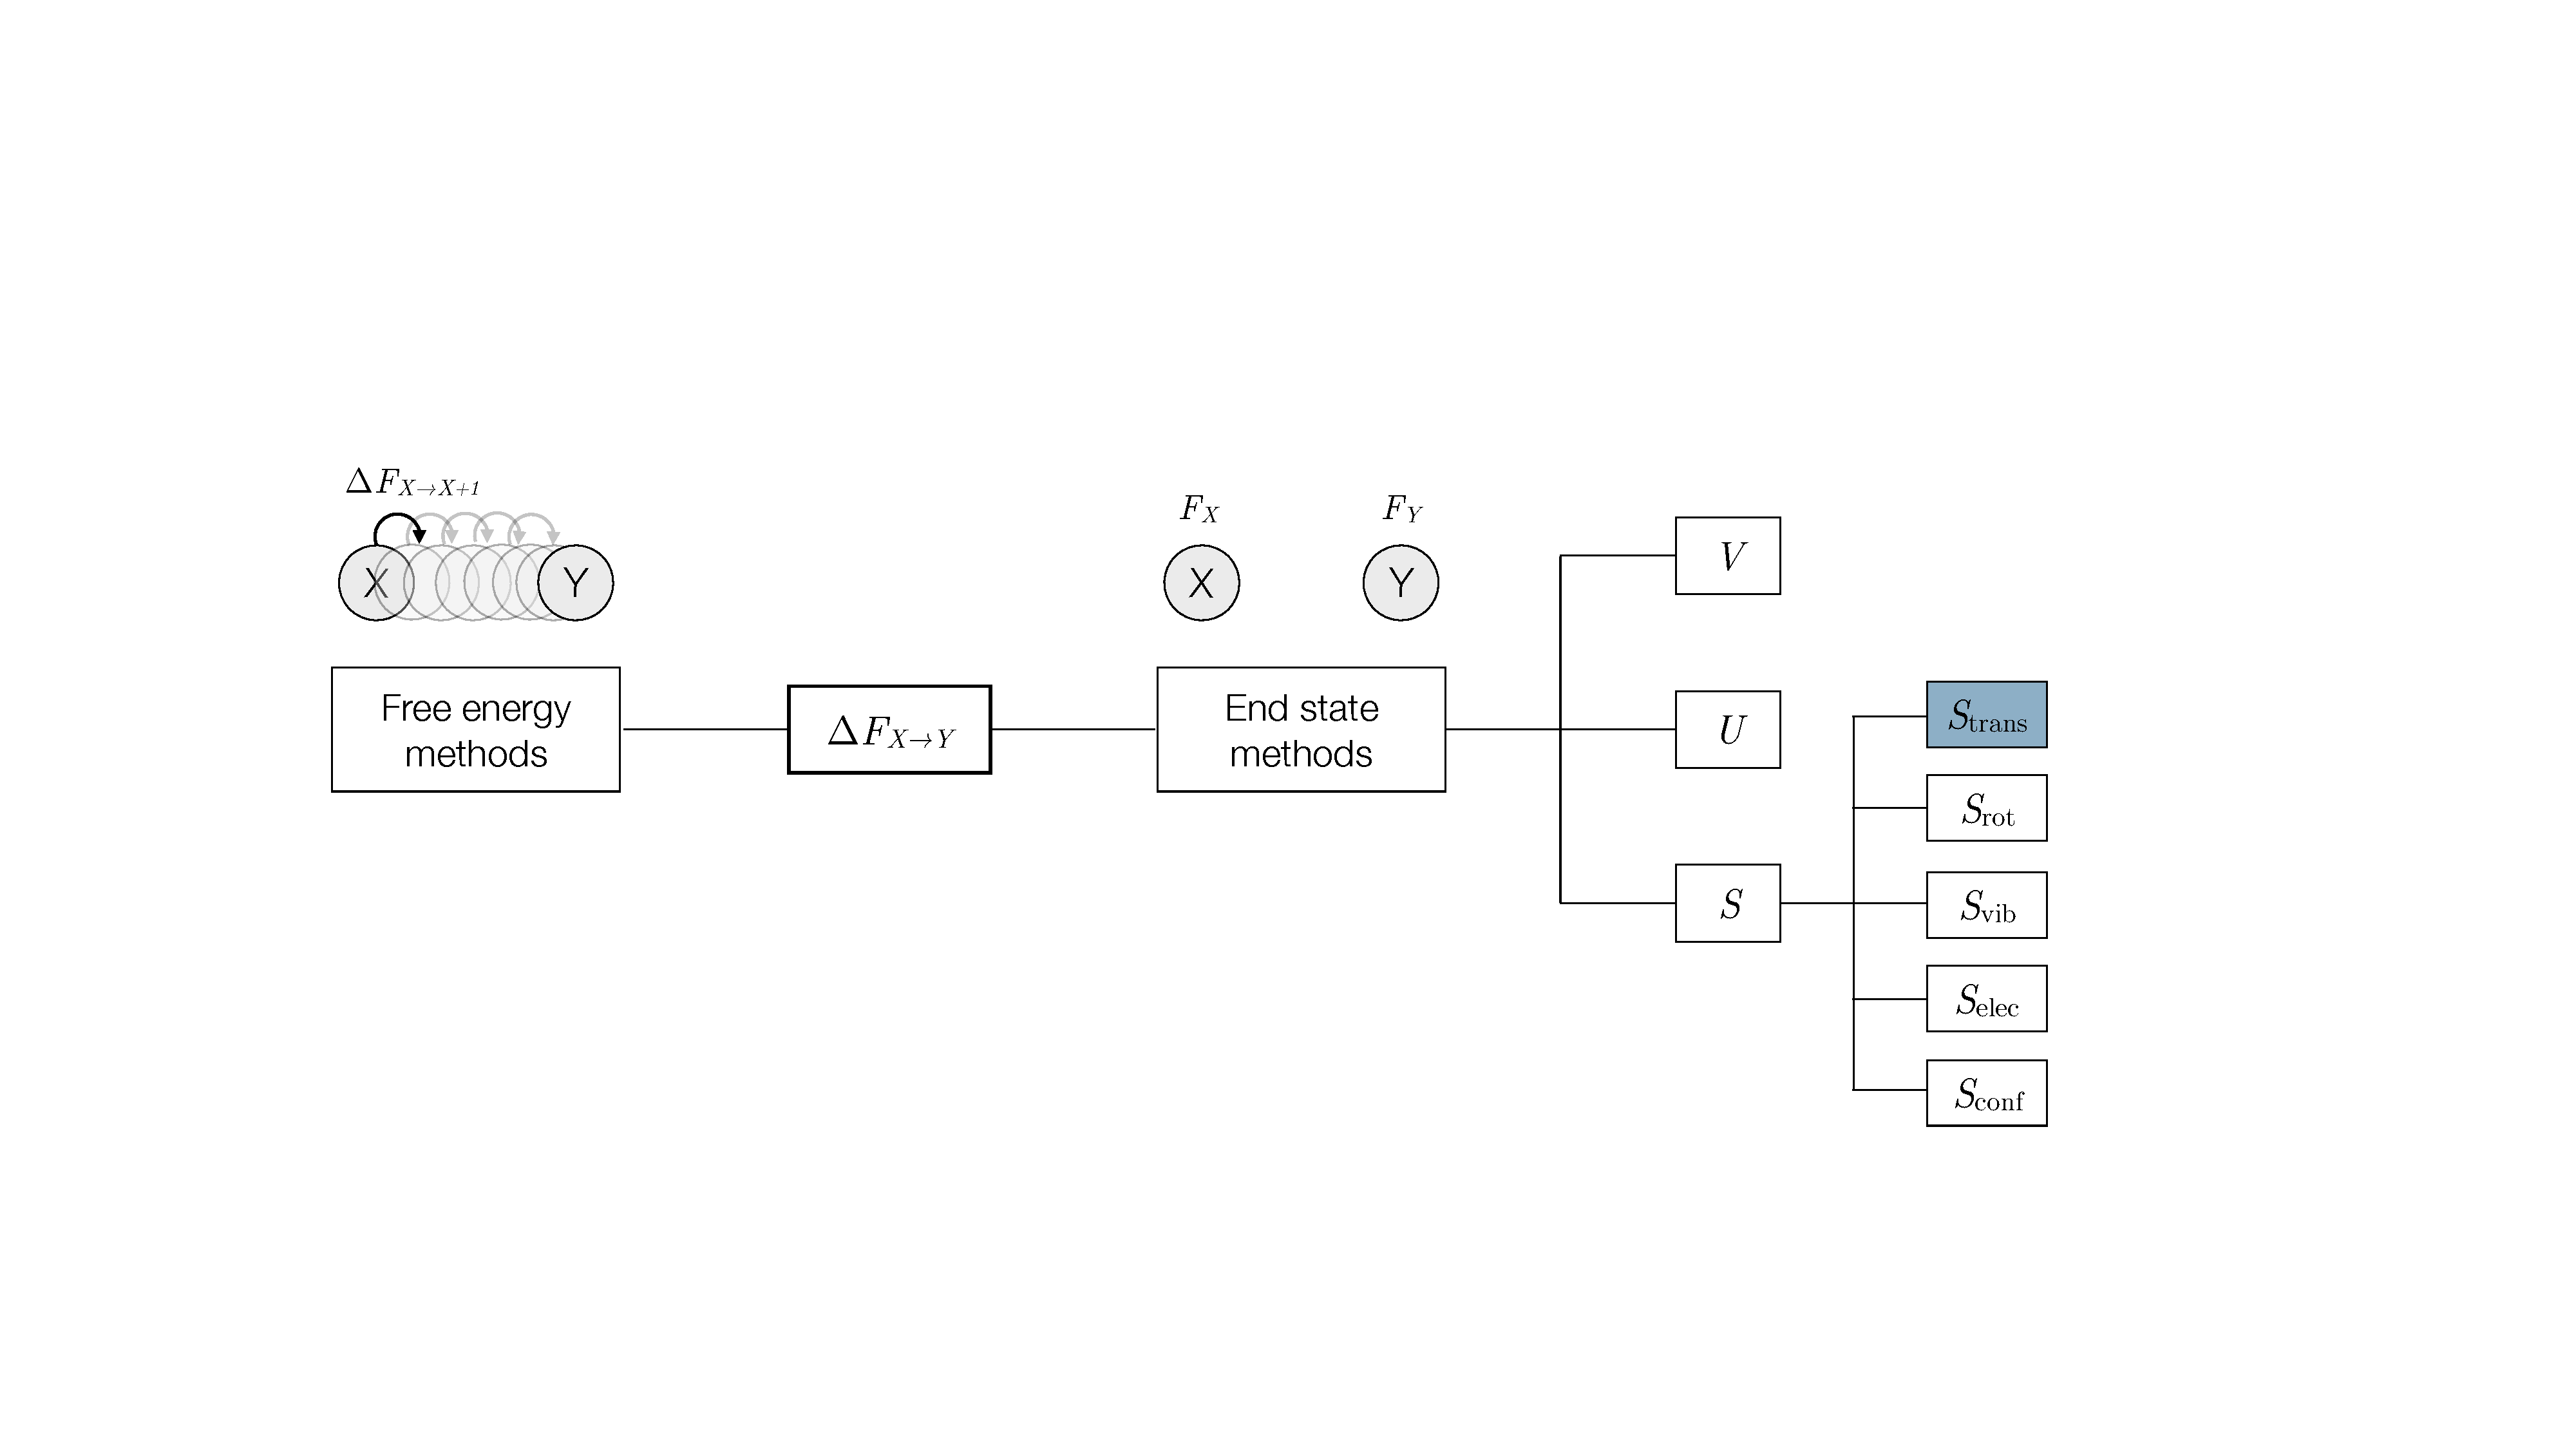
\includegraphics[width=14.5cm]{4/figs/figXA_intro/figXA_intro}
	\vspace{0.4cm}
	\hrule
	\caption{Schematic outline of methods to calculate free energy differences, with the focus of this chapter highlighted in blue.}
	\label{fig::entropy_XA_intro}
\end{figure}

Depending on the end points of the  system and process, the entropic components may cancel and the entropy difference (approximately) vanish, e.g. in unimolecular transformations. However, in an intermolecular chemical process within an environment (e.g. solvent/supramolecular catalyst),
\begin{equation}
\text{A} + \text{B} \xrightarrow{\text{env.}} \text{AB}
\end{equation}
such a cancellation is not generally observed, as the minimum or transition state complex (AB) has lost translational and rotational degrees of freedom compared to the separated components.\cite{Jensen1999} An interesting case occurs when AB comprises a supramolecular structure, where one component (a guest, A) can translate within the host B (as alluded to in Chapter 3). Of particular importance are binding processes in proteins, which govern the affinity of a drug to its biological target.\cite{Woo2005} While in the context of chemical reactivity, an accurate calculation of entropy is required as the rate is exponential in the difference.

\section{Theory}

Calculating $F$ for a stationary point on a PES with QM is achieved by adding  entropic and other contributions to the 0 K potential energy ($U_\text{0 K}$). As most chemical reactions take place at constant pressure, number of molecules and temperature, the appropriate ensemble is isothermal-isobaric ($NPT$). However, the volume change contribution ($P\Delta V$) to the Gibbs free energy is negligible for processes in the condensed phase, including small molecule\footnote{For example, the expt. \cite{Lateef1969} volume of activation for the S$_\text{N}$2 reaction: allyl chloride + H$_2$O $\rightarrow$ allyl alcohol + HCl is $\Delta V^\ddagger = $ ($-11.4 \pm 0.1$) ml mol$^{-1}$, which at $T = 323.4$ K and $P = $1 atm translates to a contribution $P\Delta V = -0.00116$ kJ mol$^{-1}$.} and enzymatic reactions.\cite{Low1975} It is therefore common to predict thermodynamic quantities in the isothermal-isochoric $NVT$ canonical ensemble, where the associated free energy is the Helmholtz energy. From statistical mechanics $A$ is given by,\cite{mcquarrie200}
\begin{equation}
A = -k_B T \ln[Z(N, V, T)]
\label{helmhotlz}
\end{equation}
where $Z$ is the canonical partition function (PF) and $k_B$ is the Boltzmann constant. Were the $NPT$ ensemble to be used the PF would require summation over volume, 
\begin{equation}
Z_P(N, P, T) =  \sum_j Z(N, V_j, T) e^{\beta P V_j}
\end{equation}
where $\beta = 1 / k_B T$. To simplify, with minimal loss in accuracy, thermodynamic quantities are outlined in an $NVT$ ensemble. With electronic structure methods affording $U_{0\text{ K}}$,\footnote{Where the approximate zero-point energy (ZPE) is generally obtained from a harmonic approximation of vibrations and the remaining thermal energy given by standard expressions involving the PF.} the problem broadly reduces to calculating $S$ within the $NVT$ ensemble.\footnote{Note the non-ZPE thermal contributions to the internal energy are small and largely cancel. For example, $\Delta E_\text{internal}^\ddagger = 3.3$ \kcalx for F${}^{-}$+CH${}_3$Cl.} From Eq. \ref{helmhotlz} then,

\begin{equation}
S = k_B T {\Big (} \frac{\partial \ln Z}{\partial T} {\Big )}_{N, V} + k_B \ln(Z)
\label{entropy_Z}
\end{equation}
which only requires the canonical PF for the system.

\subsection{Classical Statistical Mechanics}

Provided the system is sufficiently classical in nature (hot/massive), with negligible nuclear quantum effects and exclusively ground electronic states, the PF may be calculated classically. Classical PFs are integrals over all possible positions and momenta of the particles described by the canonical positions ($\boldsymbol{x}$) and momenta ($\boldsymbol{p}$),\cite{mcquarrie200}

\begin{equation}
	Z = \frac{1}{h^{3}}\int\int e^{-\beta \mathcal{H}(\boldsymbol{p}, \boldsymbol{x})} \; d\boldsymbol{p}^{3} d\boldsymbol{x}^{3}.
	\label{Z_classical}
\end{equation}

For a classical Hamiltonian of the form $\mathcal{H}(x, p) = p^2/2m + V(x)$ momentum may be integrated out to give a purely configurational integral, which -- with sufficient accuracy and sampling -- provides access to all thermodynamic quantities of the system. In principle, calculating $Z$ with classical MD is conceivable, as all possible particle positions and velocities are sampled as $t \rightarrow \infty$. However, in conventional $NVT$ MD simulations the configurational space is already weighted by a Boltzmann factor, reducing the sampling of high-energy regions. Furthermore, regions of the potential energy landscape separated by large energy barriers will rarely be explored. Trying to numerically evaluate Eqn. \eqref{Z_classical} directly by integrating over $\boldsymbol{x}$ explicitly fails for all but the most simple systems ($N \ll 10$) due to the exponential scaling ($3^{N}$) of the configurational space for $N$ particles.



\subsection{Quantum Statistical Mechanics}

The canonical quantum PF is given by,
\begin{equation}
Z = \text{tr}[e^{-\beta \hat{H}}]  = \sum_i g_i \, e^{-\beta E_i}
\label{caonical_pf}
\end{equation}
where $g_i$ is the degeneracy of the $i$'th level with energy $E_i$. Unfortunately, for a macroscopically large chemical system, with $O(10^{23})$ particles, the problem is intractable. Even if all the eigenvalues of the system could be obtained, the sum is impractical to calculate. Indeed, even calculating $Z$ for a particle in an infinite cubic well is challenging and usually approximated by an integral (Eqn. \ref{equation::z_pib_integral}).

To progress, the complexity must be reduced from considering $10^{23}$ particles to just a few. Therefore, the system is assumed to be homogeneous and can be divided into $n$ identical and non-interacting copies to give,
\begin{equation}
Z = \frac{1}{n!} {\Big (} \sum_j g_j \, e^{-\beta E_j} {\Big )}^n \quad := \quad \frac{z^n}{n!}
\label{Z_partion_q}
\end{equation}

where $z$ is the canonical PF of the sub-system and the $n!$ factor corrects for the indistinguishability of the sub-systems. The sum over $j$ now enumerates over all the eigenstates of the subsystem. Despite the system now containing $10^2$--$10^4$ particles it still requires diagonalising a large system and is generally intractable.

A further simplification is therefore required; $z$ is assumed to be factorisable into translational, rotational, vibrational, electronic and conformational contributions for each component in the subsystem i.e. a complete decoupling of molecular motion (\figurename{ \ref{fig::entropy_X1}}),
\begin{equation}
z = \prod_{\text{molecules}} z_\text{trans} \cdot z_\text{rot} \cdot z_\text{vib} \cdot z_\text{elec} \cdot z_\text{conf}
\label{equation::subsystem_pf}
\end{equation}

where approximations to each of these terms are outlined in the following sections.

\begin{figure}[h!]
	\centering
	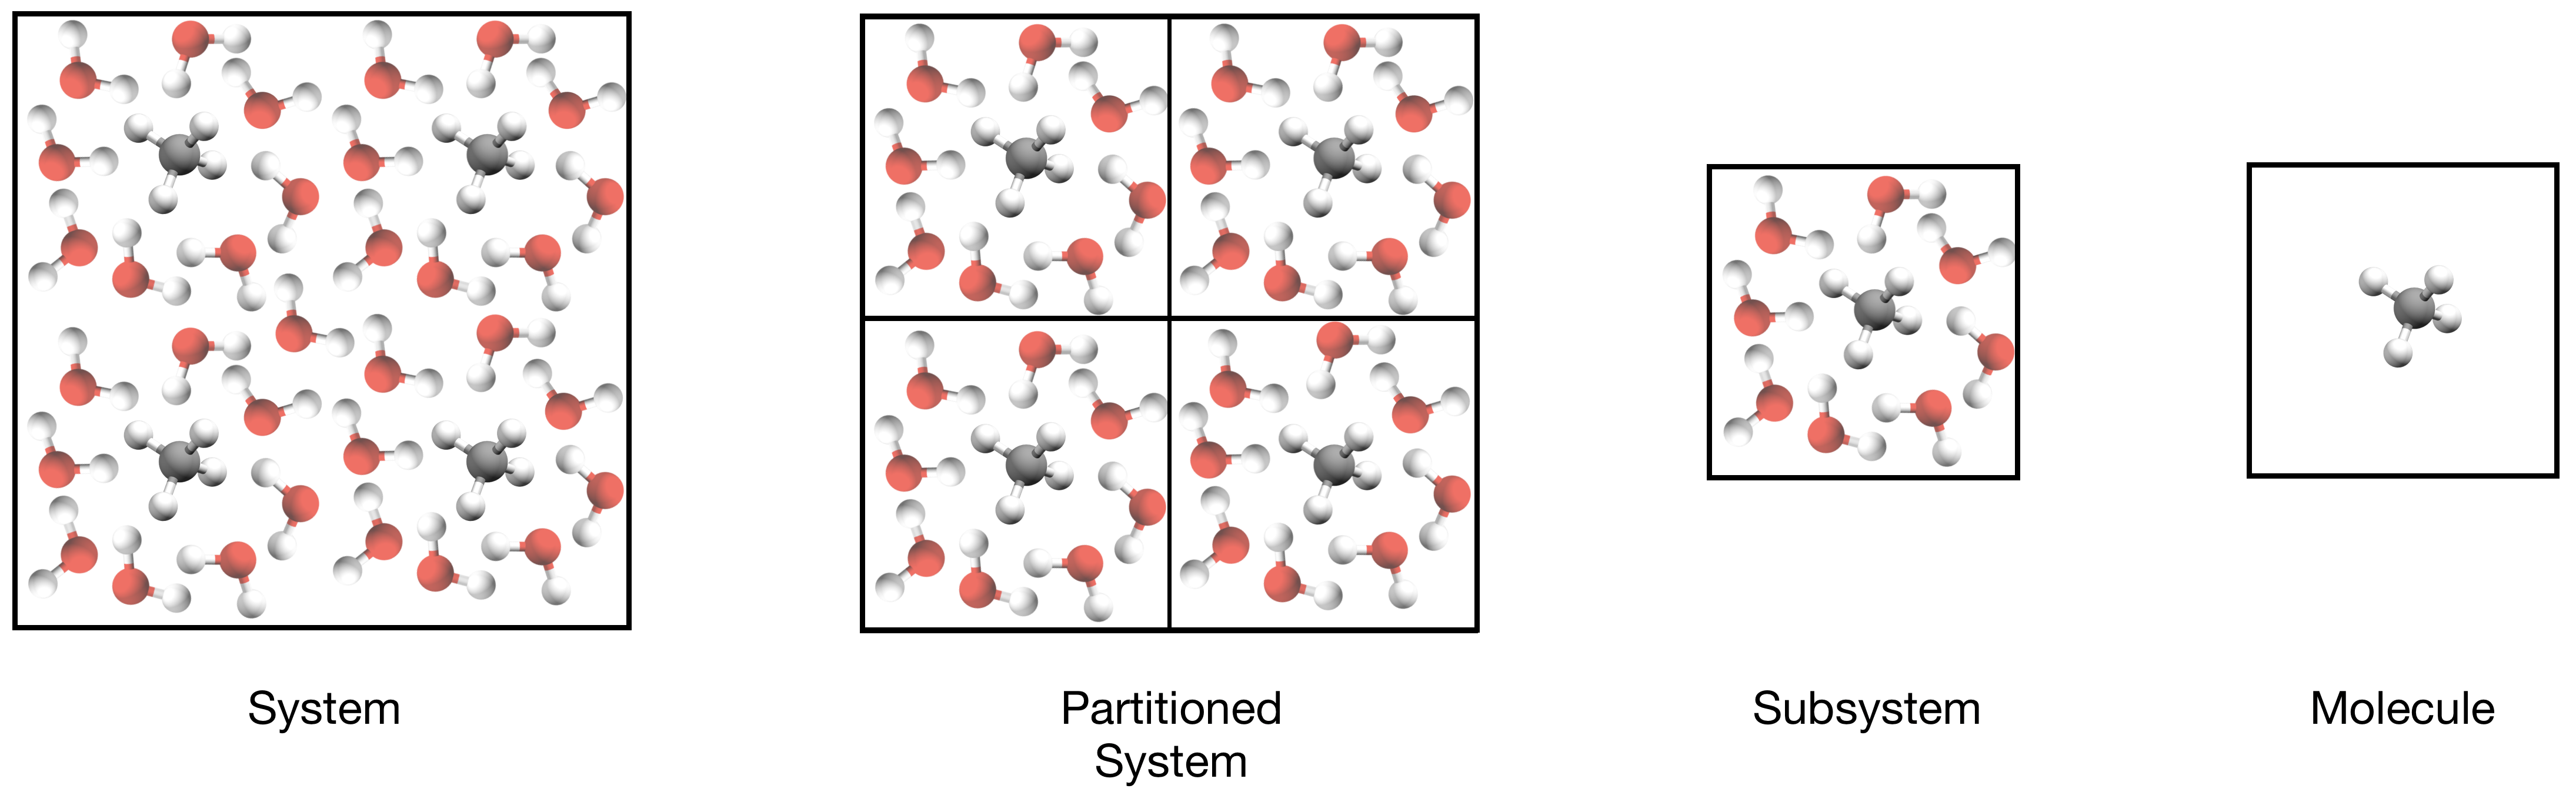
\includegraphics[width=\textwidth]{4/figs/figX1/systems_methane_in_h2o.png}
	\vspace{0.2cm}
	\hrule
	\caption{Example partitioning of a condensed phase molecular system.}
	\label{fig::entropy_X1}
	%systems_methane_in_h2o 
\end{figure}



\subsection{Quantum: Gas Phase}

To calculate the sub-system's PF comprised of a species with a `gas phase' method the environment is completely neglected. Although this places the molecule in vacuum, it is commonly referred to as a `gas phase' method due to its similarity to a low-pressure gas. In this section $z$ [Eqn. \eqref{equation::subsystem_pf}] will refer to a gas phase molecular PF.

If the gap between ground and excited electronic states of the system is large and only the ground state is accessible at room-temperature, thus the electronic component of the molecular PF ($z_\text{elec}$) is assumed to be unity. The conformational component ($z_\text{conf.}$) is often neglected due to a cancellation between states when calculating an energy or entropy difference. Only within the last few years accurate methods to estimate this component have been developed.\cite{Chan2021, grimme2021} This means only the translation, rotation and vibrational states for a single molecule must be approximated.

\subsection{Ideal Gas Method}

Within the ideal gas method (IGM), the molecular PF for a rigid molecule is approximated using analytic expressions for $z_\text{trans}$, $z_\text{rot}$ and $z_\text{vib}$, derived from eigenvalues of a particle in a box (PIB), rigid rotor (RR) and harmonic oscillator (HO) respectively.\cite{mcquarrie200}

\subsubsection{Translation: Particle in a Box}

For a cubic box with sides of length $l$ and a particle of mass $m$ the eigenvalues are,
\begin{equation}
E_n = \frac{\hbar^2 \pi^2}{2ml^2}(n_x^2 + n_y^2 + n_z^2) \qquad :  n_x, n_y, n_z \in \mathbb{N}_{>0}
\end{equation}
from which the PF is then,
\begin{equation}
z_\text{PIB} = \sum_{n_x, n_y, n_z}^\infty \exp{ {\Big \{} -{\beta}\cdot  \frac{\hbar^2 \pi^2}{2ml^2}(n_x^2 + n_y^2 + n_z^2)}{\Big \}} \approx  {\Big (} \frac{2\pi m k_B T}{h^2} {\Big )}^{3/2} V 
\label{equation::z_pib_integral}
\end{equation}
using an integral approximation to the sum.\footnote{The approximation is reasonable in $\ln(q)$, with a $<$1\% error in  $\ln(z_\text{PIB}^\text{sum})/\ln(z_\text{PIB}^\text{integral})$ for a water molecule at 298 K in a cubic box with side length $>$4 \AA. Bound evaluated numerically by summation up to $n_\text{max} = 200$, which is converged with respect to single precision in \emph{numpy}.}

% ----------------------------- numpy to calculate the error ----------------------
%import numpy as np
%
%m = 18 * 1.66053906660E-27       # 1 amu in kg
%kb = 1.380649E-23           # J K-1
%T = 298                       # K
%h = 6.62607004E-34            # J s
%beta = 1.0 / (kb * T)
%max_n = 200
%nx, ny, nz = np.meshgrid(np.arange(0, max_n),
%np.arange(0, max_n),
%np.arange(0, max_n),
%indexing='ij')
%for l_ang in np.linspace(10, 1, num=10):
%l = l_ang*10**(-10)
%q_sum = np.sum(np.exp(-(beta*h**2 /
%(8.0*m*l**2))
%* (nx**2 + ny**2 + nz**2)))
%q_integral = ((2.0*np.pi*m*kb*T)/(h**2))**1.5*l**3
%print(100*(np.log(q_sum) - np.log(q_integral))/np.log(q_sum),
%f'l = {l_ang} Å')

The effective volume ($V$) available is chosen based on the standard state at which the entropy, and so free energy, are required.\cite{Zhou2009} For gases this is usually taken to be the volume available to an ideal gas at 1 atm ($V_\text{1 atm} = 1 / \beta p= 40605$ \AA${}^3$) and 1 mol dm${}^{-3}$ for solutions ($V_\text{1 M} = 1/ C =  1661$ \AA${}^3$). For gas phase reactions this approximation is excellent -- delivering quantitative accuracy to experiment in a selection of reaction rates.\cite{Shan2019} However, in solution using an effective volume appropriate for an ideal gas is controversial, with `free volume' theories proposed to correct for the potential overestimation of the effective volume and so entropy.\cite{Amzel1997} These strategies will be discussed in the context of a new method outlined below.

\subsubsection{Rotation: Rigid Rotor}

The standard IGM expression for the rotational PF is outlined below for completeness and is generally accurate for most molecules in the gas phase as it does not significantly contribute to the entropy.


%assuming rigid rotation are presented elsewhere.\cite{mcquarrie200} Again an integral approximation is made to evaluate the sum, and is accurate for most molecules in the gas phase.

% ------------------------------- Unimportant for the story -------------------------------
%\iffalse

Evaluating the rigid rotor PF requires the species' symmetry, as $z_\text{rot}$ differs for symmetric, spherical and asymmetric tops (amongst others). Using a spherical top to simplify the calculation, with moment of inertia  $I$ has eigenvalues,
\begin{equation}
E_J = \frac{\hbar^2}{2I} J(J+1) \qquad: J \in \mathbb{N}_{>0}
\end{equation}
with degeneracy $g_J = (2J + 1)^2$. The PF is evaluated at the continuum limit noting that large $J$ will contribute most to the integrand (provided $\hbar^2/2I\beta \ll 1$) so $J + 1 \sim J$,
\begin{equation}
z_\text{rot} = \sum_{J}^\infty (2J + 1)^2\exp{ {\Big \{} -{\beta}\cdot  \frac{\hbar^2}{2I}J(J+1)}{\Big \}} \approx \sqrt{\pi} {\Big (} \frac{2I k_b T}{\hbar^2} {\Big )}^{3/2}
\label{z_rot_spherical_top}
\end{equation}
Generalisation of Eqn. \eqref{z_rot_spherical_top} to a molecule with unequal moments of inertia ($I_x \neq I_y \neq I_z$) is assumed to be possible and, when divided by a symmetry number $\sigma_r$, is given by,
\begin{equation}
z_\text{rot} = \frac{\sqrt{\pi}}{\sigma_r} \cdot \sqrt{\frac{ (k_B T)^3}{B_x B_y B_z}}
\end{equation}
where the rotational constants are of the form $B_k = \hbar^2/2 I_k $ where $I_k$ is the moment of inertia in the $k$ axis.

%and the moments of inertia are calculated using;
%\begin{equation}
%I_x = \sum_{i}^{\text{atoms}} m_i (y_i^2 + z_i^2) \quad;\quad I_y = \sum_\text{i}^{\text{atoms}} m_i (x_i^2 + z_i^2) \quad ; \quad I_z = \sum_\text{i}^{\text{atoms}} m_i (x_i^2 + y_i^2) 
%\end{equation}

%where $x_i, y_i, z_i$ are displacements of atom $i$ from the centre of mass in the Cartesian directions.

%\fi
% -------------------------------------------------------------------------------------------

\subsubsection{Vibrational: Harmonic Oscillator}

By diagonalising the mass-weighted matrix of second derivatives (the Hessian), the normal mode frequencies can be obtained from the eigenvalues, so that the vibrational PF can be obtained as a product over the individual uncoupled harmonic oscillators (HOs). Given for quantum HO,
%By decomposing the vibrational motion into normal modes the Hessian becomes diagonal with the eigenvalues corresponding to independent harmonic frequencies (once mass weighted). The partition function may then be computed from product of the independent HO partition functions for all these modes. From the eigenvalues of a simple harmonic oscillator and summing directly,
\begin{equation}
E_n = \hbar\omega {\Big (} n + \frac{1}{2} {\Big )} \qquad : n \in \mathbb{N}_{\ge 0}
\end{equation}
%\begin{equation}
%\begin{aligned}
%q_\text{HO} &= \sum_{n}^\infty \exp {\Big \{} -{\beta}\cdot  \hbar\omega {\Big (} n + \frac{1}{2} {\Big )} {\Big \}} \\
%&= e^{-\beta\omega\hbar/2}\sum_{n}^\infty e^{  -{\beta}\hbar\omega n} \\
%&= e^{-\beta\omega\hbar/2} \cdot  \frac{1}{1 - e^{  -{\beta}\hbar\omega}} \\
%&= \frac{e^{-h\nu / 2 k_B T}}{1 - e^{-h\nu / k_B T} }
%\end{aligned}
%\end{equation}
then,
\begin{equation}
	z_\text{HO} = \sum_{n}^\infty \exp {\Big \{} -{\beta}\cdot  \hbar\omega {\Big (} n + \frac{1}{2} {\Big )} {\Big \}}  = \frac{e^{-h\nu / 2 k_B T}}{1 - e^{-h\nu / k_B T} }
\end{equation}
where $\nu = \omega / 2\pi$. The total molecular PF is then given by a product over normal modes as,
\begin{equation}
z_\text{vib} = \prod_j^{N} \frac{e^{-h\nu_j / 2 k_B T}}{1 - e^{-h\nu_j / k_B T} } \qquad : \qquad  N = \begin{cases}
	3 n_\text{atoms} - 5 \quad\text{if linear} \\
	3 n_\text{atoms} - 6 \quad\text{otherwise} \\
 \end{cases}
\label{z_ho}
\end{equation}

This simple expression is, however, limited in the low-frequency regime where $\nu \sim 10 \text{ cm}^{-1}$, which are prevalent in molecules with more than a few atoms. These may correspond to dihedral rotations or translations and are not well approximated by a harmonic well.\footnote{Indeed $\lim_{\nu \rightarrow 0^+} (z_{j, \text{vib}})= \infty$ which affords an unphysical divergence in the entropy for a molecule.} Furthermore, these low frequency modes (LFMs) are subject to numerical noise and with a poorly converged geometry or an imprecise Hessian and can become imaginary.

To counter this deficiency Truhlar suggested that a \emph{post hoc} shift should be applied to all harmonic frequencies below a certain threshold ($\nu_0$, i.e. $\nu = \max(\nu, \nu_0)$) designated as LFMs.\cite{Ribeiro2011} However, the choice of cut-off is not uniquely defined and -- as Harvey and co-workers found -- can lead to $\Delta G$ differences in excess of 5 \kcal.\cite{Liu2017} 

Grimme and co-workers proposed an alternative LFM treatment that improved the agreement between theory and experiment for guest binding.\cite{Grimme2012} By treating LFMs as free rotors with average moment of inertia, then interpolating between the free rotor and HO regimes $z_\text{vib}$ is scaled down. However, parameters must be set once again, this time governing the form of the weighting function. 


\subsection{Alternative Methods}

While the IGM is commonplace in electronic structure theory codes for calculating the thermal (enthalpic and entropic) contributions to the absolute free energy, it is not without limitations. Specifically, the translational component of the entropy is often considered to be overestimated for molecules in solution.\cite{Gilson2010} Indeed, various scaling factors have been proposed in order to improve computational accuracy with varying levels of justification. For example, neglecting both the translational and rotational components,\cite{Sumimoto2004} removing the translational component,\cite{Tanaka2011} scaling by 0.5 and inverting the sign,\cite{Deubel2006} scaling by 0.5,\cite{Li2016} and scaling by 2/3.\cite{DiTommaso2010} In addition to empirical scalings, recent work by Garza\cite{Garza2019} makes use of an effective volume within $z_\text{PIB}$ given by,
\begin{equation}
V_\text{Garza} = N_c v_c
\end{equation}
where $N_c$ is the number of available cavities for the solute and $v_c$ the cavity volume within a solvent. The PIB approximation for condensed phase systems is, however, theoretically limited. Molecules are not hard spheres and have a free path in solution $O(1 \text{ \AA})$;\cite{Herman2016} indeed, most empirical forcefields make use of a Lennard-Jones $1/r^{12}$ repulsive term rather than a step function. This may result in a over/under-estimation of the translational entropy depending on the box size.

Other approaches have moved beyond the PIB treatment, to a harmonic oscillator approximation of the explicit translational motion. For example, the method by Henchmen and co-workers treats  translational/rotational and vibrational components by diagonalising the force covariance matrix in a particular reference frame to afford frequencies that are used within a quantum harmonic oscillator expression for the entropy.\cite{Chakravorty2020, Ali2019} A similar method based on QM calculations by Nakai and co-workers, referred to as the `harmonic solvation model' (HSM), treats all normal modes of the solute as vibrations.\cite{Nakai2014} At least superficially this would seem reasonable as in solution a molecule has no free translation, or -- to a lesser extent -- rotation. This method recovers the equipartition limit for the internal energy for translation and rotation as $\nu \rightarrow 0$ cm$^{-1}$ namely,

\begin{equation}
E_\text{trans/rot} = \frac{k_B T}{2} \sum_i^3 \lim\limits_{\nu_i \rightarrow 0} \left[ {\beta\nu_i} {\Big (} \frac{1}{2} + \frac{e^{-\beta\nu_i}}{1-e^{-\beta\nu_i}} {\Big )}\right] = \frac{3}{2} k_B T.
\end{equation} 

Nakai suggested computing the frequencies using an implicit solvent model (CPCM); however, this must be performed numerically as the implicit solvent cavity must remain fixed i.e. not relaxed to accommodate the displaced geometry. Moreover, the numerical frequency calculation must be performed on a structure that has been optimised in the solution phase, thereby increasing the calculation time by hindering geometry convergence. For large systems this method therefore becomes prohibitively expensive.


The same authors reported a variant of this approach in 2018,\cite{Tarumi2018} where the intramolecular vibrational modes are treated within the IGM (rigid-body HSM, RB-HSM). This model was tested on a small set of vaporisation (7) and combustion (5) entropies and performed similarly to the more expensive HSM. Translational and rotational motion are then calculated by diagonalising a 6$\times$6 Hessian matrix consisting of the second derivatives with respect to translation and rotation in the Cartesian directions. For water this treatment results in harmonic frequencies $>$ 70 cm$^{-1}$; however, for 1,2-dichloroethane (DCE) the lowest frequency mode treated harmonically is just 6.4 cm$^{-1}$. For such a small force constant, the harmonic approximation is a poor one, with the associated entropy contribution potentially overestimated.

It is worth noting that in the systems tested by Garza, Henchmen and Nakai the agreement to experiment is excellent in all cases, despite the disparity in methods. Therefore, the question of which method is physically based and so generally applicable remains.

\subsection{Concentration Corrections}

A meaningful comparison to experiment requires comparing free energies that have been obtained at the same (standard) state, which for molecules is usually taken to be 1 M. A correction is then needed to calculate a free energy at the standard state for an unequal simulation volume of,\cite{General2010} 
\begin{equation}
	F^{\standardstate} = F^\text{sim} + k_BT \ln\left(\frac{V^\standardstate}{V^\text{sim}}\right)
\end{equation}
where $F$ is a free energy ($G, A$) and $V^\text{sim}$ the volume used for the simulation. 

In calculating the translational entropy within a defined cavity the solute concentration is far from the 1 M standard. While solvent dependent, it should be of the same order of magnitude as the solute volume. For example, considering a methane-in-water system, which is close to ideal spherical case, the molecular volume is $\sim 30$ \AA$^3$\cite{Zhao2003} thus to correct into 1 M (an effective volume of 1661 \AA$^3$) an absolute upper bound is 2.4 \kcal. 
%8.3145*298.15*ln(1661/30)/1000/4.184
Therefore, 2.5 \kcalx provides a useful upper bound on the concentration correction the true `simulation' volume from which the exponential well is obtained is larger than just the molecular volume. In fact, with a molecular volume more representative of those usually studied in solution phase reactions, with a radius $\sim 5$ \AA$\;$  ($\sim 500-700$ \AA$^3$ is common in drug-like molecules\cite{Khanna2009}) the volume correction decreases to just 0.5–-0.7 \kcalx at room temperature. Thus, in all but the smallest solvated molecules, this contribution is small.
\\
It is worth noting that this correction term is distinct from the entropy of mixing, as the maximum $TS_\text{mix} \sim 0.4\;$ \kcal,\footnote{Obtained from the standard statistical mechanics result $\Delta S_\text{mix} = -R(x \ln x + (1-x)\ln(1 - x))$ for a two component system one of which has mole fraction $x$.}  and thus generally negligible at ambient temperature or below.


\section{Limitations of the IGM and Harmonic Approximation}
\subsection{Model Systems}

While the quantum PF and thus entropy of a HO diverges as the frequency becomes small,\footnote{As it should with the Hamiltonian becoming that of a free particle, with $S_\text{HO}^\text{quantum} \sim k_B\ln(k_B T/h\nu) : \nu \ll 1$, but is clearly unphysical for a molecule.} a classical treatment affords another an even greater deficiency. Specifically, the classical HO entropy is,
\begin{equation}
S^\text{classical}_\text{HO} = k_B \ln\left(\frac{k_BT\text{e}}{h\nu}\right)
\end{equation}
which becomes negative and unphysical as $k_BT \sim h\nu$ (\figurename{ \ref{s_vs_nu}a}). Plotting the classical and quantum entropies as a function of the oscillator frequency, the classical entropy becomes negative at a frequency of just 540 cm$^{-1}$. If the HO is used as an approximation for a bond (as for stretches in most force fields) the entropy should certainly be positive. Although this behaviour has been noted previously, and a correction proposed,\cite{Schlitter1993} it is striking. Significant care must then be taken when estimating absolute or relative entropy differences with a classical method.

\begin{figure*}[h!]
	
	\centering
	\begin{subfigure}[b]{0.49\textwidth}
		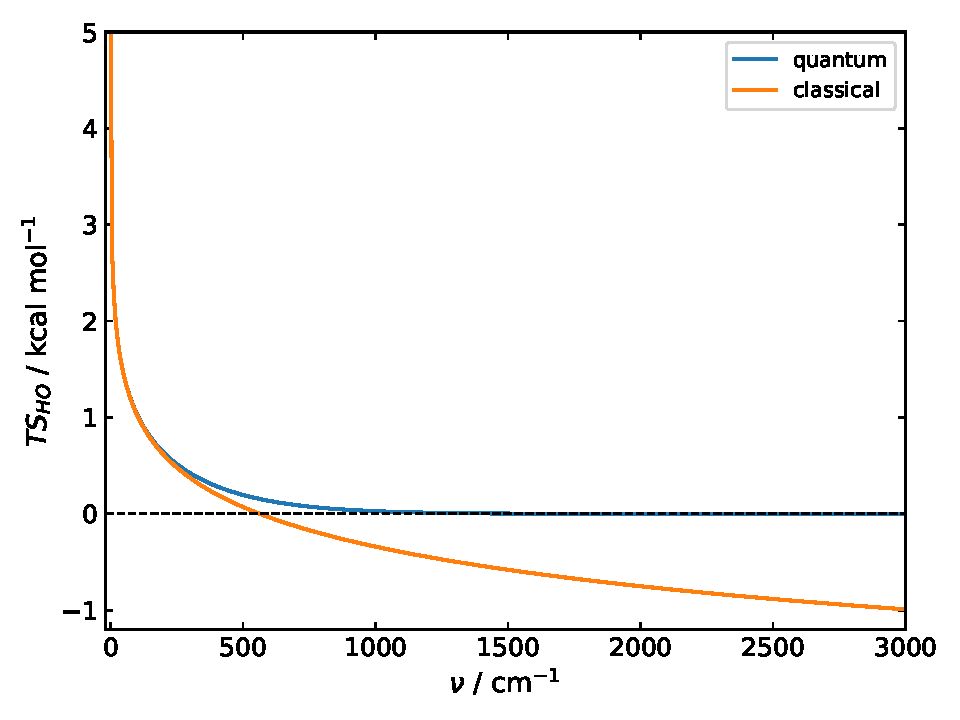
\includegraphics[width=8.2cm]{4/figs/fig_s_vs_nu/s_vs_n.pdf}
			\caption{}
	\end{subfigure}
	\hfill
	\begin{subfigure}[b]{0.49\textwidth}
		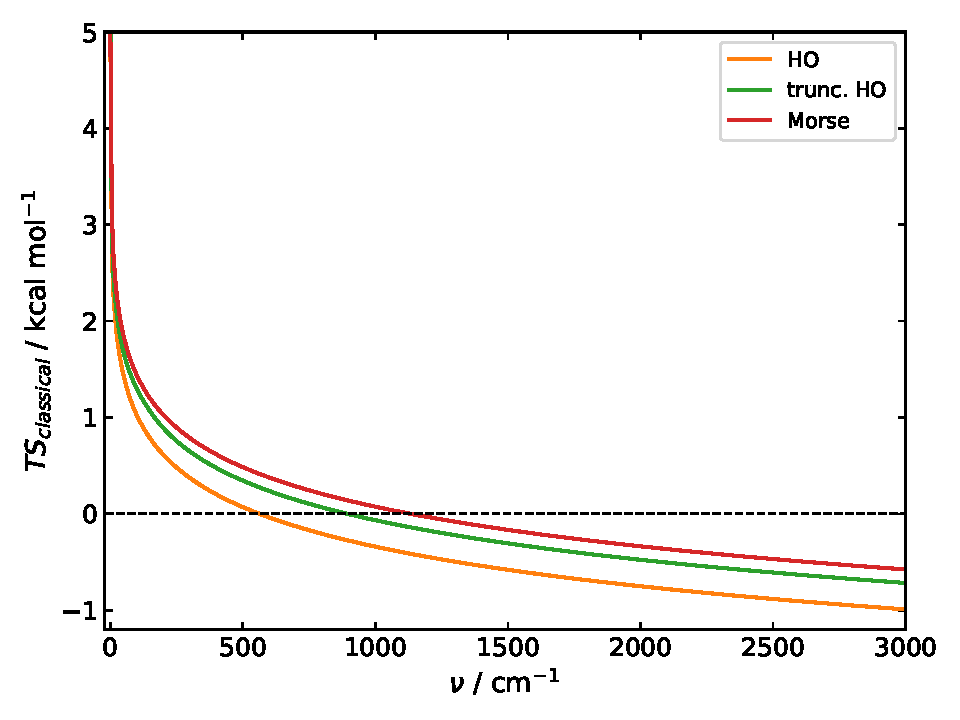
\includegraphics[width=8.2cm]{4/figs/fig_s_vs_nu/s_vs_nu_trunc_morse.pdf}
		\caption{}
	\end{subfigure}
	\vspace{0.2cm}
	\hrule
	\caption{(a) Molar entropy ($S$) of non-interacting quantum and classical harmonic oscillators vs oscillator frequency at $T = 298.15 $ K. (b) Molar entropy ($S$) of non-interacting oscillators vs oscillator frequency at $T = 298.15 $ K. $S_\text{Morse}$ was calculated by evaluating the partition function numerically over [$-\frac{1}{a}\ln(2)$, 5] \AA, at $10^4$ points with a trapezium integrator (converged quantities). $D_e$  fixed at 400 kJ mol$^{-1}$ and $a$ modified according to the harmonic frequency. $\partial Z / \partial T$ calculated using a finite difference ($\delta T = 1 \times10^{-8}$ K).  $r_e = 1$ \AA.}
	\label{s_vs_nu}
\end{figure*}

In calculating the PF for a classical HO the integral runs over an unphysical region beyond where the atoms pass through each other at $r = 0$, where $r$ is the internuclear separation and $r_e$ its equilibrium value. Two potentials with more realistic behaviour are that of a truncated HO,

\begin{equation}
	V(r) = \begin{cases}
		\infty \qquad\qquad\;\;\;\; r \le 0 \\
		k (r - r_e)^2 \qquad r > 0
	\end{cases}
\end{equation}

and a Morse oscillator,
\begin{equation}
	V(r) = D_e(1 - \exp\left[(-a(r- r_e))\right])^2.
\end{equation}
The truncated HO captures the region where the internuclear separation becomes negative, but fails to describe the bond dissociation. The Morse oscillator has the opposite limitations describing the dissociation well but without $V \rightarrow \infty$ as $r \rightarrow 0$.\footnote{In fact, this region is largely captured correctly in calculation of the PF as the particle must be bound (to ensure convergence of the integral) thus $E < D_e$ and so $x > -\frac{1}{a}\ln(2)$ which is greater than $ -r_e$ for $\omega > 630$ cm$^{-1}$} 



% --------------------------------- Dull and simple --------------------
\iffalse
\begin{figure*}[h]
	\centering
	\begin{subfigure}[t]{0.5\textwidth}
		\centering
		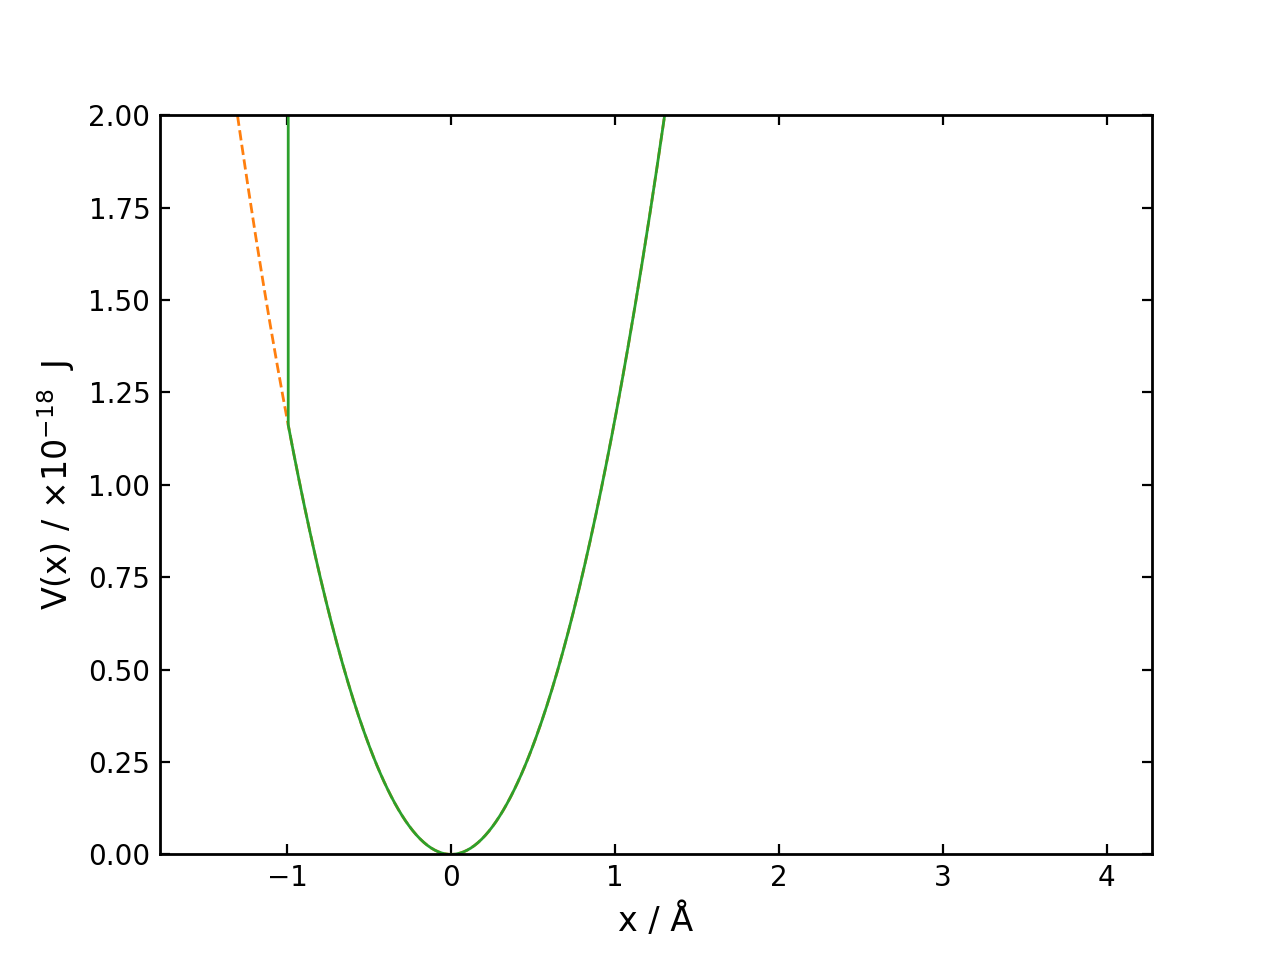
\includegraphics[height=6.5cm]{4/figs/v_vs_x_trunc_ho}
		\caption{}
	\end{subfigure}%
	~ 
	\begin{subfigure}[t]{0.5\textwidth}
		\centering
		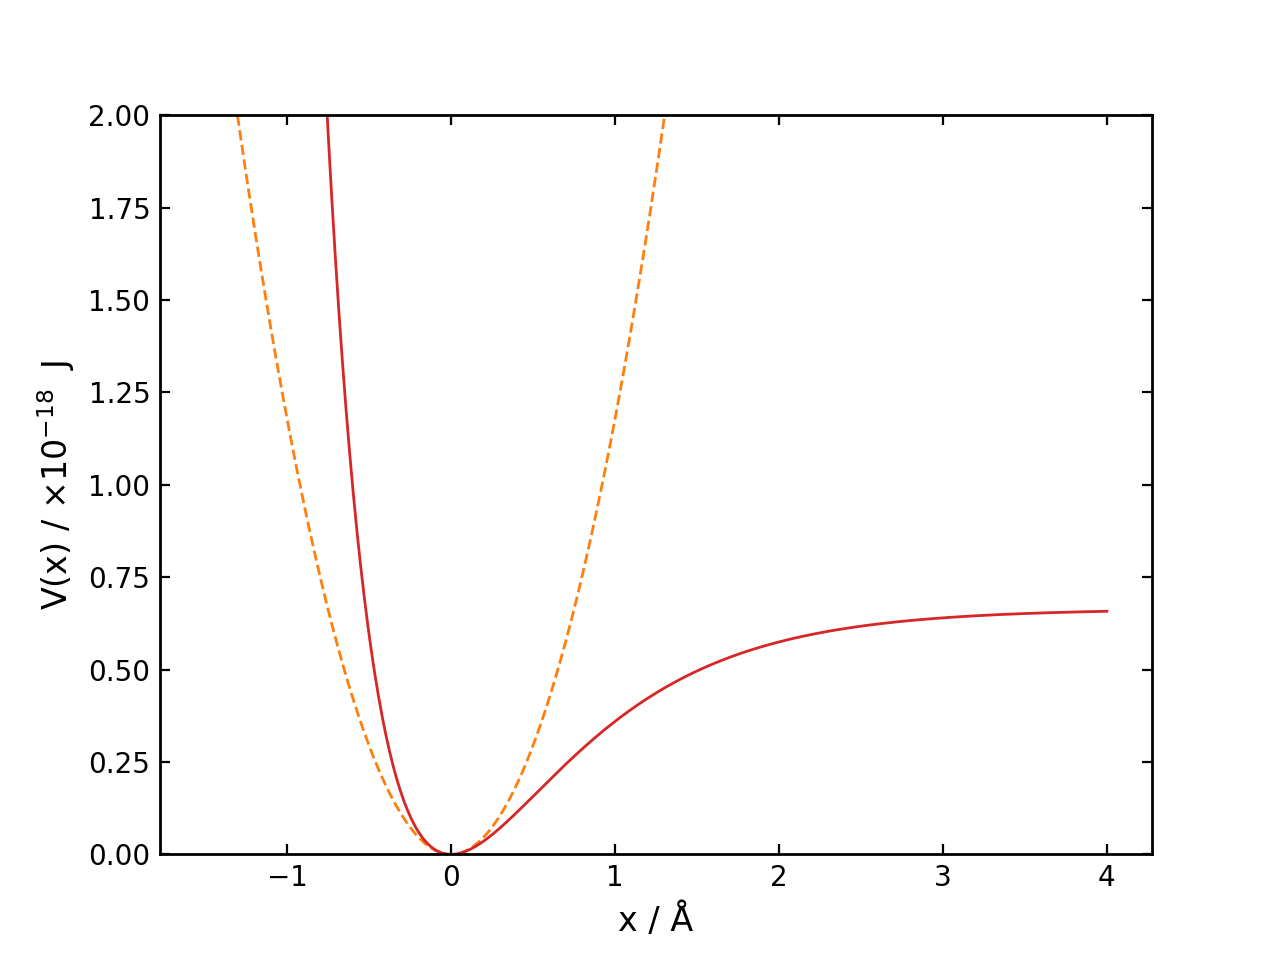
\includegraphics[height=6.5cm]{4/figs/v_vs_x_morse}
		\caption{}
	\end{subfigure}
	\vspace{0.2cm}
	\hrule
	\caption{Potential energy as a function of displacement from equilibrium $x = r - r_e$ for (a) a truncated HO and (b) a Morse oscillator, $V(x) = D_e(1 - e^{-ax})^2$. $r_e = 1$ \AA, $\nu = 2000 \;\text{cm}^{-1}$, $D_e = 400$ kJ mol$^{-1}$, $m = 1$ amu.}
	\label{v_vs_x_morse_trunc}
\end{figure*}
\fi
% -------------------------------------------------------------------



Despite these improvements over the HO potential, the resulting entropy still becomes negative for an oscillator with a frequency above $1000$ cm$^{-1}$ (\figurename{ \ref{s_vs_nu}}). Derivations of truncated HO and Morse partition functions are presented in the Appendix \ref{section::appendix_igm_partition_functions}.

%\begin{figure}[h!]
%	\centering
%	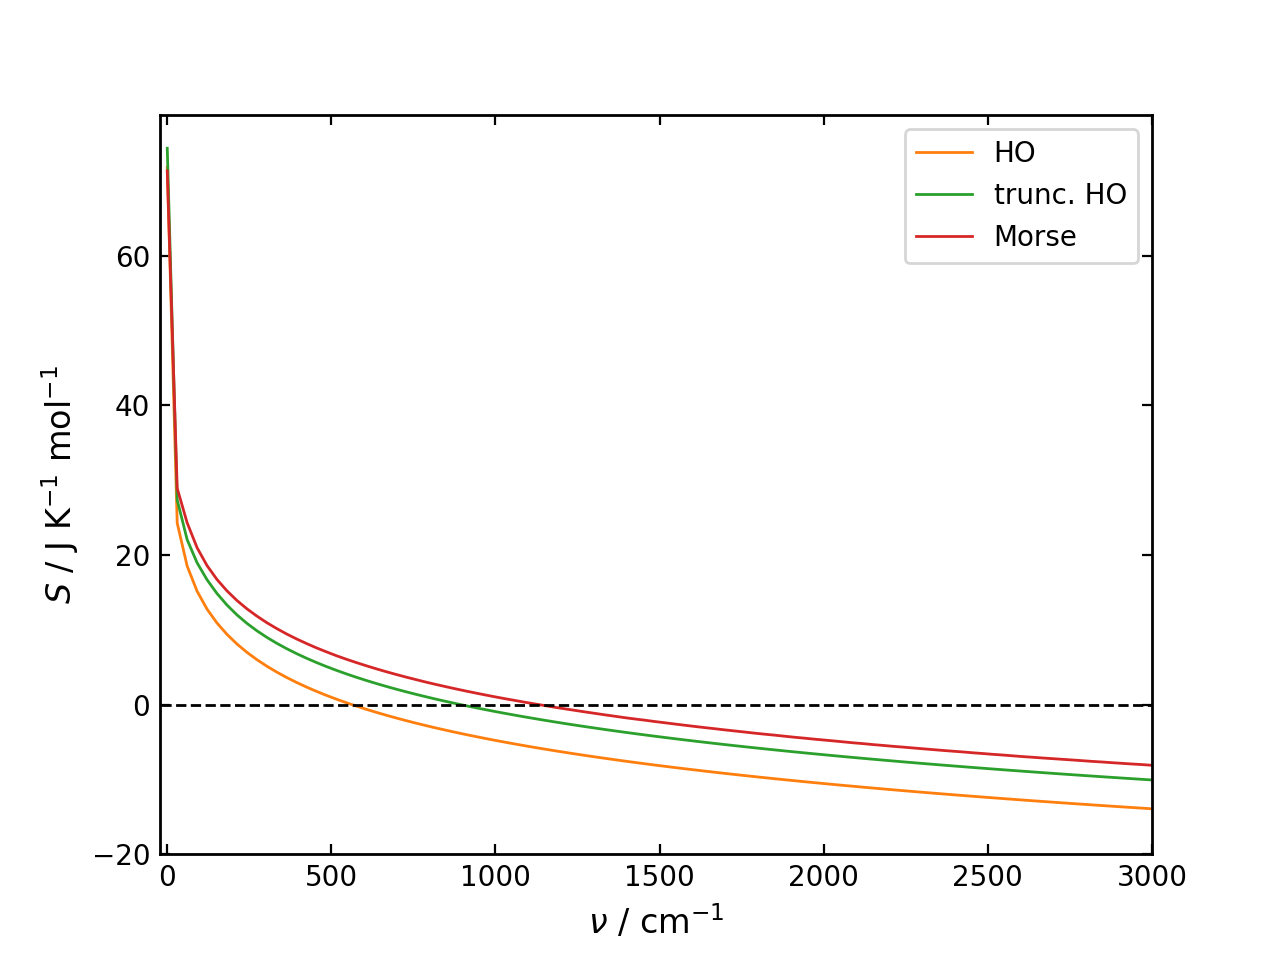
\includegraphics[width=11cm]{4/figs/s_vs_nu_trunc_morse}
%	\vspace{0.2cm}
%	\hrule
%	\caption{).}
%	\label{s_vs_nu_trunc_morse}
%\end{figure}

These results imply that for systems with \emph{high} frequency oscillators ($> 500$ cm$^{-1}$) any classical method for calculating thermodynamic quantities will be incorrect. This includes notable methods based on the covariance matrix from Karplus\cite{Karplus1981} and the interaction energy from Duan\cite{Duan2016}. The latter experiencing a smaller deficiency, provided terms in the interaction energy do not include any \emph{high} frequency oscillators. 

This result implies that all molecular vibrations ($\gtrsim 200\text{ cm}^{-1}$) in a solute-solvent system must be treated quantum mechanically. This includes both bond stretches and bends; as for example, an aliphatic C--H stretch has $\nu \sim 2900$ cm$^{-1}$ and bend $\nu \sim 1350$ cm$^{-1}$.\cite{Coates2006} As such, the deficiency in computing the entropy classically cannot be relieved by simply fixing bond lengths using e.g. the LINCS algorithm.\cite{Hess1998} Rather, all angles and bond lengths must be fixed or treated with QM to ensure only oscillators where $h\nu \ll k_B T$ contribute. 


\subsection{Water-in-Water}

Limitations of the IGM become particularly apparent when considering cluster-continuum solvation of a solvent molecule. Taking water as a model system and considering the identity reaction,
\[(\text{H}_2\text{O})_{n, (\text{aq})} \rightarrow (\text{H}_2\text{O})_{n - 1, (\text{aq})} + \text{H}_2\text{O}_{(\text{aq})}
\]
the free energy and entropy change is zero. However, when calculated using the IGM the free energy change is exergonic by up to 9 \kcal (\figurename{ \ref{fig::entropy_X2}}) for $n=8$. Unfortunately, implicit solvent models do not decompose the solvation free energy into entropic and enthalpic components thus $\Delta S$ does not include $\Delta\Delta S_\text{solv}$. Nevertheless, irrespective of the approximation made within the IGM, and solvent model utilised, the free energy of dissociating a water octamer into a septamer and monomer is incorrect.\footnote{Note that the electronic potential energies calculated at DLPNO-CCSD(T)//def2-TZVPP are not counterpoise corrected; however, recalculation with a more complete QZVPP basis afforded only a small difference ($\Delta E_\text{QZ} - \Delta E_\text{TZ} = -0.3$ \kcal).} The dominant contribution to this energy is the $-T\Delta S$ term, which is approximately $ -10\;$\kcalx (\figurename{ \ref{fig::entropy_X2}, right}). This effect is exacerbated when the cluster is fully dissociated, with the corresponding identity reaction exergonic by 60 \kcal. 


\begin{figure}[h!]
	\centering
	\vspace{1.0cm}
	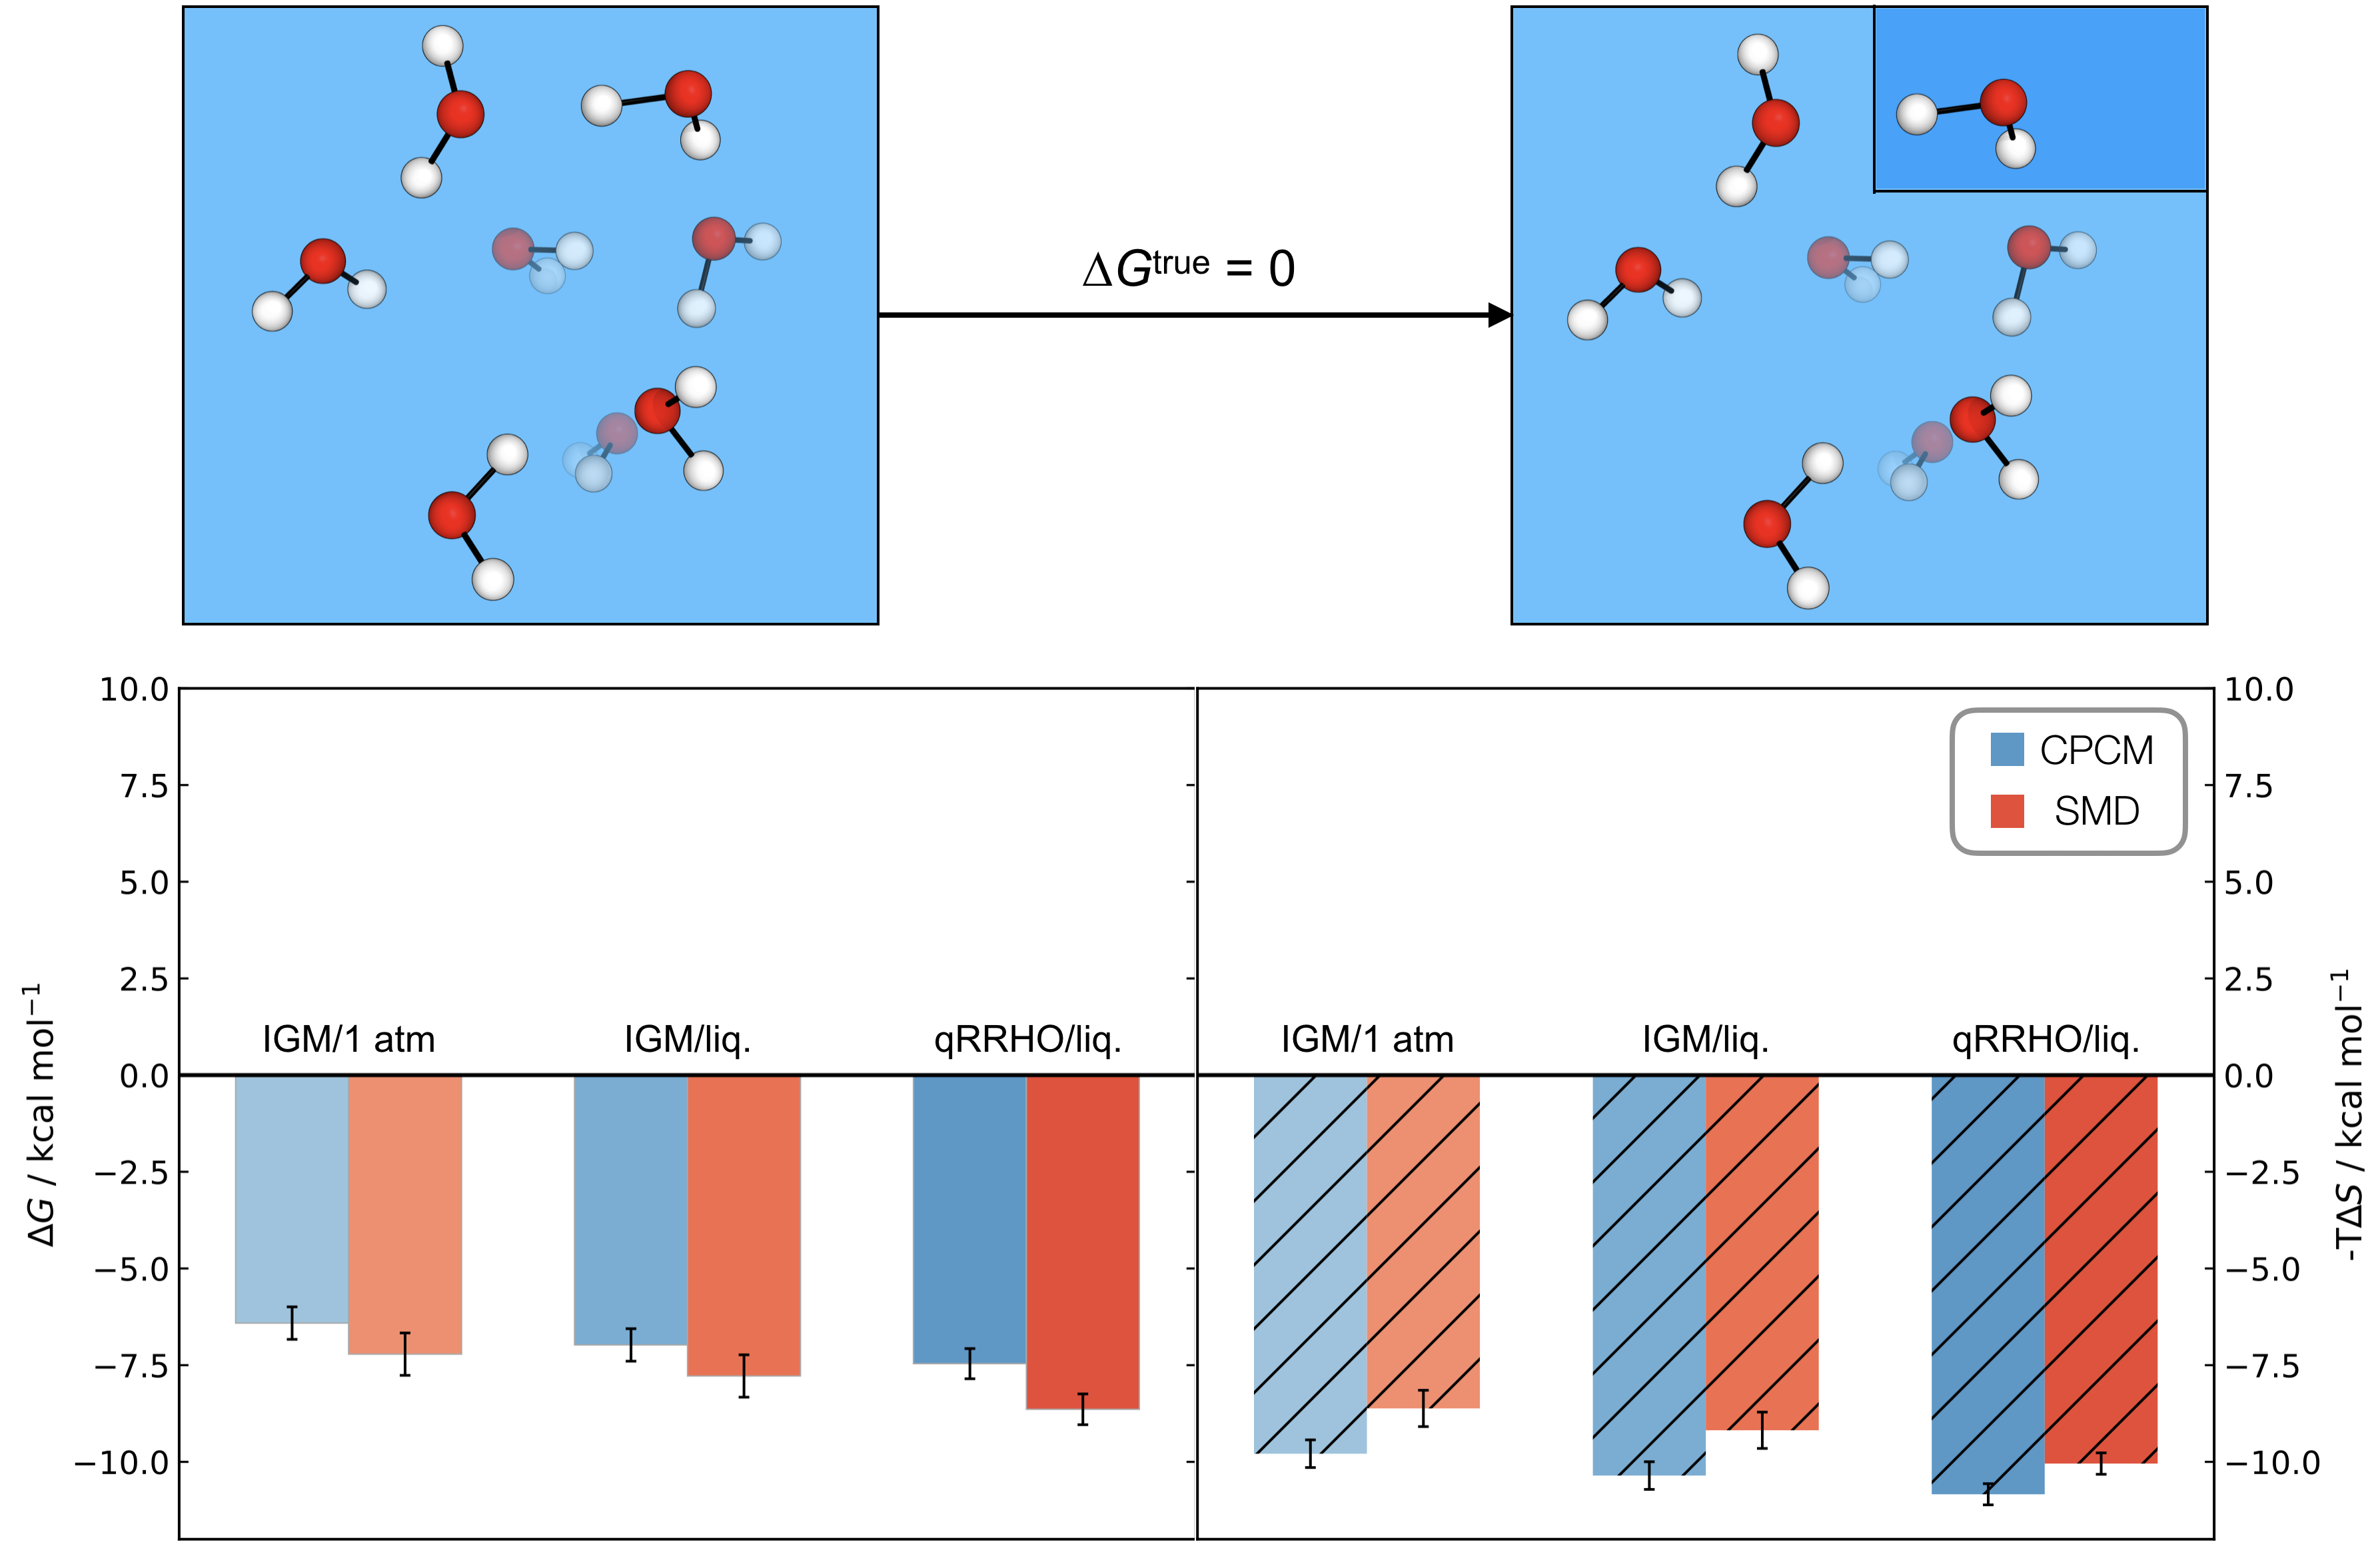
\includegraphics[width=\textwidth]{4/figs/figX2/figX2}
	\vspace{0.2cm}
	\hrule
	\caption{Free energy and entropy changes upon dissociation of a single water molecule from an octamer cluster immersed in implicit solvent modelled either with CPCM or SMD models (as implemented in ORCA). Potential energies calculated at DLPNO-CCSD(T)//def2-TZVPP//PBE0-D3BJ/def2-SVP and  error bars quoted as standard error of the mean over the possible dissociation events. States appropriate for a 1 atm pressure (default in electronic structure codes) and the appropriate $55.5/n$ M  molarity for a cluster of $n$ molecules in water (liq.) are shown. Snapshot taken randomly from a revPBE0-D3 quality classical simulation of 64 water molecules at 300 K.}
	\label{fig::entropy_X2}
\end{figure}

This is unsurprising when on the reactant side the translational entropy associated with a water molecule is treated as a vibration or rotation (within the qRRHO\cite{Grimme2012} approach) while on the right, the single water molecule has free translation within a PIB (and thus many more populated states). Likewise, with the rotational contribution, the motion on the left is approximated as harmonic (or between a HO and free rotor within qRRHO) and on the right a free rotor. Clearly, this distinction is unphysical and there should be no difference in treatment for each molecule on the left and right hand sides of the reaction.

\section{Translational Surface}
To use a more realistic treatment of the translational and rotational motion for a solute molecule in solution, the corresponding energy wells are required ($V_\text{trans}(x, y, z)$, $V_\text{rot}(R_x, R_y, R_z)$, where $R_k$ is a rotation around axis $k$). For a water-in-water system, the translational surface may be obtained by a time average over a simulation, which -- by analogy to the ergodic hypothesis -- should approach the average for many water molecules. Averaging the potential over frames from a revPBE0-D3 quality simulation of liquid water from ref. \cite{Young2021GAP} and displacing the most central water molecule in the Cartesian $x$-direction affords the section function $V_\text{trans.}(x, 0, 0)$ (\figurename{ \ref{fig::entropy_X3a}}). 

\begin{figure}[h!]
	\centering
	\begin{minipage}[b]{0.6\textwidth}
		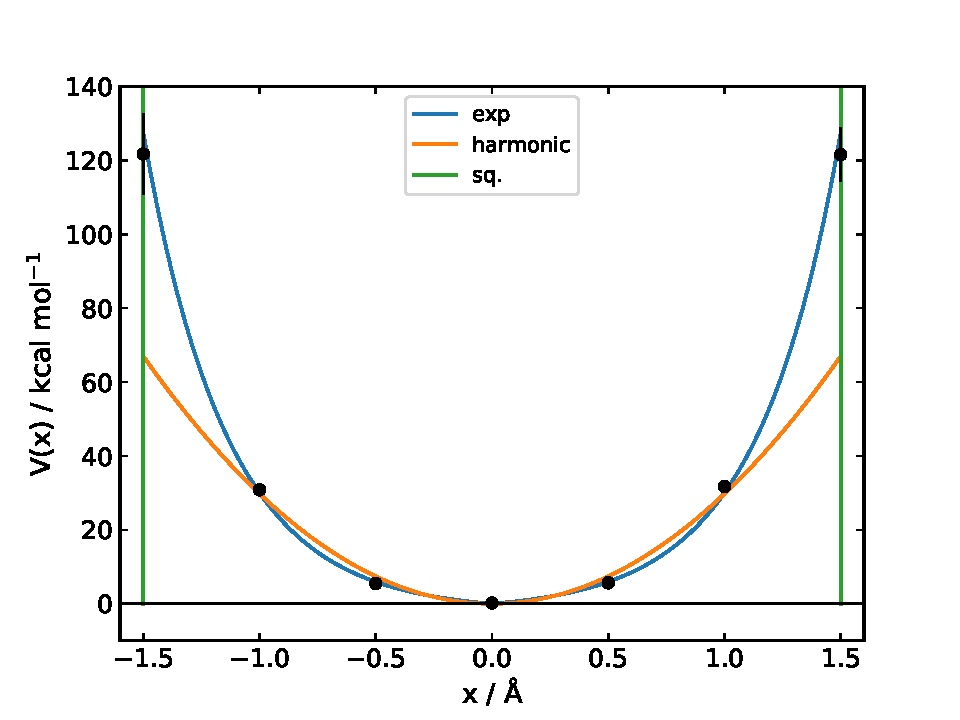
\includegraphics[width=9.5cm]{4/figs/figX3/dft_well.pdf}
	\end{minipage}
	\hfill
	\begin{minipage}[b]{0.39\textwidth}
		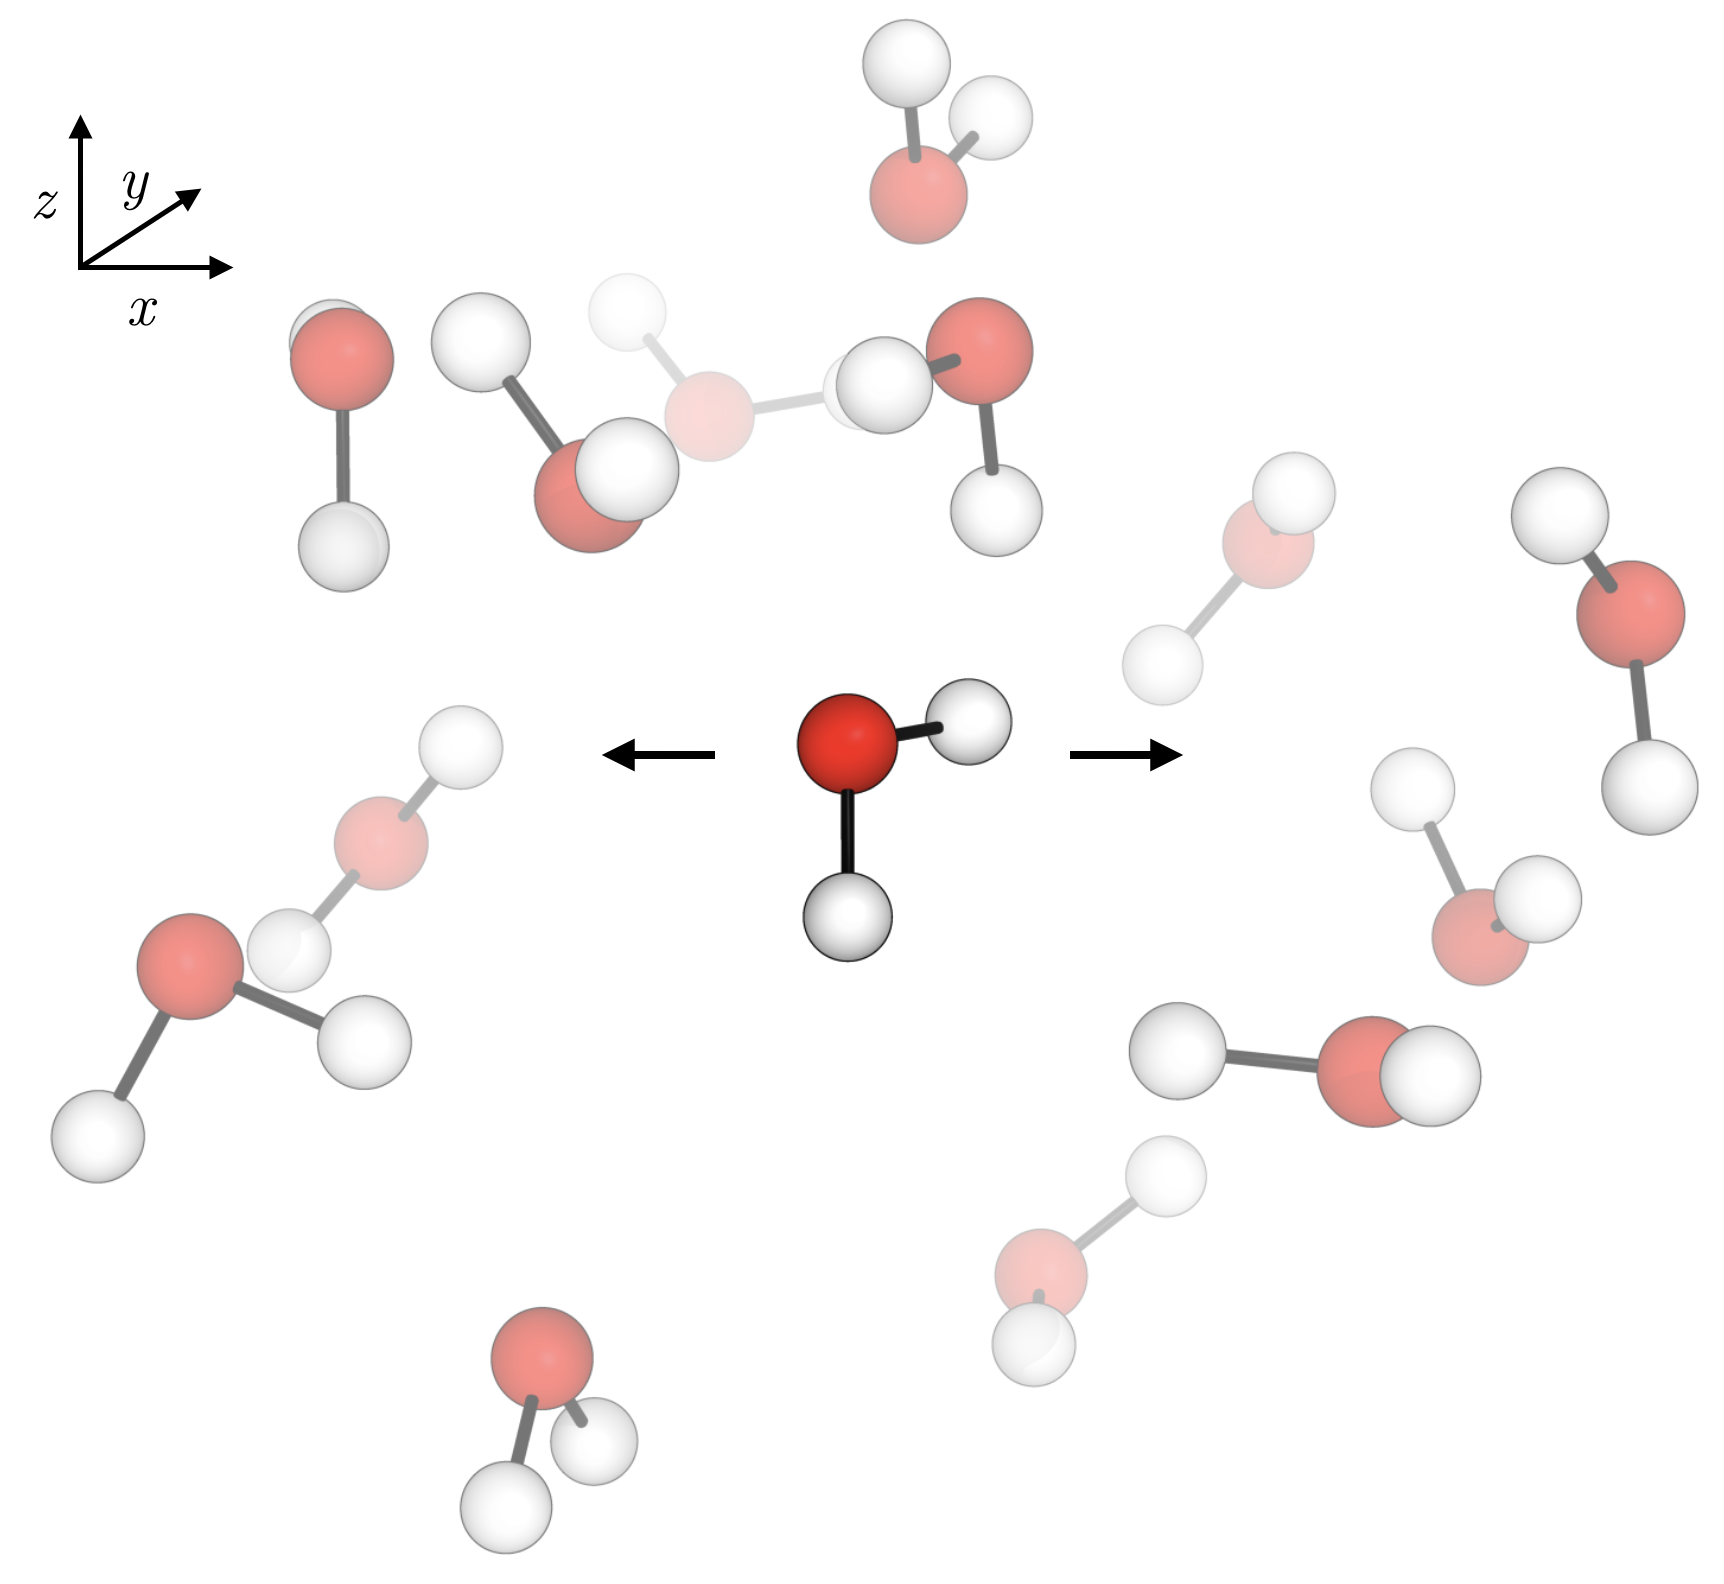
\includegraphics[width=6cm]{4/figs/figX3/dft_well_trns.png}
		\vspace{0.7cm}
	\end{minipage}
	\vspace{0.2cm}
	\hrule
	\caption{Translational potential energy surface for a water molecule in liquid water at 300 K (64 water molecules, cubic box, $l = 12.42$ \AA), black points. Surface averaged over 500 frames separated by 60 fs at the PBE0-D3BJ/def2-SVP level of theory. Clusters generated by including neighbouring water molecules within a 5 \AA$\;$ spherical distance, shifting in the Cartesian $x$-direction and evaluating the single point energy. A sample water cluster containing 14 water molecules within a 5 \AA$\;$ sphere is shown. Fitted functions (lines) correspond to exponential (exp, $V \sim e^{|x|}$), harmonic ($V \sim x^2$) and infinite square wells (sq. $V = 0 \text{ if }-1.5 < x < 1.5\text{, else } \infty$). Error bars shown as the standard error of the mean on all points.}
	\label{fig::entropy_X3a}
\end{figure}

Fitting these points to an infinite square well and harmonic potentials, with known QM eigenspectra, affords only moderate agreement to the averaged points on the potential.\footnote{Interestingly, Garza's method using the free-volume like approach to calculate the effective volume generates a similar estimate as the square well fit in \figurename{ \ref{fig::entropy_X3a}}. $V \approx v_c \; ; \; v_c = (V_\text{water}^{1/3} + V_\text{free}^{1/3})^3 \; ; \; V_\text{free} = M_\text{w} / N_A \rho - V_\text{water} \; ;\; V_\text{water} = 27.971$ \AA${}^3$ using a spherical approximation of water and radii from ref. \cite{CRC}
%import numpy as np
%import autode as ade
%from autode.atoms import get_vdw_radius
%h2o = ade.Molecule(smiles='O')
%coords = h2o.coordinates
%centroid = np.average(coords, axis=0)
%r_o = np.linalg.norm(coords[0] - centroid) + get_vdw_radius('O')
%r_h = np.linalg.norm(coords[0] - centroid) + get_vdw_radius('H')
%r = max(r_h, r_o)
%v_m = (4.0 * np.pi / 3.0) * r**3
%print(v_m)
%v_free = ((18.02 / 1000)         # M_w     in kg mol-1
%/
%(6.022E23             # N_a     in mol-1
%* 1000)              # density in kg m^3
%) * 1E30              # m^3 -> Å^3
%v_free -= v_m
%N_c = 1
%v_c = (v_m**(1/3) + v_free**(1/3))**3
%V = N_c * v_c
%print(V)
%print(f'l = {V**(1/3)}')	
, such that $v_c = 78.700$ \AA${}^3$ and the side length used in the PIB partition function $l = 4.285$ \AA.} In contrast, fitting an exponential well,
\begin{equation}
V_\text{trans}^\text{exp}(x) = k (e^{a|x|} - 1)
\end{equation}
where $k, a$ are parameters to be determined and $k$ has units of energy, affords an excellent agreement between the fit and the true values, which are within error on all points (\figurename{ \ref{fig::entropy_X3a}}). This agreement is not surprising considering short-range closed-shell (Pauli) repulsion has an exponential distance dependence.\cite{Bolliger2013} Indeed, in the empirical Buckingham potential %first used to model noble gases and now commonly used in molecular mechanics force fields, 
the pairwise repulsive term is exponential in distance.\cite{Buckingham1938} With a model for $V_\text{trans}$ in hand, the following sections explore faster methods to generate the averaged potential and its dependence on the solute and solvent.

\newpage
\subsection{Methodology Optimisation}
To limit the computational expense of the calculations used to generate the averaged translational potential\footnote{\figurename{ \ref{fig::entropy_X3a}} required 7 points $\times$ 500 frames = 3500 DFT single-point calculations.} the DFT calculations may be replaced by tight-binding DFT equivalents (\figurename{ \ref{fig::entropy_X3b}}). The well is identical to within the average standard error across the points arising from incomplete sampling: MAD = 2 \kcal \emph{ cf} avg. std. error = 3 \kcal.

\begin{figure}[h!]
	\centering
	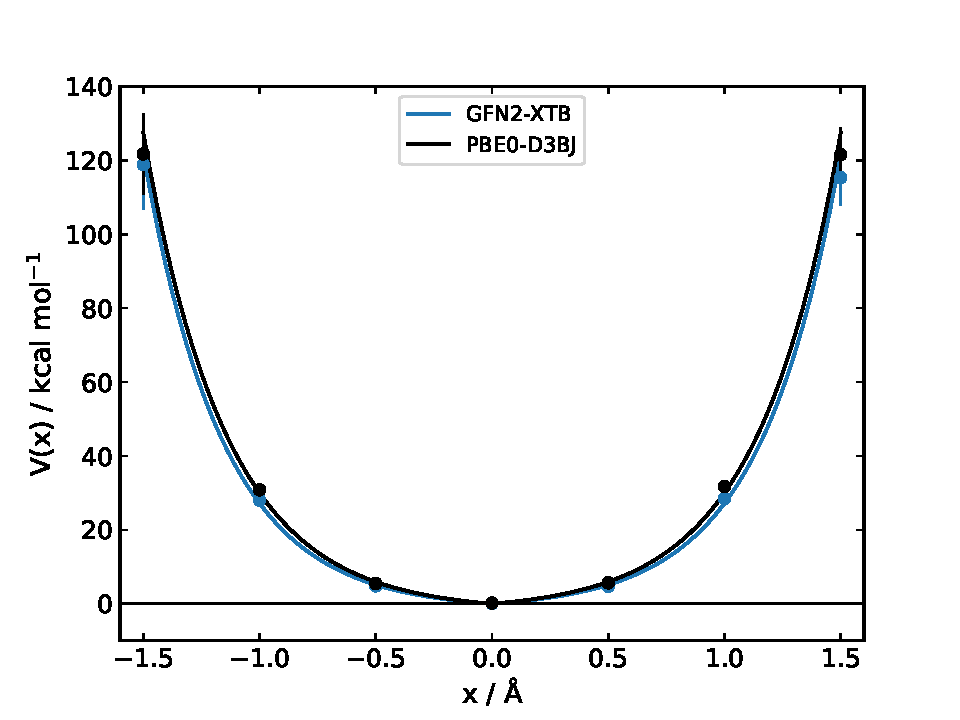
\includegraphics[width=10cm]{4/figs/figX3/dft_vs_xtb_well.pdf}
	\vspace{0.2cm}
	\hrule
	\caption{Comparison of GFN2-XTB and PBE0-D3BJ/def2-SVP surfaces for water-in-water. Trajectory frames taken as \figurename{ \ref{fig::entropy_X3a}}.}
	\label{fig::entropy_X3b}
\end{figure}

Likewise, while high quality AIMD simulations provide an accurate representation of the configuration space of the condensed phase system, they are computationally expensive. As such, it is be advantageous to employ a faster method to generate frames over which a potential is averaged. Comparing the translational surfaces of bulk liquid water from DFTB and molecular mechanics (TIP4P) MD frames there is a quantitative change to the exponential fits, but no qualitative difference (\tablename{ \ref{table::figX3c_params}}, \figurename{ \ref{fig::entropy_X3c}}).
\vspace{0.2cm}

\begin{figure}[h!]
	\centering
	\begin{minipage}[b]{0.49\textwidth}
		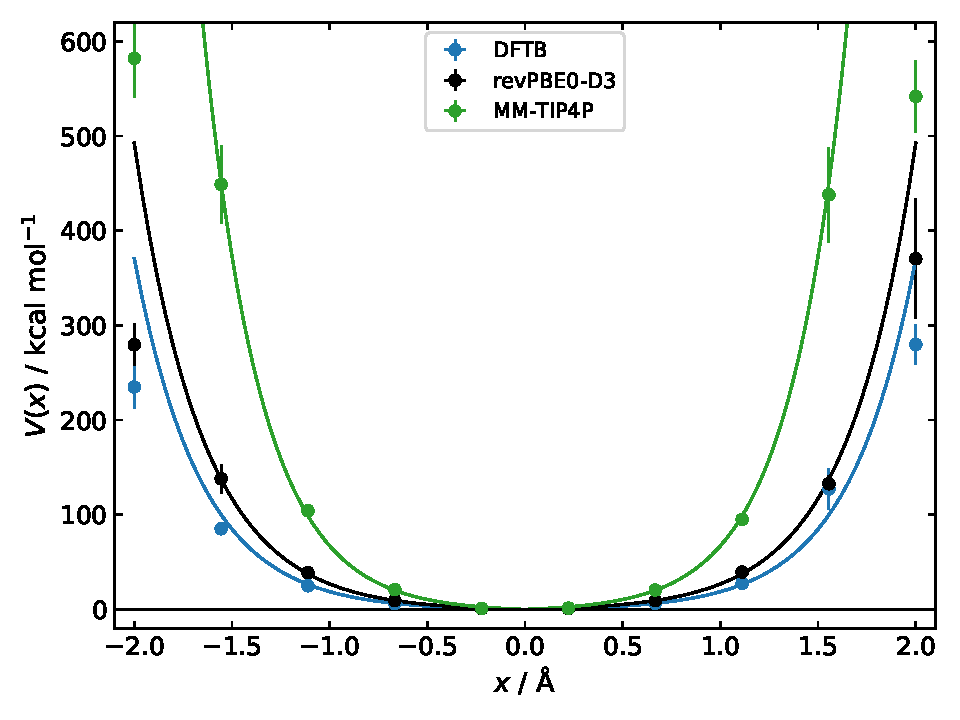
\includegraphics[width=8cm]{4/figs/figX3/xtb_wells.pdf}
	\end{minipage}
	\hfill
	\begin{minipage}[b]{0.49\textwidth}
		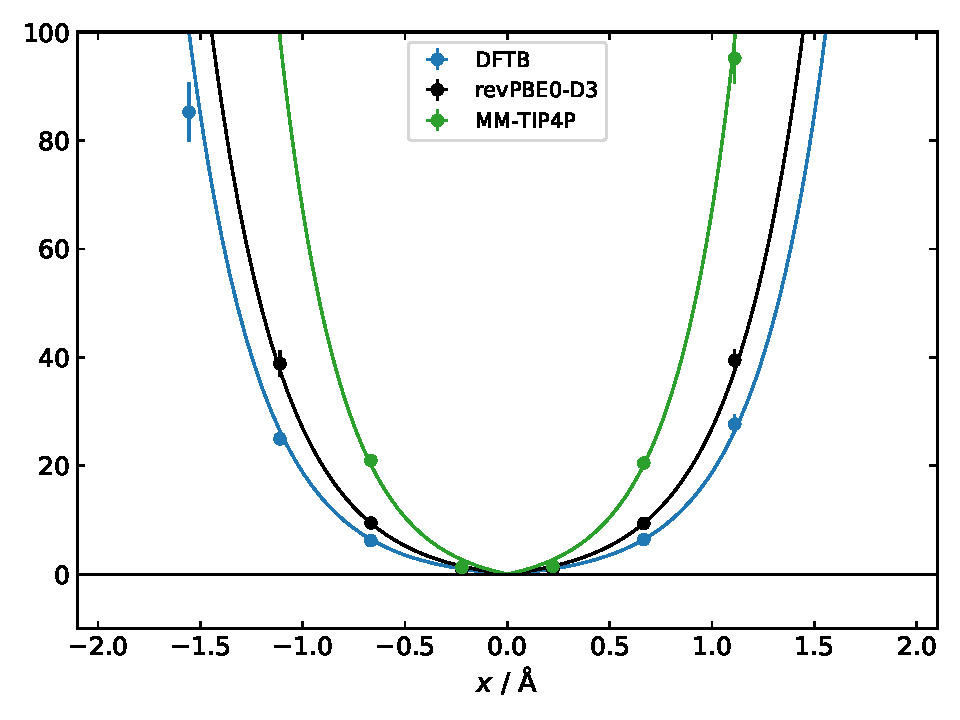
\includegraphics[width=8cm]{4/figs/figX3/xtb_wells_zoom.pdf}
	\end{minipage}
	\vspace{0.2cm}
	\hrule
	\caption{Comparison of methods to generate 500 frames over which the translational potential $V(x)$ is averaged for the water-in-water system. Frames generated from 300 K liquid water simulations of 30 ps using different reference methods to calculate energies and forces. DFTB used 3ob parameters while the molecular mechanics (MM) used TIP4P parameters, as implemented in GROMACS. Error bars are standard error of the mean.}
	\label{fig::entropy_X3c}
\end{figure}

% DFTB	k = 1.057 kcal mol-1	a = 2.931 Å-1
% revPBE0-D3	k = 1.65 kcal mol-1	a = 2.851 Å-1
% MM-TIP4P	k = 2.377 kcal mol-1	a = 3.375 Å-1

\begin{table}[h!]
	\renewcommand{\arraystretch}{1.5}
	\begin{center}
		\small
		\begin{tabularx}{\textwidth}{YYY} 
			\toprule
			Method & $k$ / \kcal & $a$ / \AA$^{-1}$ \\
			\hline
			DFTB             &   1.057  & 2.931 \\
			revPBE0-D3  &   1.650  & 2.851 \\
			MM-TIP4P     &   2.377 & 3.375 \\
			\bottomrule
		\end{tabularx}
	\end{center}
	\caption{Fitted parameters for exponential wells shown in \figurename{ \ref{fig::entropy_X3c}}.} 
	\label{table::figX3c_params}
\end{table}

Compared to the reference DFT-quality simulation, DFTB and MM under/overestimate the confinement of a water molecule within the solvent cage respectively, with the latter deviating more significantly. Given molecular tumbling and solvent reorganisation is a reasonably fast process,\footnote{From the Stokes-Einstein relation for the rotational diffusion coefficient $\tau \sim 4\beta\eta r^3$, where $r$ is the molecular radius and $\eta$ the viscosity, which yields $\tau \sim O(10^{-12})$ for small molecules.} short time dynamics should be sufficient to sample all the relevant configurations for small molecules. Therefore, DFTB simulations provide a good compromise between accuracy and computational cost, where reference simulations are not available. With associated errors on $k$ being $\sim 50$ \% and on $a \sim 2$ \% from only the methodology choice, any predictions must include that error.


\subsection{2D and 3D Surfaces}

To ensure the exponential well is a good approximation beyond the $V_\text{trans}(x, 0, 0)$ section function and generalises to the other Cartesian directions, the corresponding 2D and 3D surfaces were generated for CO$_2$ in water. Fitting 2D exponential and harmonic wells to the averaged surface shows the former is a much better approximation to the true potential (\figurename{ \ref{fig::2d_co2_in_h2o_mm_xtb}}). This is also obtained over a wider energy window than shown for the water-in-water system, cementing its applicability. The corresponding 3D potential is more challenging to compare, requiring a fourth dimension in energy, but does convey the spherical symmetry. The equivalence of $V_\text{trans}$ in all directions is unsurprising, as the potential is evaluated in the `lab' frame and thus the choice of direction is arbitrary when averaged over solute and solvent rotations. Given its spherical symmetry, it is then puzzling why the translational partition function is most commonly evaluated from an infinite cubic well, when the eigenspecturm for the analogous spherical well is known.\cite{Huang2016}

\begin{figure}[h!]
	\vspace{0.2cm}
	\centering
	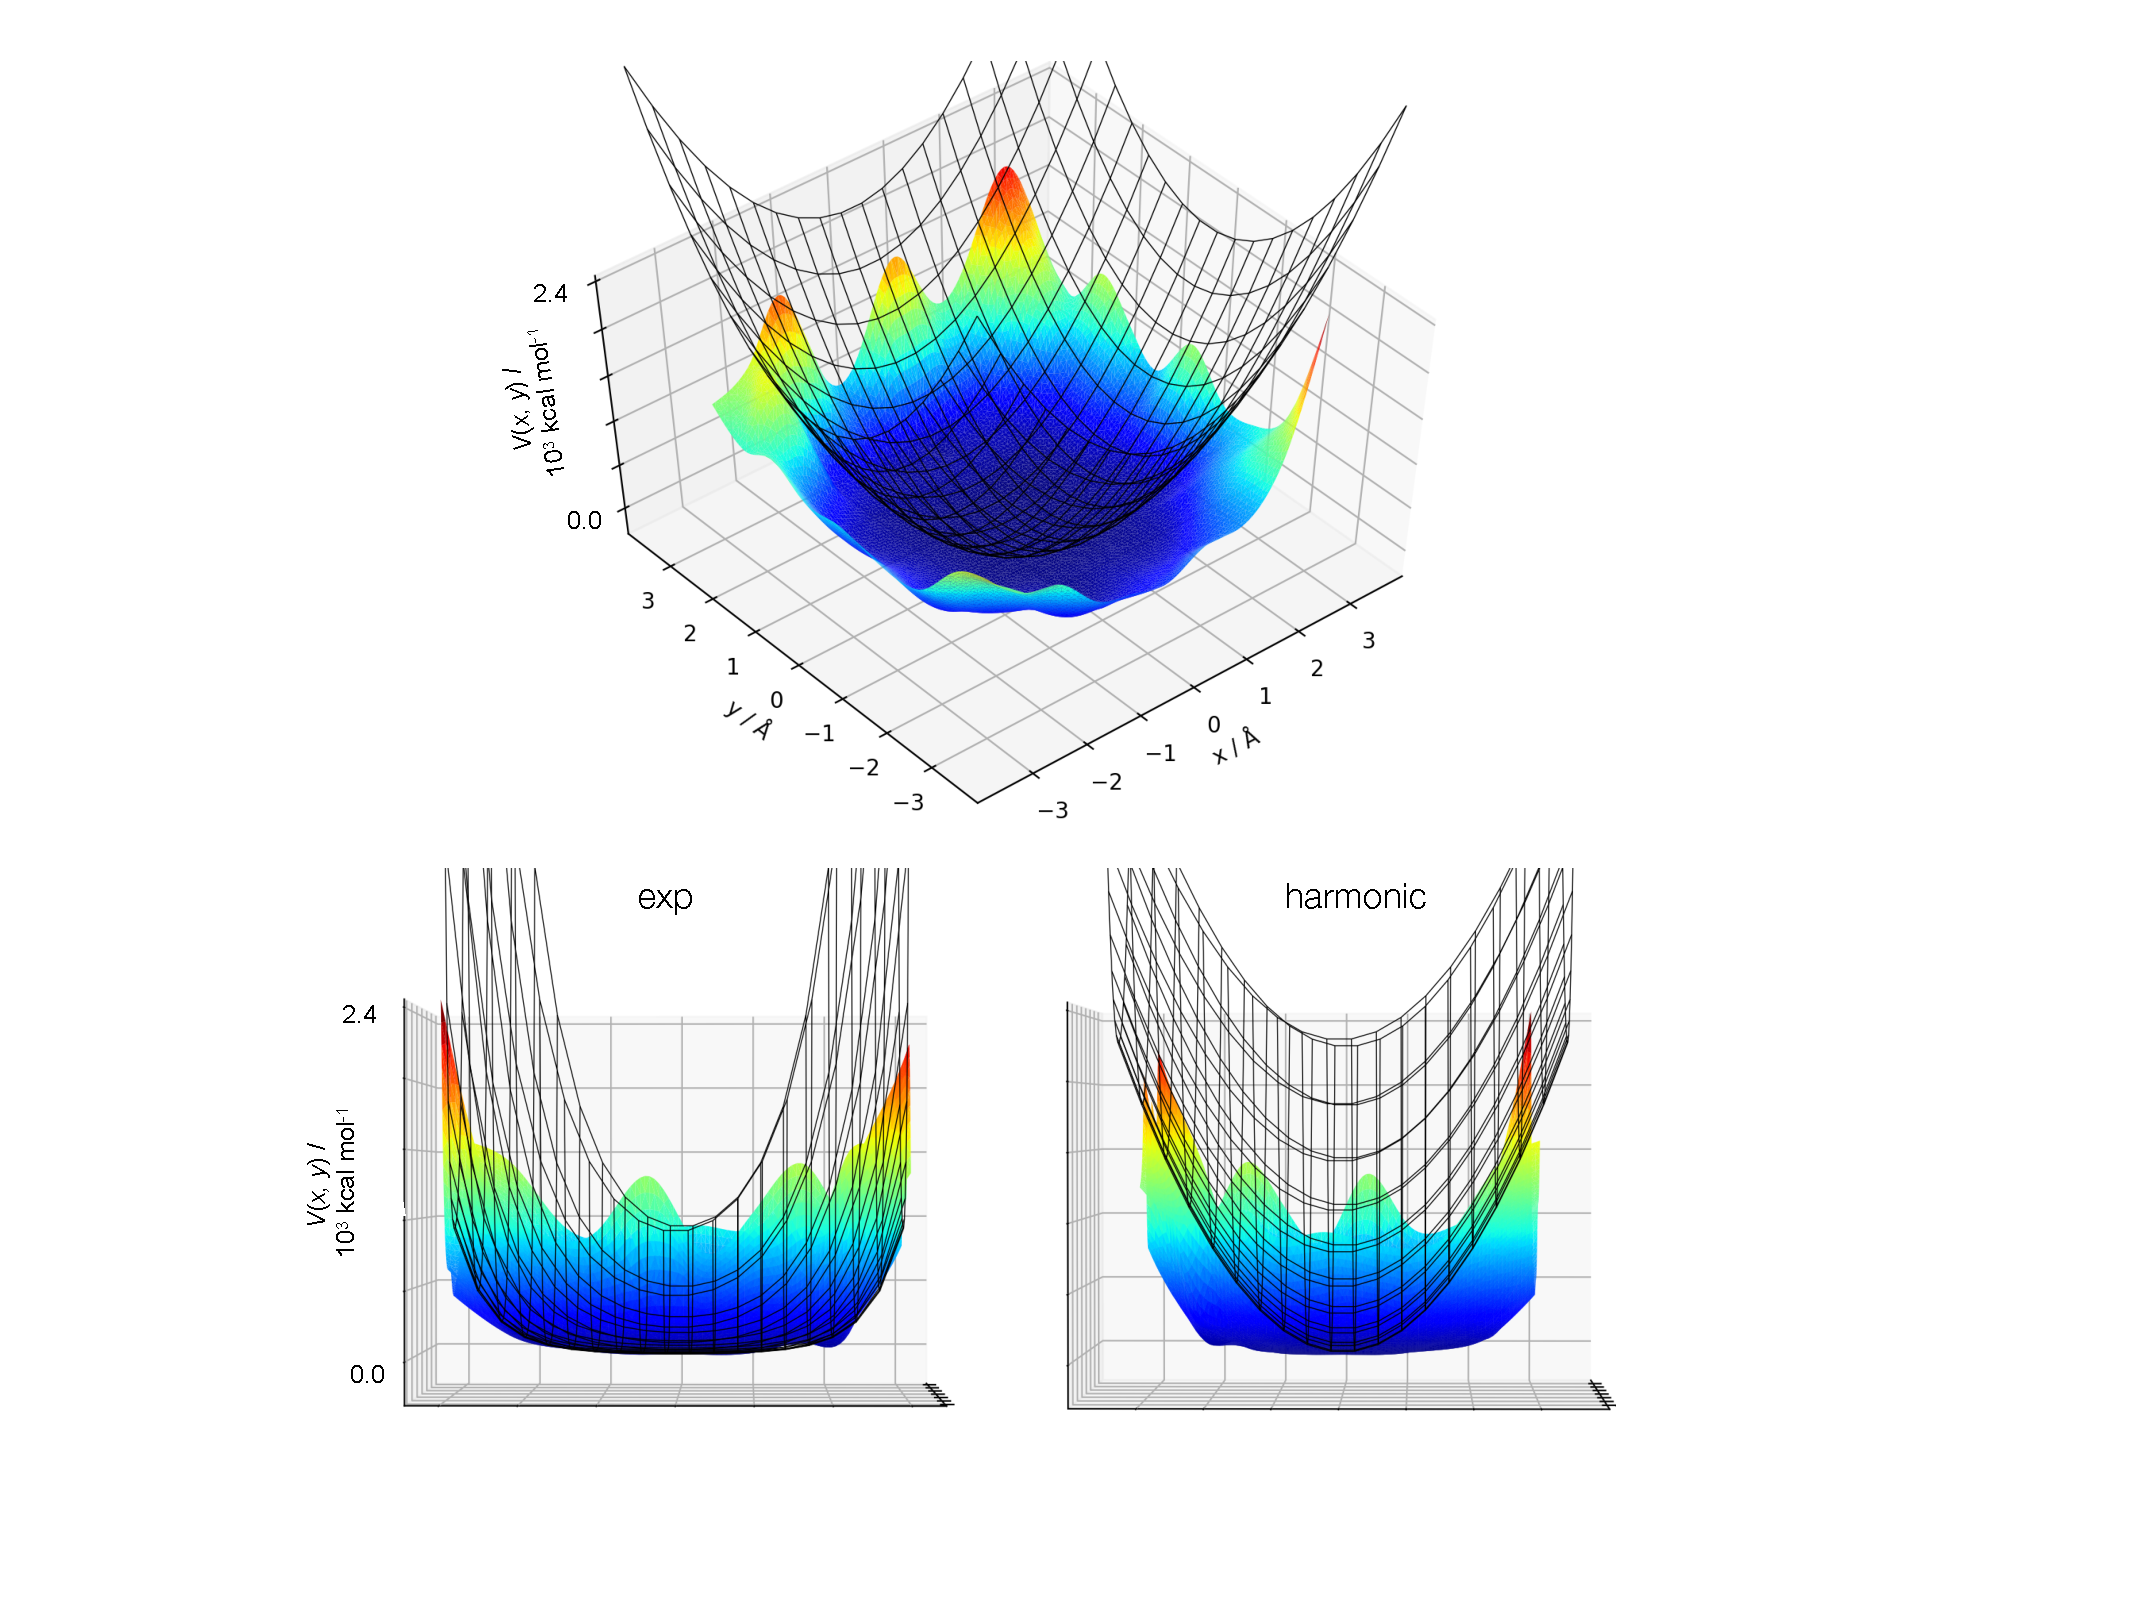
\includegraphics[width=14cm]{4/figs/figX4/figX4.pdf}
	\vspace{0.2cm}
	\hrule
	\caption{Translational potential energy surface for CO$_2$ in water evaluated by averaging GFN2-XTB single point energies over 100 frames separated by 1 ps obtained at the GAFF-TIP4P MM level using a 300 K $NVT$ simulation.} 
	\label{fig::2d_co2_in_h2o_mm_xtb}
\end{figure}


% ----------------------------------------  spherical..... ----------------------
\iffalse
\begin{figure}[h!]
	\vspace{0.2cm}
	\centering
	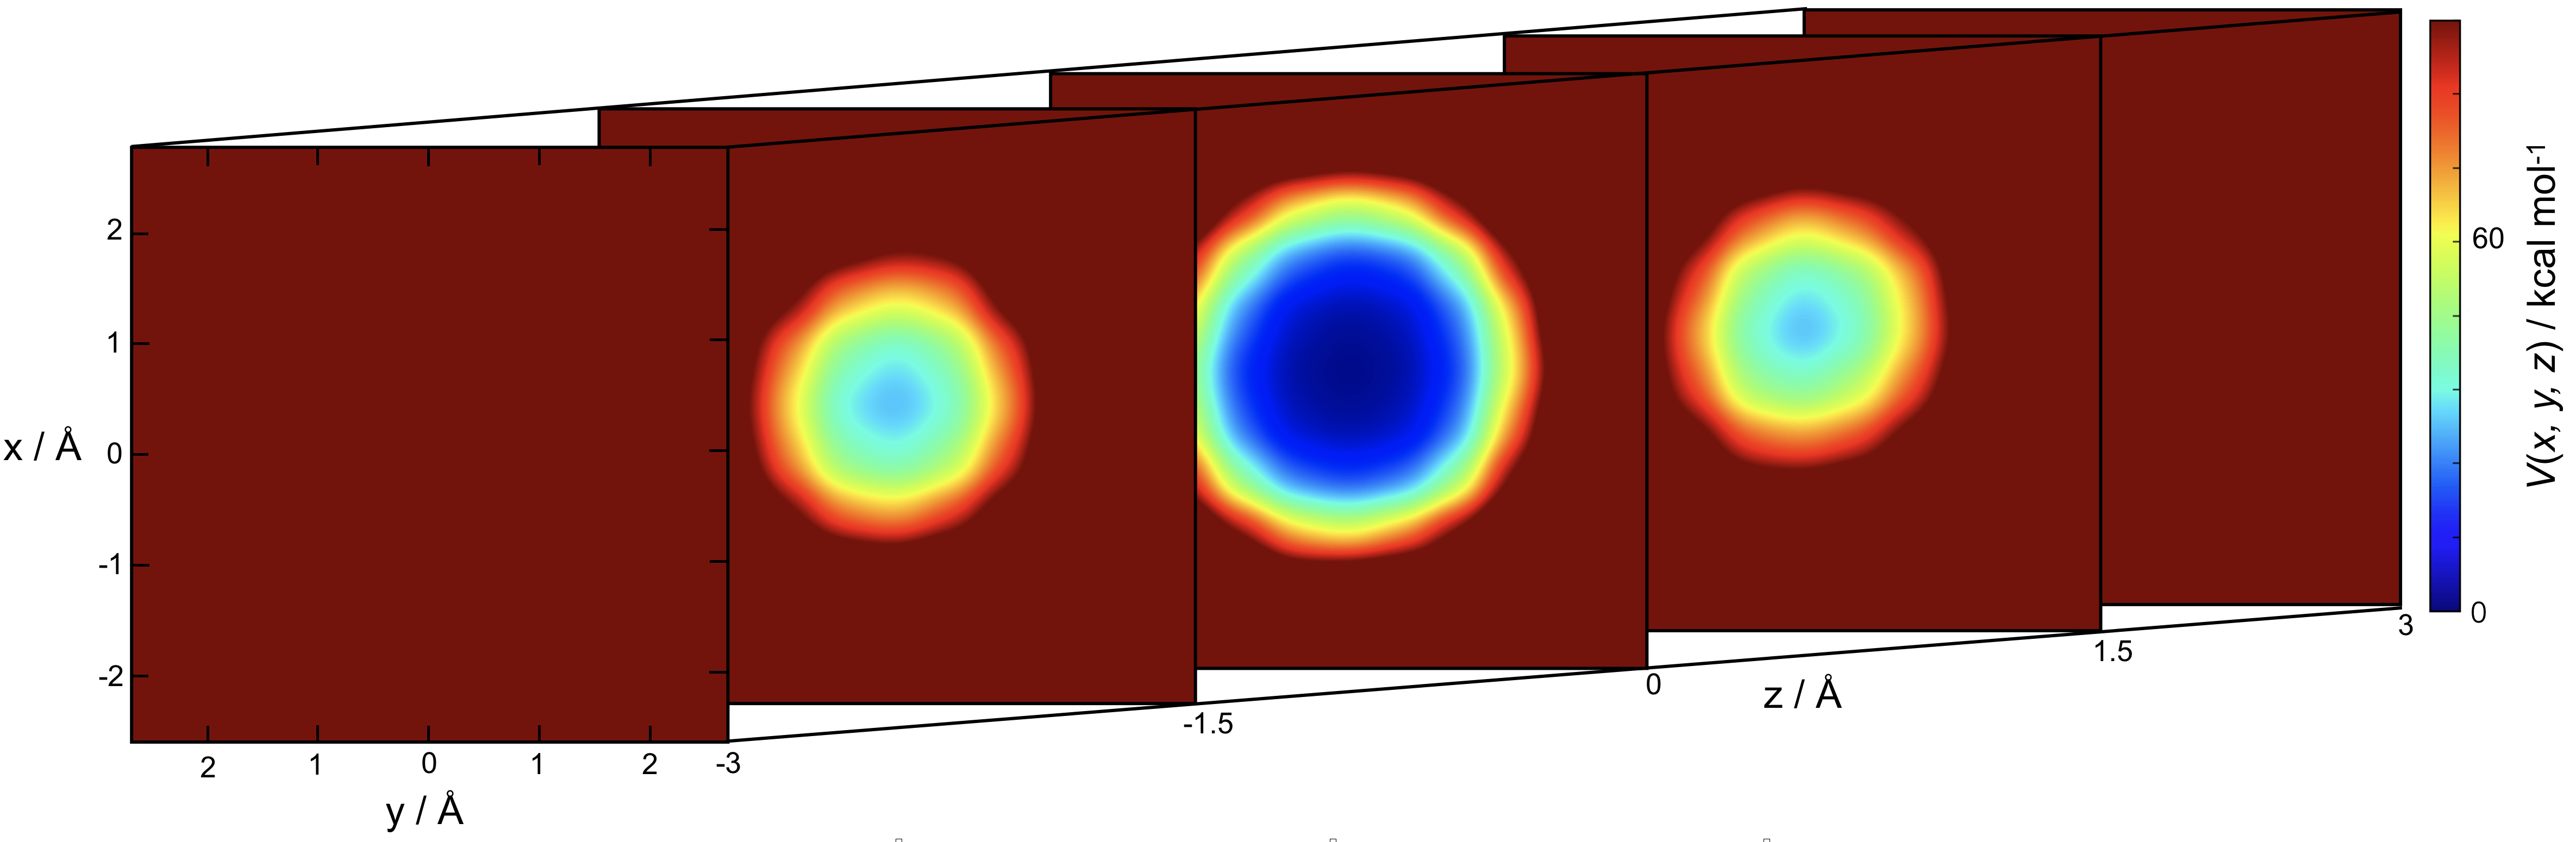
\includegraphics[width=\textwidth]{4/figs/figX4/3d_co2_in_h2o_mm_xtb}
	\vspace{0.2cm}
	\hrule
	\caption{As \figurename{ \ref{fig::2d_co2_in_h2o_mm_xtb}} in 3D averaged over 1000 points.} 
	\label{fig::3d_co2_in_h2o_mm_xtb}
\end{figure}
\fi
% --------------------------------------------------------------------------



\subsection{Solute and Solvent Dependence}

To develop a  widely applicable model that does not rely on explicitly solvated dynamics to generate parameters the solute and solvent dependence of the potential is required. To sample a range of interaction types in the solvation of  molecules CO$_2$, methane and alanine in water, acetonitrile and benzene were selected. In all cases an exponential well is an excellent approximation to the translational potential (\figurename{ \ref{fig::entropy_X5}}). 

Correlating $k$ and $a$ for the solute-solvent systems reveals they are reasonably independent and, although some broad trends can be extracted, generating a model for \emph{a priori} prediction of $k$ and $a$ may be challenging. Immediately, from \tablename{ \ref{table::figX5_params}} both parameters are tightly clustered ($k \sim 1$ \kcal and $a \sim 2.6 $ \AA$^{-1}$) irrespective of the system. Furthermore, solvents with a higher number density, such as water are  closer to the solute and thus generate a more enclosed cavity with a larger $a$. Unfortunately, this is not uniformly observed; CO$_2$ in benzene has amongst the largest $a$, which precludes a predictive model to avoid the time-consuming simulations. Nevertheless, with appropriate error bars on the derived quantities a semi-quantitative prediction may be made based on average parameters ($\bar{k}, \bar{a}$). 

\vspace{0.2cm}
\begin{figure}[p!]
	\centering
	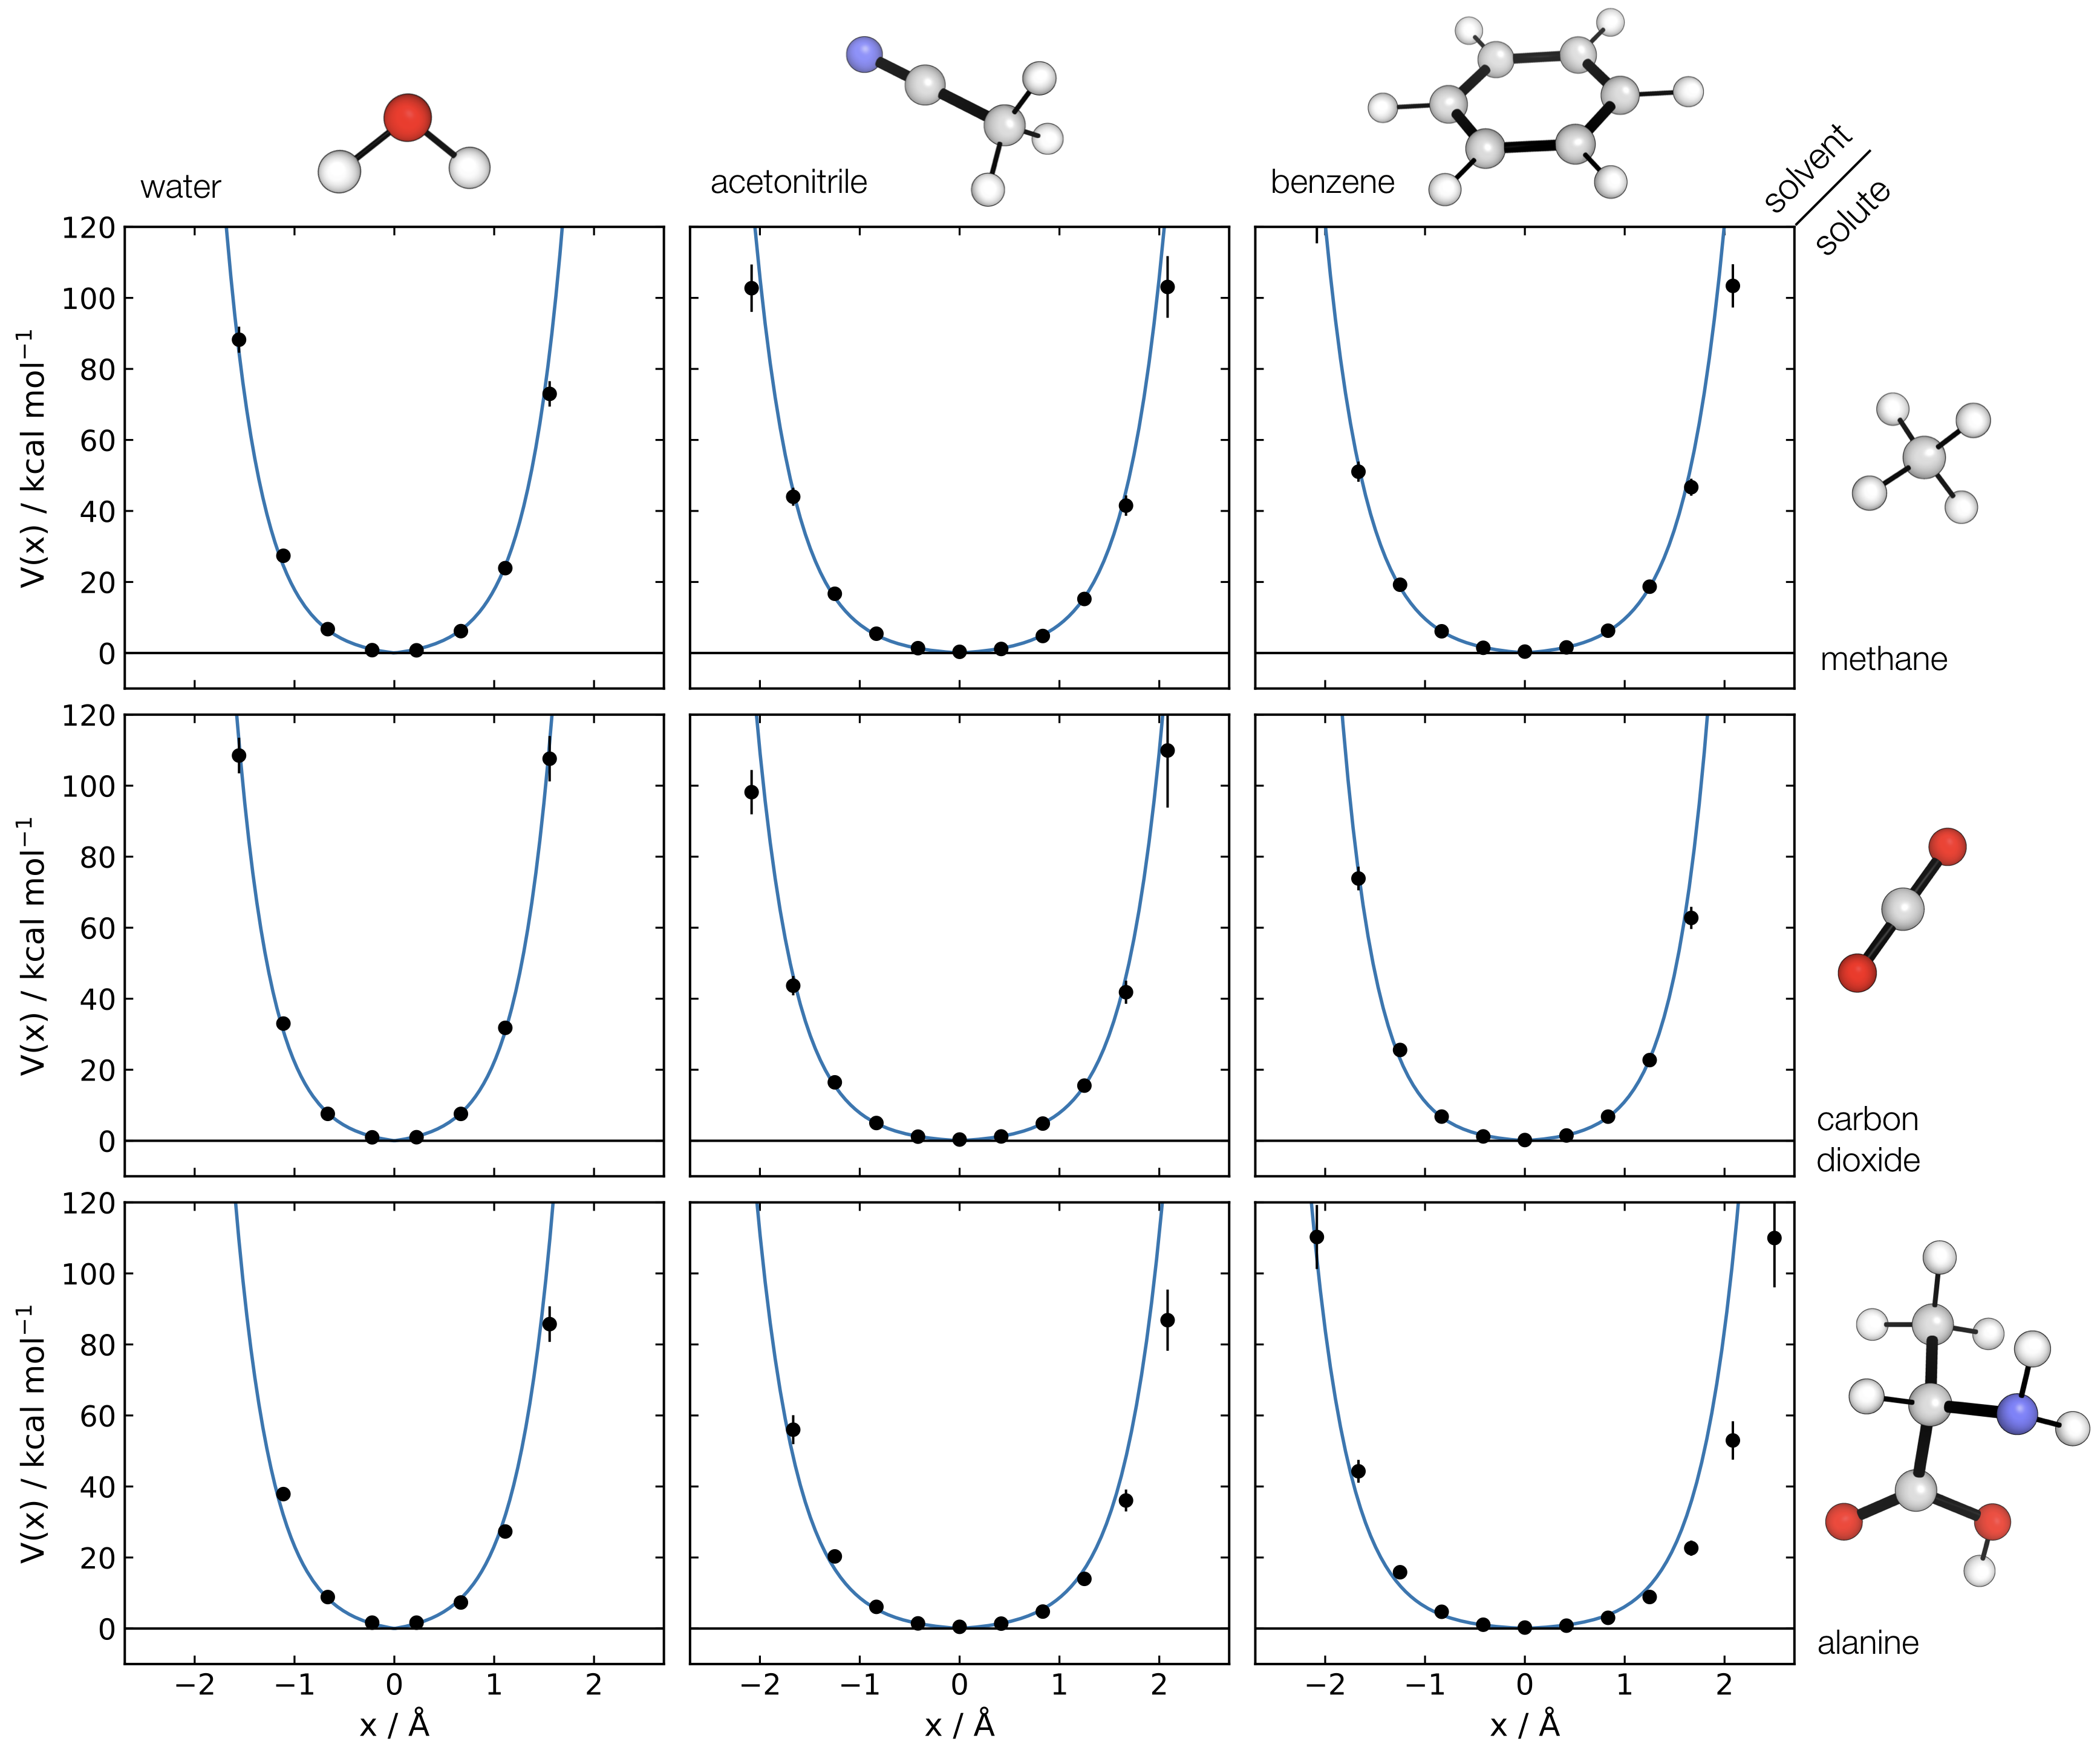
\includegraphics[width=\textwidth]{4/figs/figX5/figX5.png}
	\vspace{0.2cm}
	\hrule
	\caption{Translational potential energy surfaces for the displacement of solute molecules immersed in an explicit solvent. Points are averaged over 500 evenly spaced frames selected from 20 ps DFTB(3ob) 300 K Langevin dynamics in a cubic box ($l = 12$ \AA) with a number of solvent molecule to reach the solvent density, excluding the solute volume. Potentials calculated using displacements of $\approx 0.35$ \AA$\,$ displacements in the $x$-direction. Error bars plotted as the statistical error of the mean over frames. Fully solvated clusters extracted from the periodic simulations by taking solvent molecules within 5 \AA$\;$ sphere around the solute. Overlaid exponential wells fit as \figurename{ \ref{fig::entropy_X3a}}.}
	\label{fig::entropy_X5}
\end{figure}

%methane-in-water k = 1.278 kcal mol-1 a = 2.705 Å-1
%methane-in-mecn k = 0.718 kcal mol-1 a = 2.5 Å-1
%methane-in-benzene k = 0.911 kcal mol-1 a = 2.449 Å-1
%co2-in-water k = 1.386 kcal mol-1 a = 2.832 Å-1
%co2-in-mecn k = 0.655 kcal mol-1 a = 2.562 Å-1
%co2-in-benzene k = 0.707 kcal mol-1 a = 2.809 Å-1
%alanine-in-water k = 1.692 kcal mol-1 a = 2.688 Å-1
%alanine-in-mecn k = 0.796 kcal mol-1 a = 2.473 Å-1
%alanine-in-benzene k = 0.524 kcal mol-1 a = 2.542 Å-1

\begin{table}[h!]
	\renewcommand{\arraystretch}{1.5}
	\begin{center}
		\small
		\begin{tabularx}{\textwidth}{YYYY} 
			\toprule
			Solute & Solvent& $k$ / \kcal & $a$ / \AA$^{-1}$ \\
			\hline
			Methane  & Water &   1.278    &   2.705     \\
			Methane  & Acetonitrile &   0.718    &   2.500    \\
			Methane  & Benzene &   0.911    &    2.449    \\
			CO$_2$  & Water&   1.386    &    2.832     \\
			CO$_2$  & Acetonitrile&   0.655    &    2.562   \\
			CO$_2$  & Benzene &    0.707   &    2.809   \\
			Alanine   &Water &     1.692  &    2.688     \\
			Alanine   & Acetonitrile&   0.796    &    2.473   \\
			Alanine   & Benzene &   0.524   &   2.542    \\
			\hline
			Average && 1.0 ± 0.4 & 2.6 ± 0.1 \\
			\bottomrule
		\end{tabularx}
	\end{center}
	\caption{Fitted parameters for exponential wells shown in \figurename{ \ref{fig::entropy_X5}} at the GFN2-XTB//DFTB(3ob) level of theory.} 
	\label{table::figX5_params}
\end{table}

\newpage
\section{Translational Entropy from Spherical Wells}
Given the average potential for solute translation is spherical, and well approximated by an exponential well (EW), the partition function must be obtained in order to calculate the translational entropy more accurately than the IGM approximation. 

\subsection{Infinite Spherical Well}

First, considering the limiting infinite (step function) case of the exponential well, for an infinite spherical well the potential is given by,

\begin{equation}
V(\boldsymbol{r}) = 
\begin{cases}
0 \qquad\;\; \text{if} \quad 0 \le |\boldsymbol{r}| < c \\
\infty \qquad \text{if} \quad  c \ge |\boldsymbol{r}| \\
\end{cases}
\end{equation}
the Schrodinger equation is soluble,\cite{Huang2016} and the eigenvalues are given by,
\begin{equation}
E_{l.n} = z_{l, n}^2 \frac{\hbar^2}{2mc^2}
\end{equation}
where $z_{l, n}$ is the $n$'th zero of the $l$'th spherical Bessel function, and $E_{l.n}$ is $2l+1$ fold degenerate. For a light particle (1 amu) in a small cavity (radius, $c = 2$ au) the partition function converges rapidly with $n, l$ which are evaluated on a rectangular grid converged in both $n$ and $l$. The classical partition function for this potential is,

% ------------------------------------------- Non essential methods ---------------------------

% (\figurename{ \ref{spherical_well_eigenvalue_sum_2au_1882amu}}a). 

\iffalse
The roots are found by evaluating the spherical Bessel function $j_l(x)$ between 0 and $\max(x)$, with spacing $\delta x$. The error in $Z$ decreases dramatically with step size (\figurename{ \ref{spherical_well_eigenvalue_sum_2au_1882amu}}b).

\begin{figure*}[h!]
	\begin{subfigure}[t]{0.5\textwidth}
		\centering
		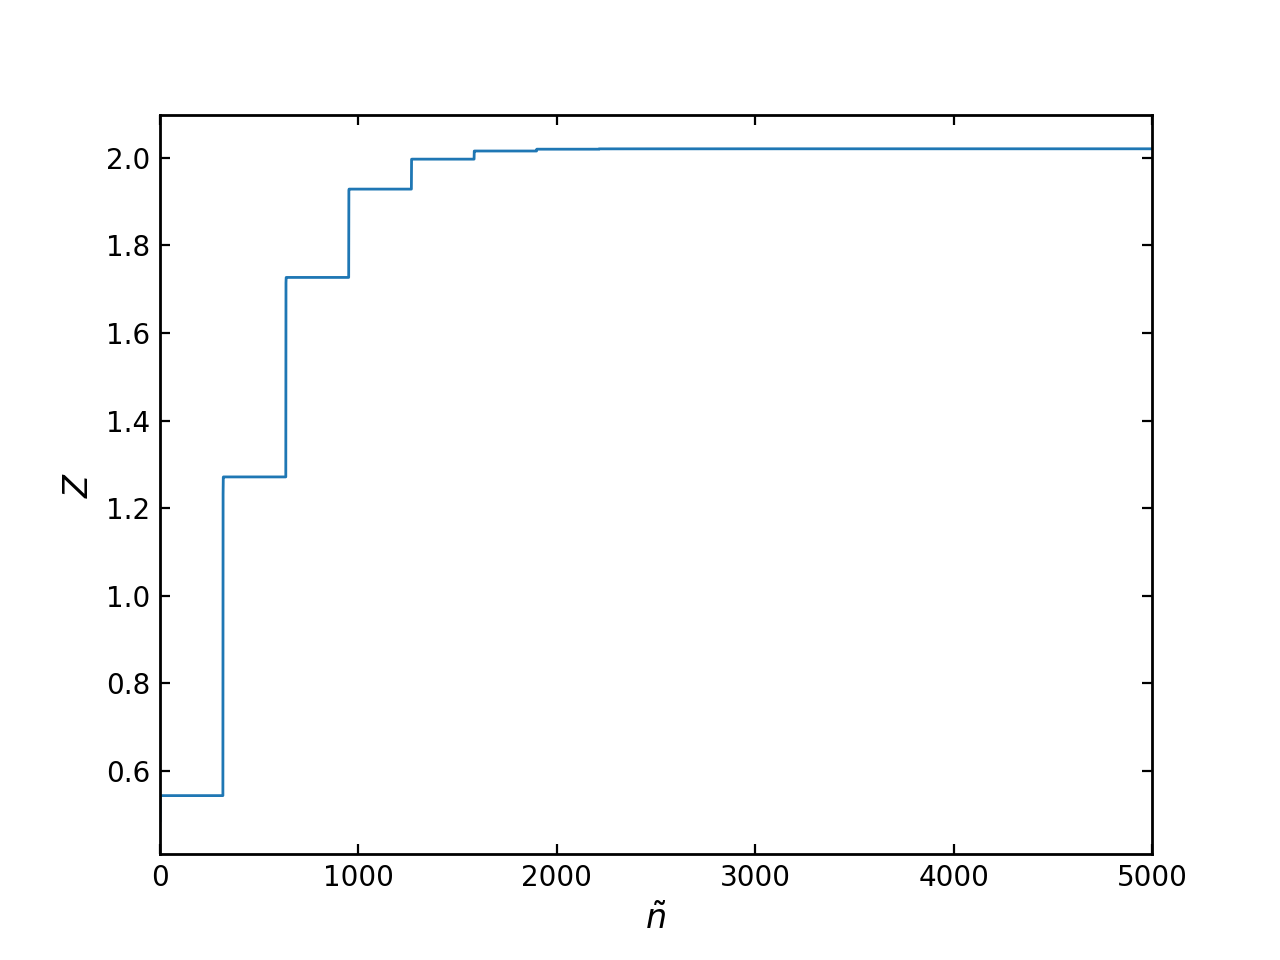
\includegraphics[height=6.2cm]{4/figs/spherical_well_eigenvalue_sum_z_vs_tilde_n}
		\caption{}
	\end{subfigure}%
	~ 
	\begin{subfigure}[t]{0.5\textwidth}
		\centering
		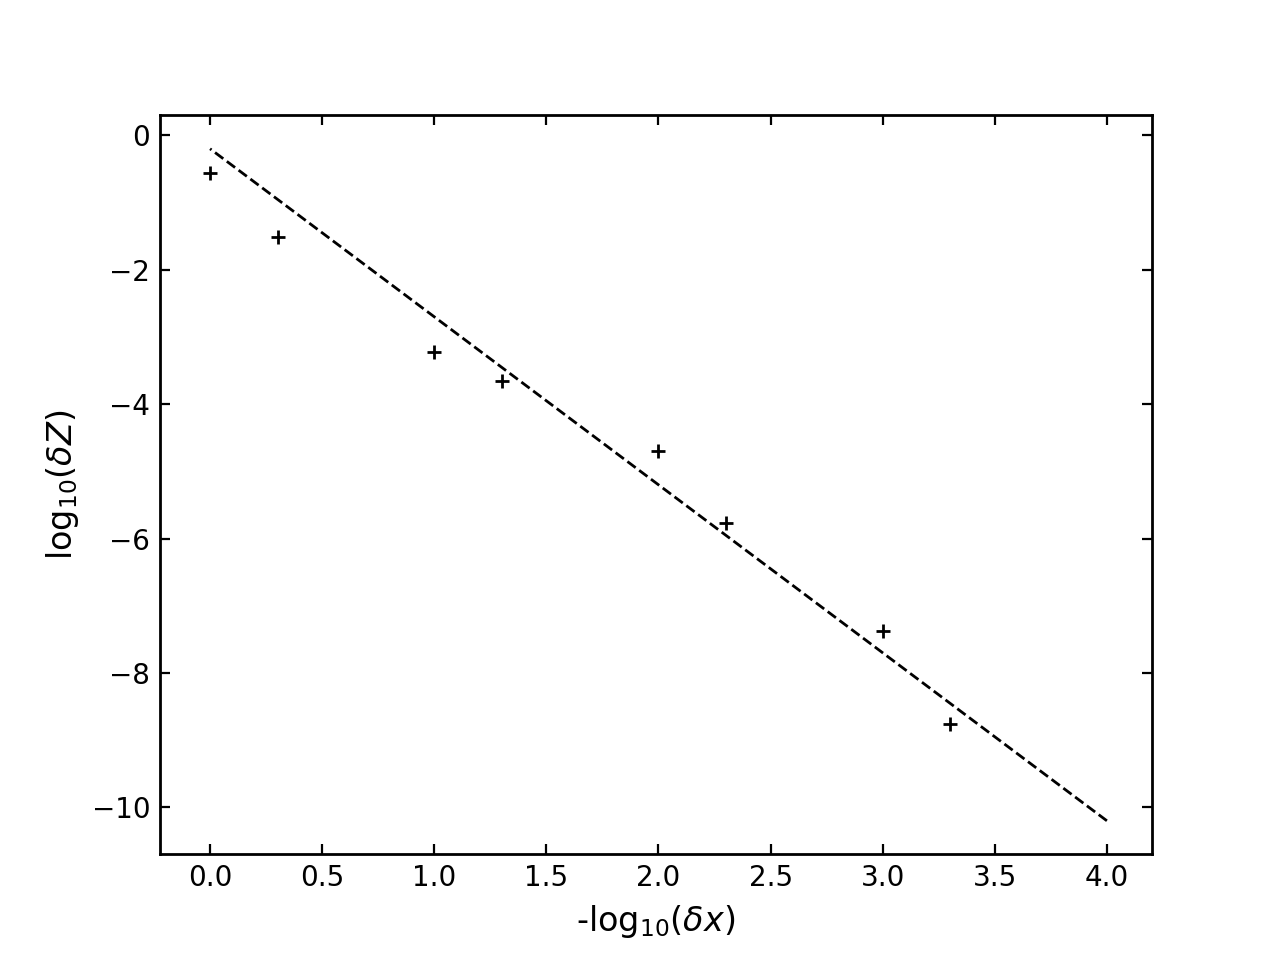
\includegraphics[height=6.2cm]{4/figs/spherical_well_eigenvalue_sum_delta_x_vs_delta_z}
		\caption{}
	\end{subfigure}
	\vspace{0.2cm}
	\hrule
	\caption{(a) Quantum partition function $Z$ vs the number of eigenvalues included in the summation $\tilde{n}$ ($\delta x = 10^{-2}$). (b) Error in $Z$ ($\delta Z$) vs the separation of $x$ values for root finding ($\delta x$). $c = 2.0 \text{ au.}, m = 1 \text{ amu}, \max(x) = 10^3, \max(l) = 10^2$. Roots of $j_l(x)$ are found over the range $x \in [0, \max(x)]$.} 
	\label{spherical_well_eigenvalue_sum_2au_1882amu}
\end{figure*}
\fi
% ---------------------------------------------------------------------------------

\begin{equation}
\begin{aligned}
Z_c &= \frac{1}{h^{3}}\int\int e^{-\beta H(\boldsymbol{p}, \boldsymbol{x})} \; d\boldsymbol{p}^{3} d\boldsymbol{x}^{3} \\
&= \frac{1}{h^{3}}\int_{-\infty}^\infty e^{-\beta \boldsymbol{p}^2/2m} \; d\boldsymbol{p}^{3} \int_{-\infty}^\infty e^{-\beta V(x, y, z)} \;  d\boldsymbol{x}^{3} \\
&= {\Big (} \frac{2\pi m k_B T}{h^2} {\Big )}^{3/2}  \int_0^c e^{-\beta \cdot 0}  4\pi r^2\;  dr \\
%&= {\Big (} \frac{2\pi m k_B T}{h^2} {\Big )}^{3/2}  4\pi \int_0^c r^2\;  dr \\
&= {\Big (} \frac{2\pi m k_B T}{h^2} {\Big )}^{3/2} \frac{4\pi c^3}{3} \\
\end{aligned}
\end{equation}
and the classical entropy,
\begin{equation}
\begin{aligned}
S_c &= k_B T \frac{1}{Z_c} \frac{\partial Z_c}{\partial T} + k_B \ln(Z_c) \\
&= k_B T {\Big (} \frac{h^2}{2\pi m k_B T} {\Big )}^{3/2} \frac{3}{4\pi c^3} {\Big (} \frac{2\pi m k_B}{h^2} {\Big )}^{3/2} \frac{4\pi c^3}{3}\cdot \frac{3}{2}T^{1/2} + k_B \ln(Z_c) \\
&= \frac{3k_B}{2} + k_B \ln(Z_c)
\end{aligned}
\end{equation}

The quantum and classical PFs for two systems are calculated as a function of the number of eigenvalues ($\bar{n}$) included in the summation (\figurename{ \ref{spherical_well_quantum_classical}}). These are a reasonably classical system, with eigenvalues separated by far less than $k_BT$ ($c = 20$ au, $m = 48$ amu) and a more quantum one of a H$_2$ molecule in a cavity with radius 1 \AA (\figurename{ \ref{spherical_well_quantum_classical}}).

\begin{figure*}[b!]
	\begin{subfigure}[t]{0.49\textwidth}
		\centering
		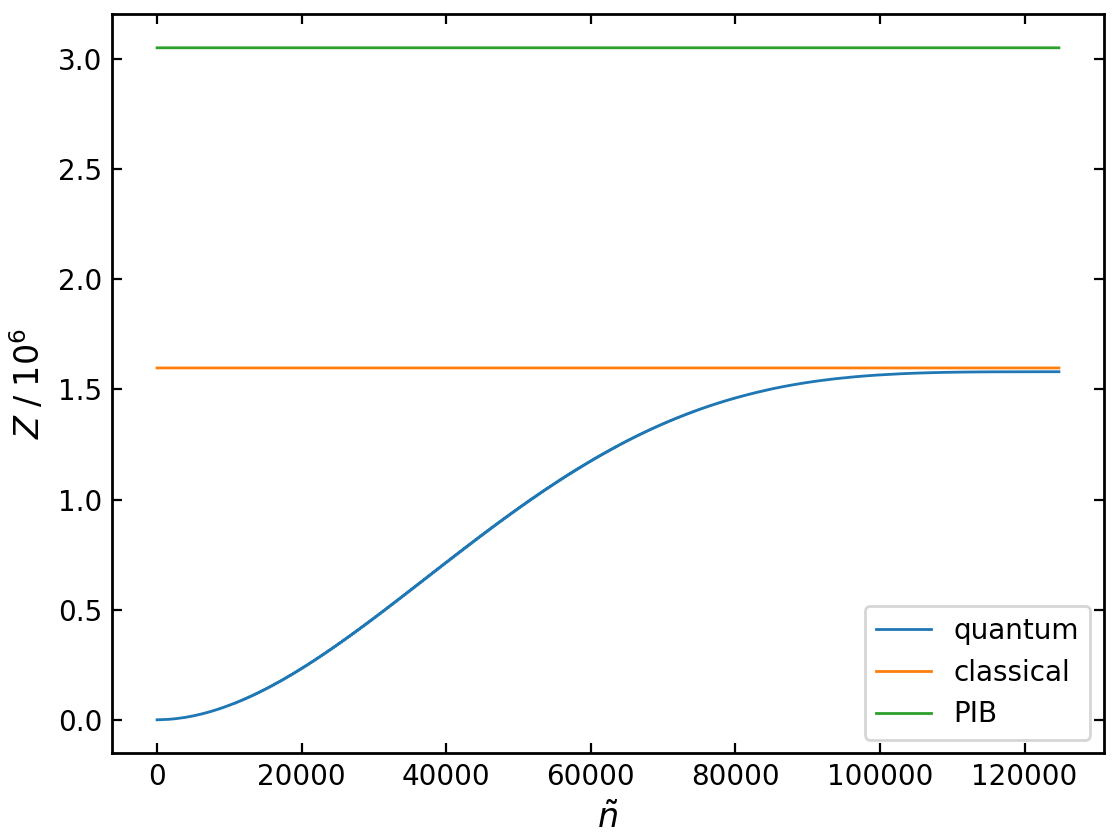
\includegraphics[height=6.2cm]{4/figs/spherical_well_20_c_87456_m_point1_dx_pf}
		\caption{}
	\end{subfigure}%
	~ 
	\begin{subfigure}[t]{0.49\textwidth}
		\centering
		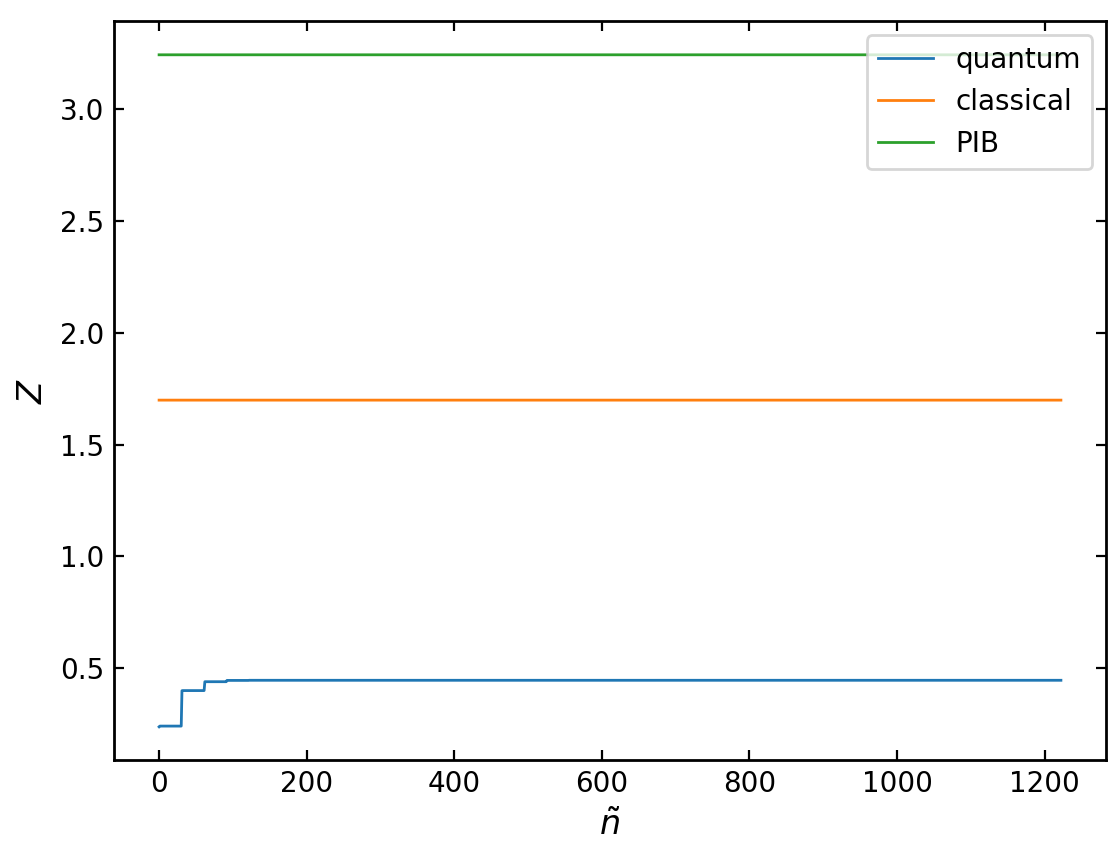
\includegraphics[height=6.2cm]{4/figs/spherical_well_1_c_3644_m_pf}
		\caption{}
	\end{subfigure}
	\vspace{0.2cm}
	\hrule
	\caption{$Z$ for a particle in a sphere (a) $c = 20$ au, $m = 48$ amu, $\delta x = 10^{-1},\;\max(x) = 10^3,\;\max(l) = 10^3$ and (b) $c = 1$ au, $m = 2$ amu, $\delta x = 10^{-2} ,\;\max(x) = 10^2,\;\max(l) = 10^2$. The partition function for a PIB (using the integral approximation) with $l = 2c$ is also plotted.} 
	\label{spherical_well_quantum_classical}
\end{figure*}


As expected for the classical system $Z$ converges to its classical analogue (\figurename{ \ref{spherical_well_quantum_classical}}a). The PF for H$_2$ translation is, however, not well reproduced classically with an overestimation of a factor of 3 compared to the quantum analogue (\figurename{ \ref{spherical_well_quantum_classical}}b). However, in the vast majority of cases the classical PF is likely to be a sufficient approximation, particularly as the entropy depends on the log of the PF.

For a system of mass 48 amu and $c = 2$ \AA the PFs converge to within 5\% and the resultant entropy to within 0.2 J K$^{-1}$ mol$^{-1}$ at $\tilde{n} = 10^5$, well below the acceptable error (\figurename{ \ref{spherical_well_z_s_qunat_classical}}). Interestingly, a particle in a cubic box treatment with a side length equal to the diameter of the sphere is a reasonable approximation to the spherical analogue, with only a $\sim 5$ J K mol$^{-1}$ difference in the corresponding entropy.

\begin{figure*}[h!]
	\centering
	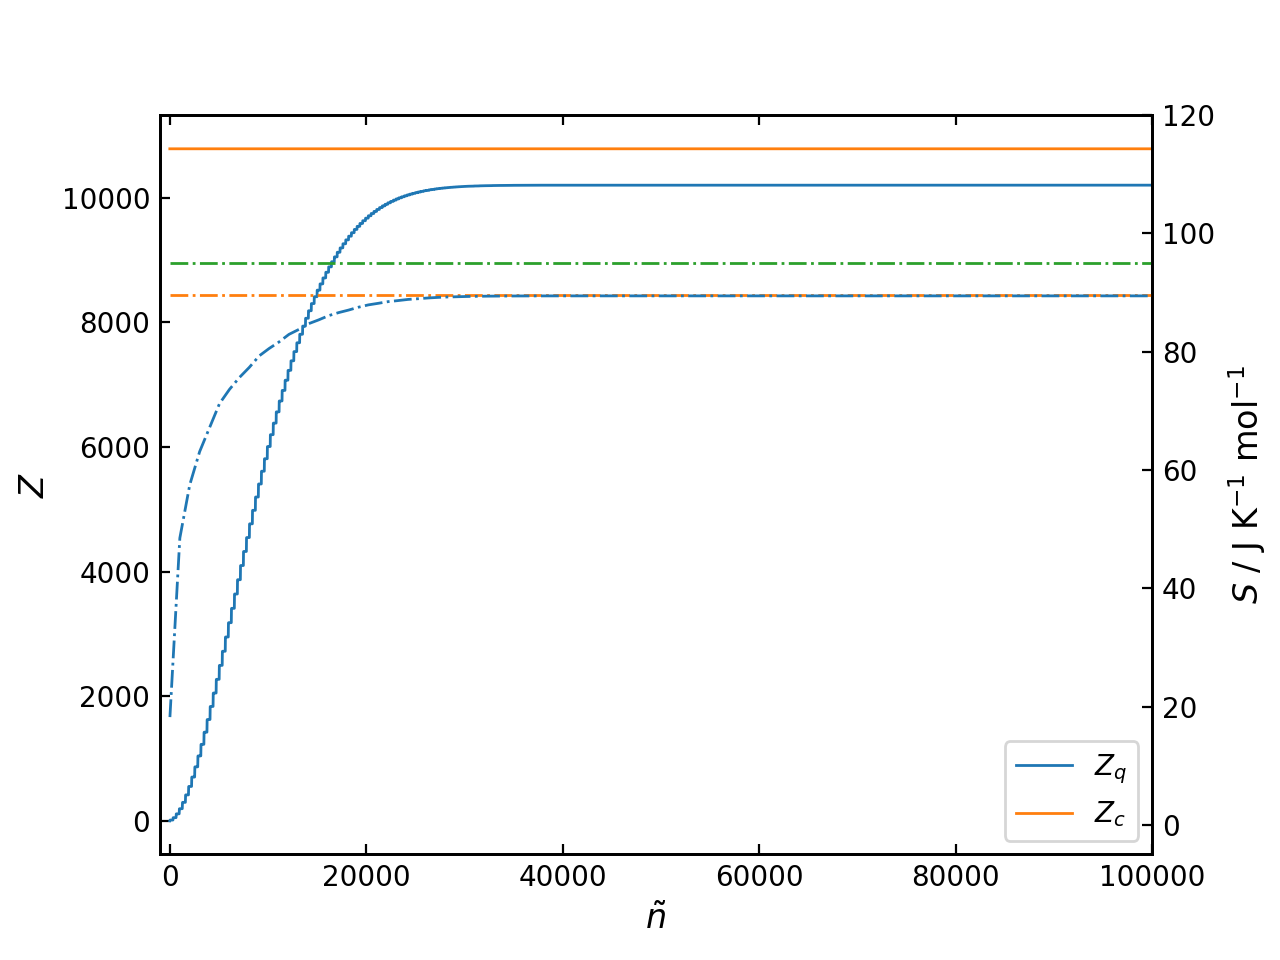
\includegraphics[height=7.5cm]{4/figs/spherical_well_z_s_qunat_classical}
	\vspace{0.2cm}
	\hrule
	\caption{Classical and quantum PFs (solid lines) and entropy (dot-dashed lines) vs the number of eigenvalues included in the summation ($\bar{n}$). PIB entropy (green) and classical (orange) and quantum (blue) particle in a sphere. $m =$ 48 amu and $c = 2$ \AA, $T$ = 298.15 K. $\partial Z / \partial T$ evaluated numerically $\delta T = 10^{-8}$ K.} 
	\label{spherical_well_z_s_qunat_classical}
\end{figure*}


\subsection{Exponential Well}
For a spherical potential of the form $V(\boldsymbol{r}) = k e^{a|\boldsymbol{r}|}$ no exact analytic solution of the time-independent Schroedinger equation exists. As such, the eigenvalues must be either approximated or found numerically. For simplicity, the 1D case ($V(x) = k e^{a|x|}$) is considered initially, the eigenstates of which are solutions of,
\begin{equation}
\begin{aligned}
\hat{H}\Psi(x) &= E \Psi(x) \\
{\Big \{} -\frac{1}{2m} \frac{d^2}{d x^2} + k e^{a|x|} {\Big \}}\Psi(x) &= E\Psi(x) \\ 
\Psi''(x) + 2m(k e^{a|x|} - E)\Psi(x) &= 0 \qquad : x \in \mathbb{R}
\end{aligned}
\label{1d_exp_well_SE}
\end{equation}
with boundary conditions $\Psi(-\infty) =  \Psi(\infty) = 0$ ensuring the WF is normalisable. Seemingly this potential also does not have an analytic solution.\footnote{An exponential potential on $x \in [0, \infty)$ with $\Psi(0)=\Psi(\infty)=0$ has been solved.\cite{Amore2008}} As such, the eigenstates and associated eigenfunctions are found numerically (\figurename{ \ref{wf_1d_exp_well_numerical}}).

\begin{figure*}[h!]
	\centering
	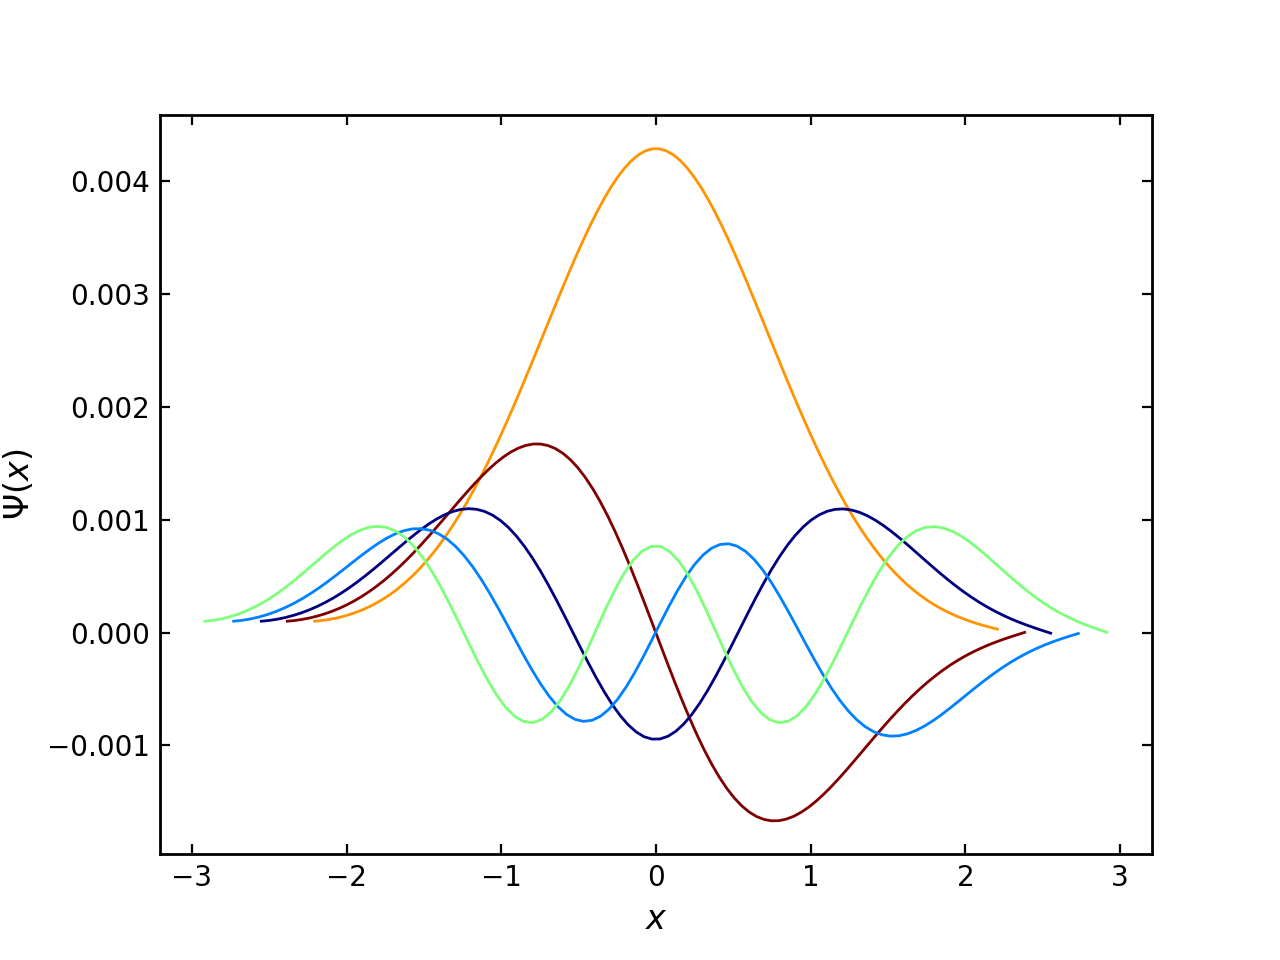
\includegraphics[height=8.5cm]{4/figs/wf_1d_exp_well_numerical}
	\vspace{0.2cm}
	\hrule
	\caption{First few eigenstates of Eqn. \eqref{1d_exp_well_SE} found numerically using a sweep over energies ($E \in [0.7, 10.0]$), $m=1$, $a = 1$, $\hbar = 1$, $k = 1$, all in atomic units.} 
	\label{wf_1d_exp_well_numerical}
\end{figure*}

Henceforth the exponential potential refers to $V(x) = k(e^{a|x|} - 1)$, which takes the same zero of energy as a PIB/particle in a sphere. The first few eigenvalues of this potential are visualised in comparison with a 1D infinite square well (PIB) with a similar functional form (\figurename{ \ref{1d_exp_well_pib_potential_eigenvalues}}). The eigenvalues are significantly more separated than those of a similar PIB. Therefore, a classical approximation of the PF may not be suitable.

\begin{figure*}[h!]

	\begin{subfigure}[t]{0.49\textwidth}
		\centering
		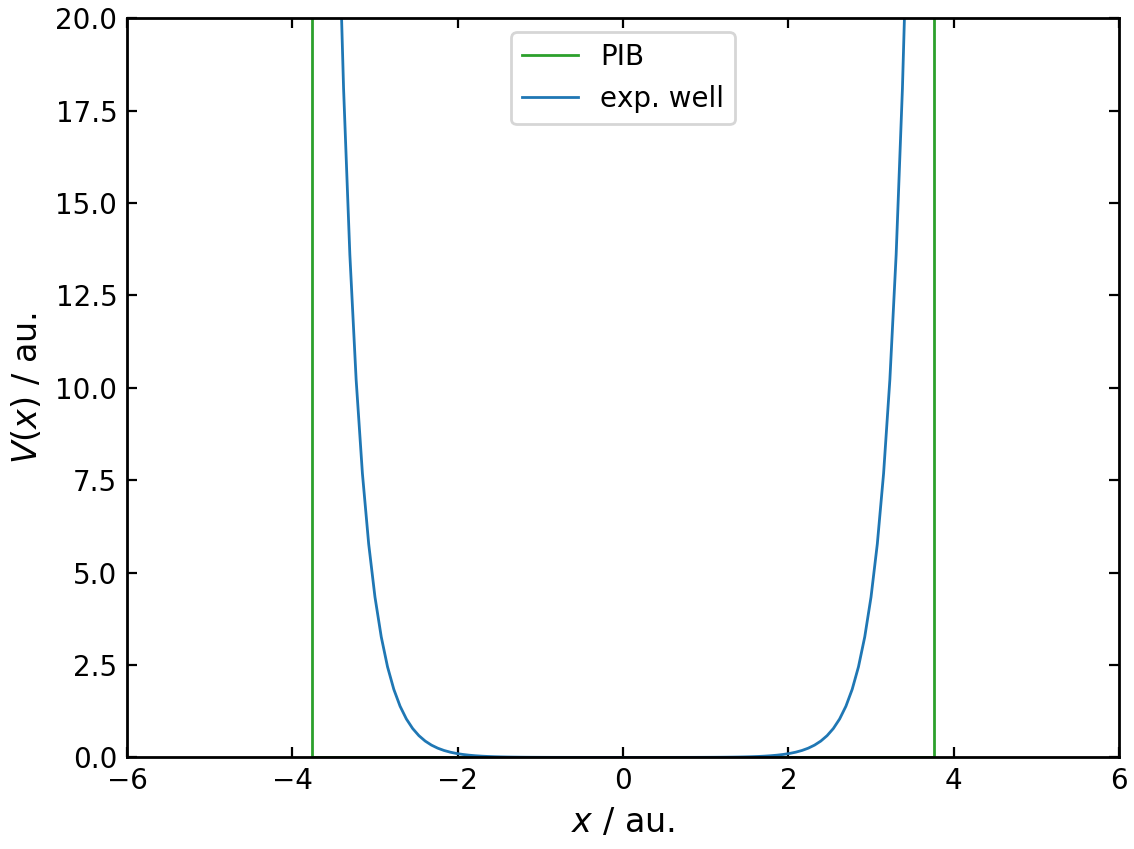
\includegraphics[height=6.2cm]{4/figs/1d_exp_well_pib_potential}
		\caption{}
	\end{subfigure}%
	~ 
	\begin{subfigure}[t]{0.49\textwidth}
		\centering
		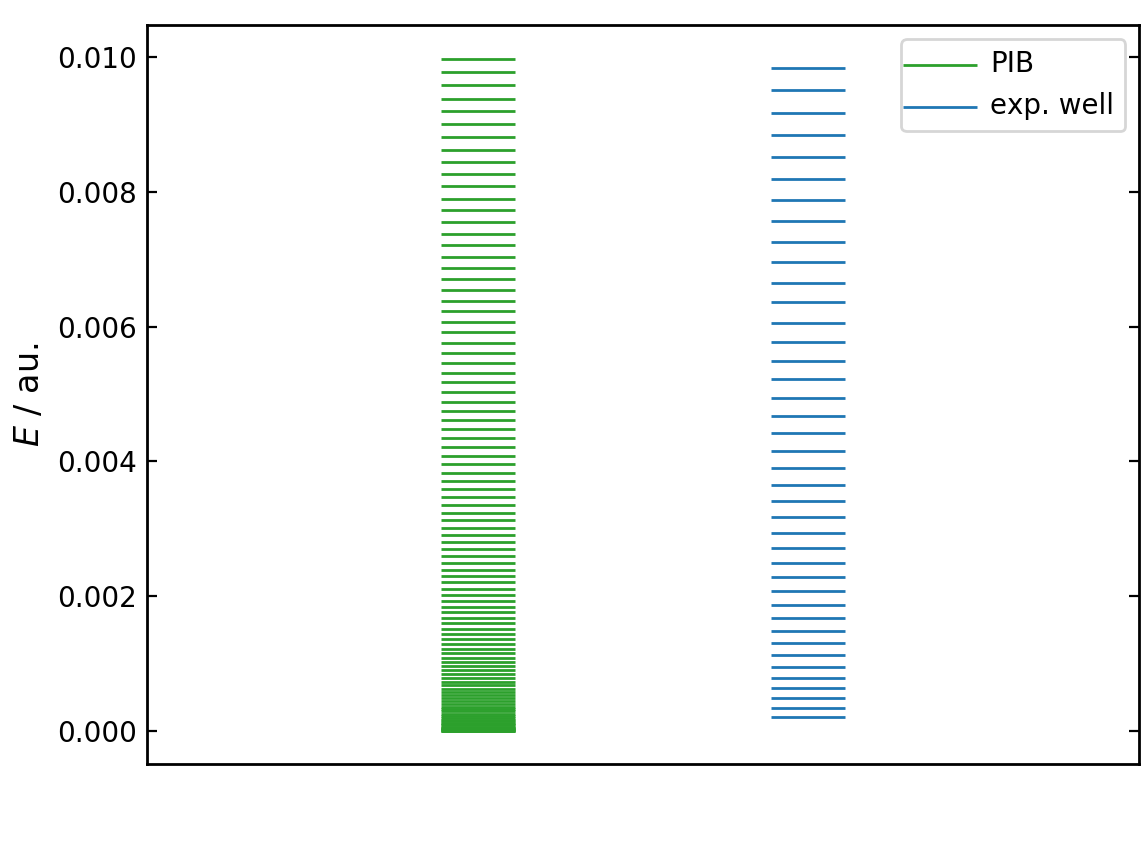
\includegraphics[height=6.2cm]{4/figs/1d_exp_well_pib_eigenvalues}
		\caption{}
	\end{subfigure}
	\vspace{0.2cm}
	\hrule
	\caption{(a) Potential energy and (b) eigenvalues ($E < 0.1$ au.) for an exponential (orange, $a = 3.0$) and infinite square well (blue, $ l = 7.52$). $\hbar = 1,\; k = 0.057 k_B T$, all in atomic units. $m =$ 48 amu.} 
	\label{1d_exp_well_pib_potential_eigenvalues}
\end{figure*}

To calculate the quantum PF only the low energy eigenstates are required. To do so requires a rapid solution of Eqn. \eqref{1d_exp_well_SE}, which is achieved using \emph{odeint} from the \emph{boost} C++ library.\cite{Ahnert2011} By sweeping energies and calculating the final value of the WF the eigenvalues may be obtained by searching for $\Psi(E, \max(x)) \ \sim 0$ i.e. a bound and normalisable solution to Eqn. \eqref{1d_exp_well_SE}. As $\Psi(E, \max(x))$ is oscillatory in $E$ the task reduces to a root finding problem (e.g. \figurename{ \ref{1d_exp_well_psi_max_vs_energy}}).

\begin{figure*}[h!]
	\centering
	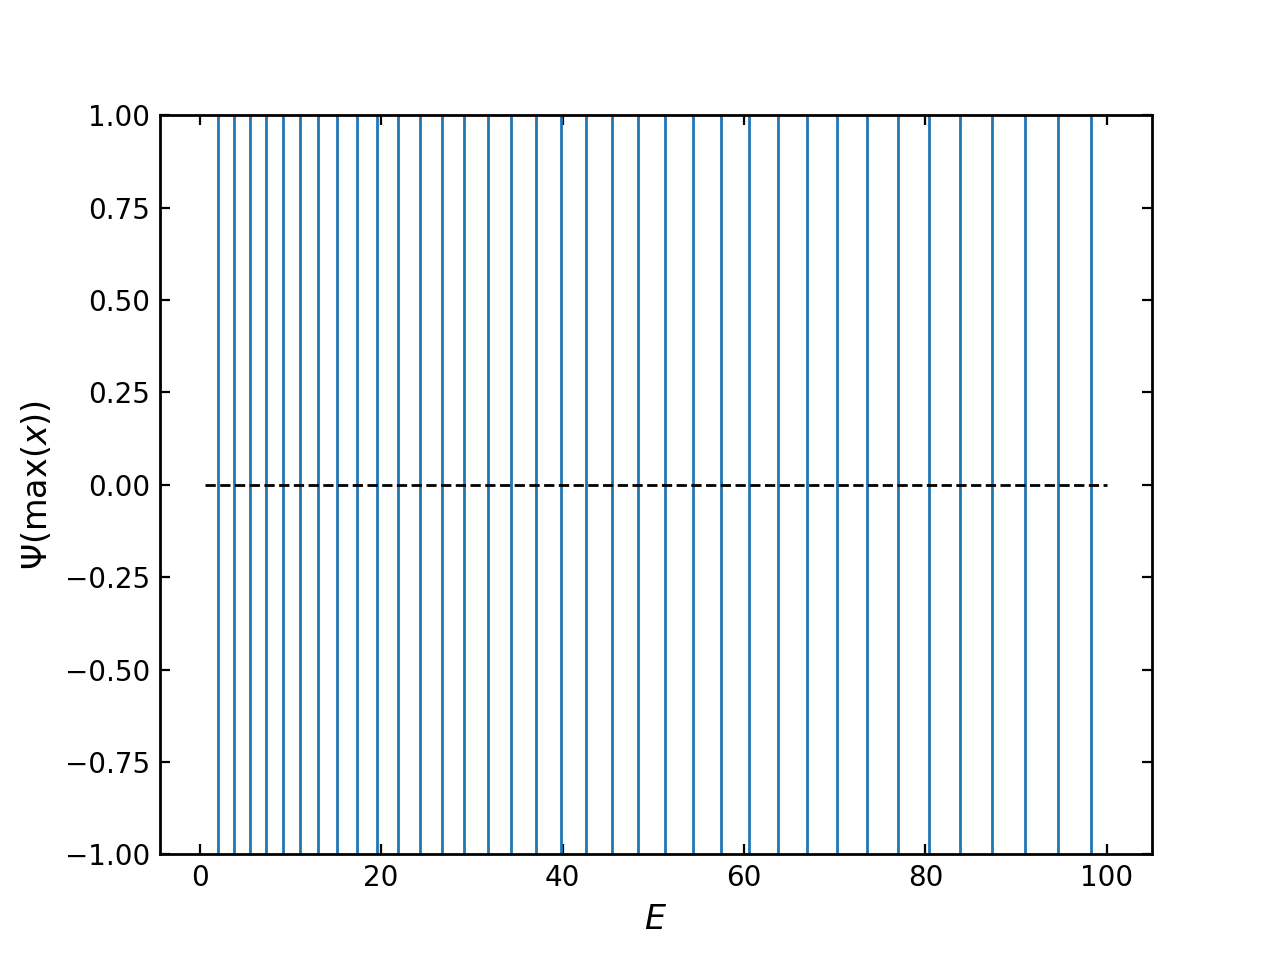
\includegraphics[height=7.2cm]{4/figs/1d_exp_well_psi_max_vs_energy}
	\vspace{0.2cm}
	\hrule
	\caption{$\Psi(E, \max(x))$ vs $E$. . $m=1, a = 1$, $\hbar = 1$ , $\max(x) = 7.5$, $x \in [-\max(x), \max(x)]$, $E \in [0.5, 100]$, $\delta E = 10^{-4}, \Psi(-\!\max(x)) = 10^{-14},\; d\Psi(x)/dx|_{-\!\max(x)} = 10^{-14}$, all in atomic units.} 
	\label{1d_exp_well_psi_max_vs_energy}
\end{figure*}
\newpage
The classical PF for the system is straightforward to derive from the classical Hamiltonian,

\begin{equation}
\mathcal{H}(p, x) = \frac{p^2}{2m} + k (e^{a|x|} - 1)
\end{equation} 
such that,
\begin{equation}
\begin{aligned}
Z_c &= \frac{1}{h}\int\int e^{-\beta \mathcal{H}(p, x)} \; dp dx \\
&=  \frac{1}{h}\int\int e^{-\beta \{{p^2}/{2m} + k e^{a|x|} - k\}} \; dp dx \\
&=  \frac{e^{\beta k}}{h}\int_{-\infty}^\infty e^{-\beta {p^2}/{2m}} \;dp \int_{-\infty}^\infty e^{-\beta k e^{a|x|}} \;  dx \\
%&=  \frac{2e^{\beta k}}{h} {\Big \{} \sqrt{\frac{\pi}{\beta / 2m}} {\Big \}}  \int_{0}^\infty e^{- \beta k e^{ax}} \;  dx \\
&=  \frac{2e^{\beta k}}{h} \cdot (2m\pi k_B T)^{1/2} \cdot \frac{1}{a} \int_{\beta k}^\infty \frac{e^{-u}}{u} \;  du \\
&=  -{\Big (} \frac{8m\pi k_B Te^{2\beta k}}{h^2a^2} {\Big )}^{1/2}  \text{Ei}(-\beta k)
\end{aligned}
\end{equation}
where the substitution $u = \beta k e^{ax}$ has been utilised and $\text{Ei}(x)$ is the exponential integral function.
\begin{figure*}[h!]
	\centering
	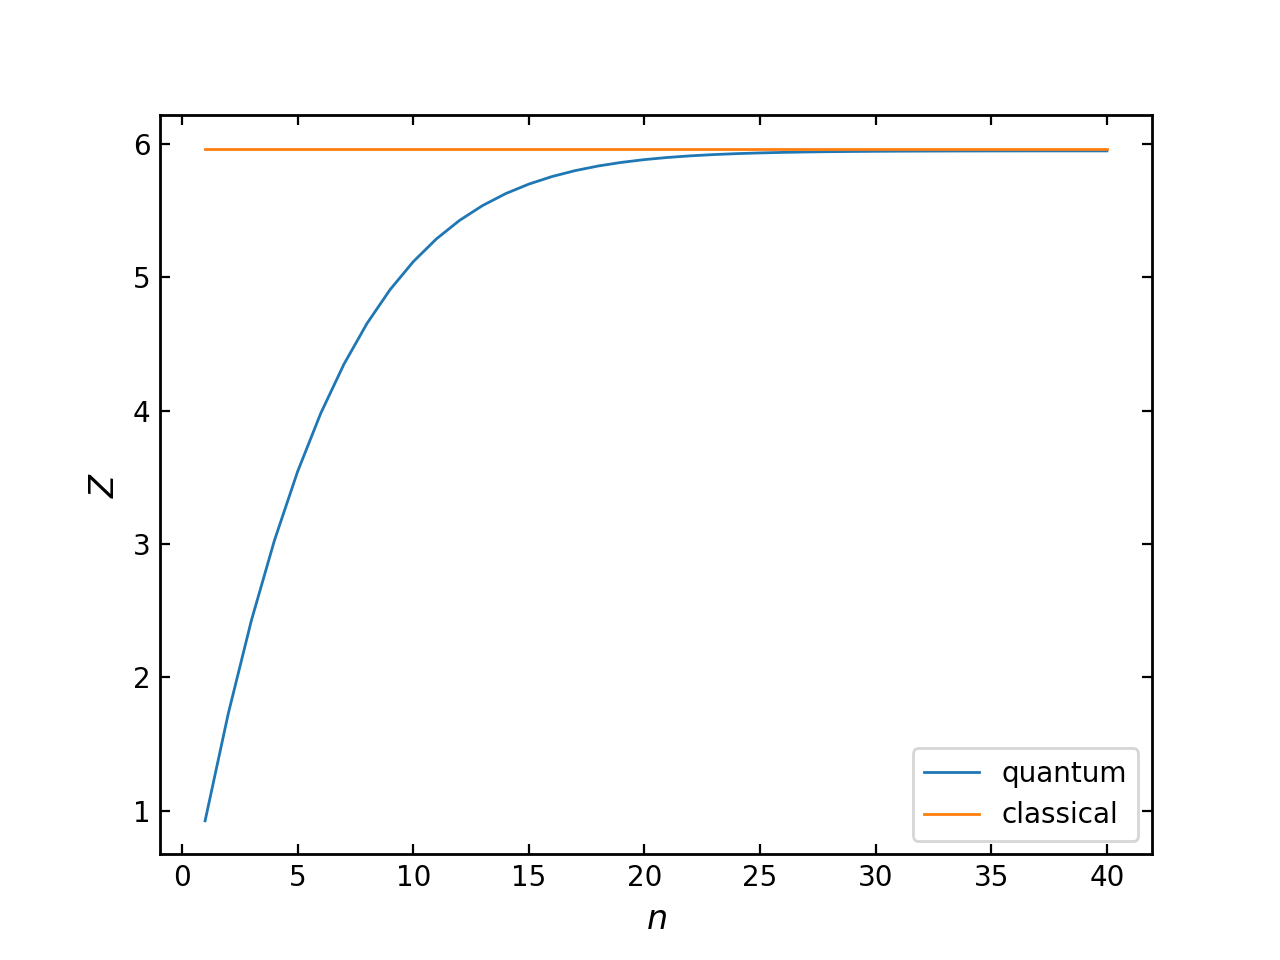
\includegraphics[height=7.5cm]{4/figs/1d_exp_well_z_qunatum_classical}
	\vspace{0.2cm}
	\hrule
	\caption{Quantum and classical PFs vs the number of eigenvalues included in the summation ($n$). $a = 3.0 \text{ au}^{-1}, k = 0.057 \; k_B T, T = 298.15 \text{ K}, m =8.75 \times 10^4$ au. Eigenvalues were found by root finding in $E= [10^{-5}, 10^{-3}]$ au with $10^4$ intermediate values. $\max(x) = 5.0, \Psi(-\!\max(x)) = 10^{-20},\; d\Psi(x)/dx|_{-\!\max(x)} = 10^{-20}$ all in au.} 
	\label{1d_exp_well_z_qunatum_classical}
\end{figure*}

For a system of mass 48 amu and a potential given in \figurename{ \ref{1d_exp_well_pib_potential_eigenvalues}a} (representative of a CO$_2$ molecule in a cavity surrounded by H$_2$O) the translational PF converges rapidly with the number of eigenvalues included in the summation (\figurename{ \ref{1d_exp_well_z_qunatum_classical}}). Despite the larger separation in eigenvalues compared to a PIB the classical approximation to the PF is still accurate ($\Delta Z_{q\rightarrow c} = 0.2\%$).

Proceeding to the 3D case the required eigenfunctions and eigenvalues are solutions of,\footnote{Where the constant shift $-k$ from setting the zero of energy is omitted as it just serves as a constant eigenvalue shift.}
\begin{equation}
\begin{aligned}
%\hat{H}\Psi(r, \theta, \phi) &= E \Psi(r, \theta, \phi) \\
{\Big \{} -\frac{1}{2m} \nabla^2 + k e^{ar} {\Big \}}\Psi(r, \theta, \phi) &= E\Psi(r, \theta, \phi) \\ 
\end{aligned}
\label{3d_exp_well_SE}
\end{equation}
where the wave function is most easily obtained in spherical coordinates for the spherical exponential well, with $r \in [0, \infty), \theta \in [0, \pi], \phi \in [0, 2\pi]$. This bears resemblance to the hydrogen atom with a modified potential in $r$. Therefore, by analogy the WF may be expressed as a product of known angular, and radial parts,
\begin{equation}
\Psi(r, \theta, \phi) = N \varphi_{l}(r) P_l^m(\cos\theta) \text{e}^{im\phi} 
\end{equation}
where the solutions are obtained from solving the radial equation with the exponential potential i.e.,
\begin{equation}
\frac{\text{d}^2\varphi_l}{\text{d} r^2} + \frac{2}{r} \frac{\text{d}\varphi_l}{\text{d}r} + \left(2m\left(E - k\text{e}^{ar}\right) - \frac{l(l+1)}{r^2}\right)\varphi_l = 0
\label{3d_exp_well_radial}
\end{equation}
where once again only a partial eigenspecturm is required so solving Eqn. \eqref{3d_exp_well_radial} numerically over possible $l$ ($l \in \mathbb{Z}_{\ge0}$) at fixed $a, k$ should be sufficient. In a similar vein to the 1D case Eqn. \eqref{3d_exp_well_radial} may be solved numerically by ensuring $\varphi_r(r) \rightarrow 0$ as $r \rightarrow \infty$ as the potential diverges and $\varphi_r(0) \in \mathbb{R}$, so the WF is normalisable. Noting that the ODE diverges at $r = 0$ and will lead to numerical instabilities, the first few eigenfunctions are shown in \figurename{ \ref{fig::entropy_X6}}b, found by sweeping energies and selecting normalisable functions. Propagating away from the centre of the potential (forwards) again $\varphi_r(r=r_\text{max})$ oscillates between $\pm \infty$ in $E$, thus the eigenvalue is taken between where $\varphi_r(r_\text{max})$ changes sign. An almost identical eigenvalue ($\Delta E < 0.01$ cm$^{-1}$) is obtained when $\varphi(0) \nrightarrow \pm \infty$, with an eigenfunction that resembles a 1s orbital (\figurename{ \ref{fig::entropy_X6}a}). Obtaining higher lying eigenstates is then straightforward, with the first few shown in  \figurename{ \ref{fig::entropy_X6}b}. In contrast to the hydrogen atom, the potential does not admit any higher symmetries to afford degeneracy between $l$ levels, despite the eigenfunctions being qualitatively similar to the hydrogen radial wave functions. The $2l + 1$ degeneracy in the magnetic quantum number is retained due to the identical radial component. 
% https://en.wikipedia.org/wiki/Laplace–Runge–Lenz_vector#CITEREFHall2013
% https://users.aber.ac.uk/ruw/teach/327/hatom.php
\vspace{0.2cm}
\begin{figure*}[h!]
	\begin{subfigure}[t]{0.5\textwidth}
		\centering
		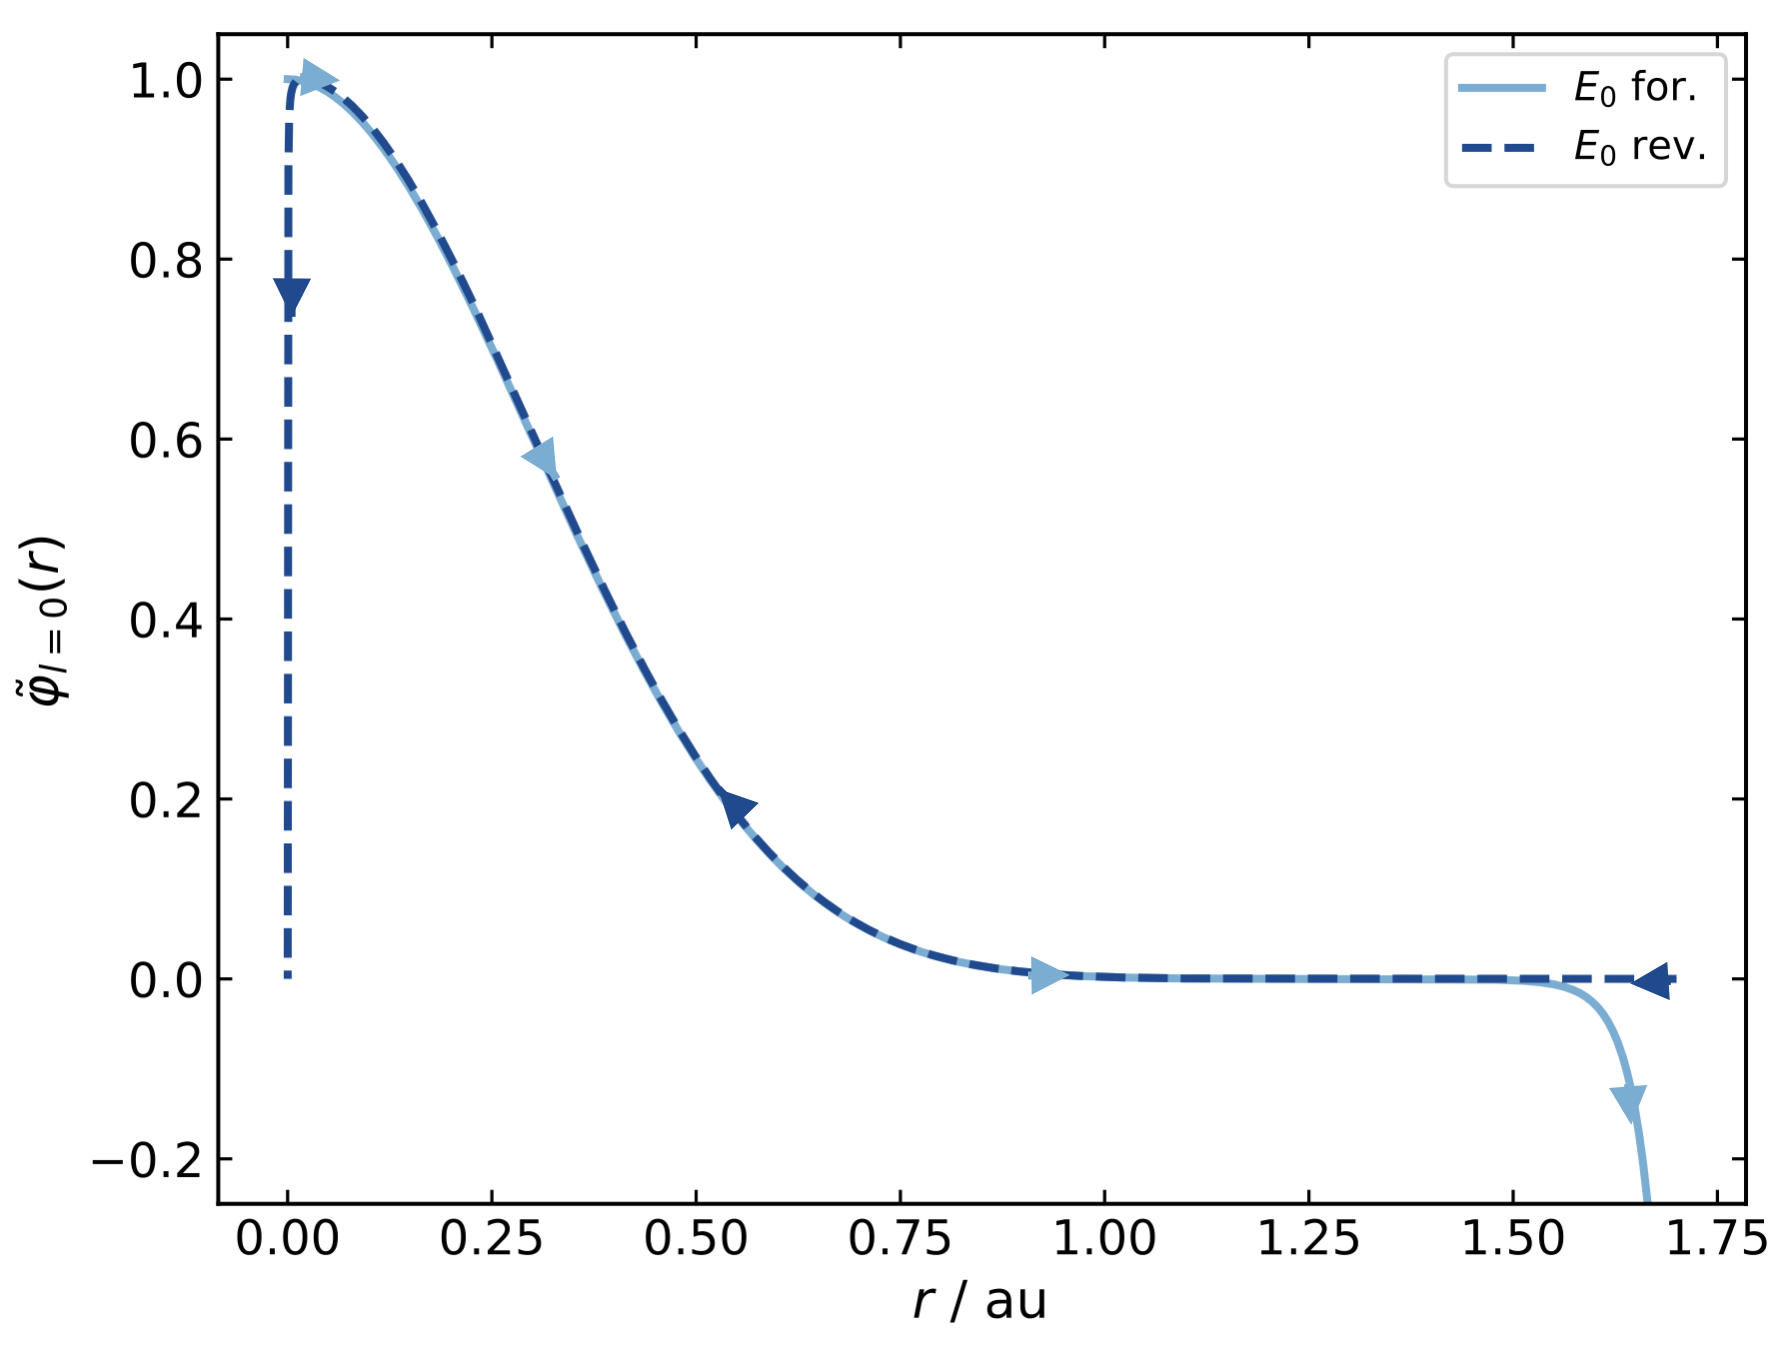
\includegraphics[height=6.2cm]{4/figs/figX6/first_eigenfunction_lines.png}
		\caption{}
	\end{subfigure}%
	~ 
	\begin{subfigure}[t]{0.5\textwidth}
		\centering
		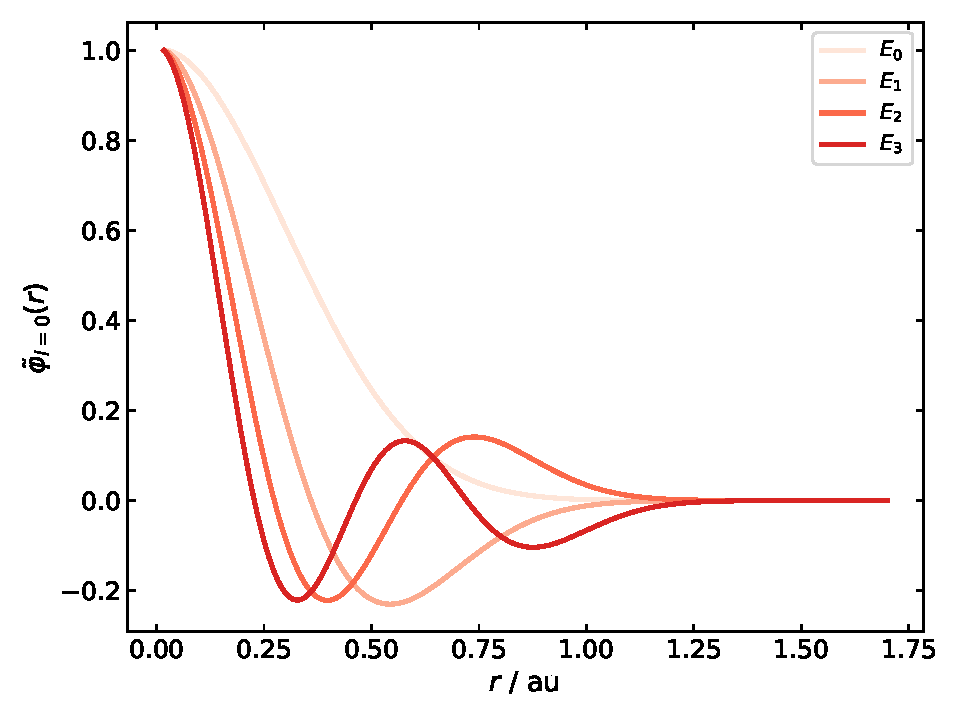
\includegraphics[height=6.2cm]{4/figs/figX6/eigenfunctions.pdf}
		\caption{}
	\end{subfigure}
	\vspace{0.2cm}
	\hrule
	\caption{Numerical solution of Eqn. \eqref{3d_exp_well_radial} for (a) the lowest energy eigenvalue $E_0$ located by propagating forwards and in reverse from $r = \delta : \delta \ll 1$ and (b) the lowest four eigenvalues where $\varphi$ is normalised to 1 at $\delta$ for clarity. $m =8.75 \times 10^4$,$k = 5.47 \times 10^{-5}$, $a = 3.0$, using $r_\text{max} = 1.7$, $l = 0$. All quantities in atomic units.} 
	\label{fig::entropy_X6}
\end{figure*}

The partial eigenspecturm is obtained as above and reasonably efficiently (execution time $\sim1$ min), from which summation over states converges reasonably to the classical result for CO$_2$ in water (\figurename{ \ref{fig::entropy_X7}a}), and is within 1 \% for a limiting case (\figurename{ \ref{fig::entropy_X7}b}) at a lower temperature.\footnote{A reduced temperature ($T$ = 50 K) is used in this system to limit the number of  eigenvalues required to converge the quantum PF. The quantum--classical correspondence is expected to be even more exact at larger higher temperatures.}. This convergence is expected given as the dimensionality of a system increases, it becomes more classical in nature (\emph{cf.} the quantum-classical correspondence in the limit of infinite spacial dimensions).\cite{QuantClassCorrespondence}. Noting that the entropy depends on the log of the PF this suggests the classical approximation will be sufficient.

\vspace{0.2cm}
\begin{figure*}[h!]
	\begin{subfigure}[t]{0.5\textwidth}
		\centering
		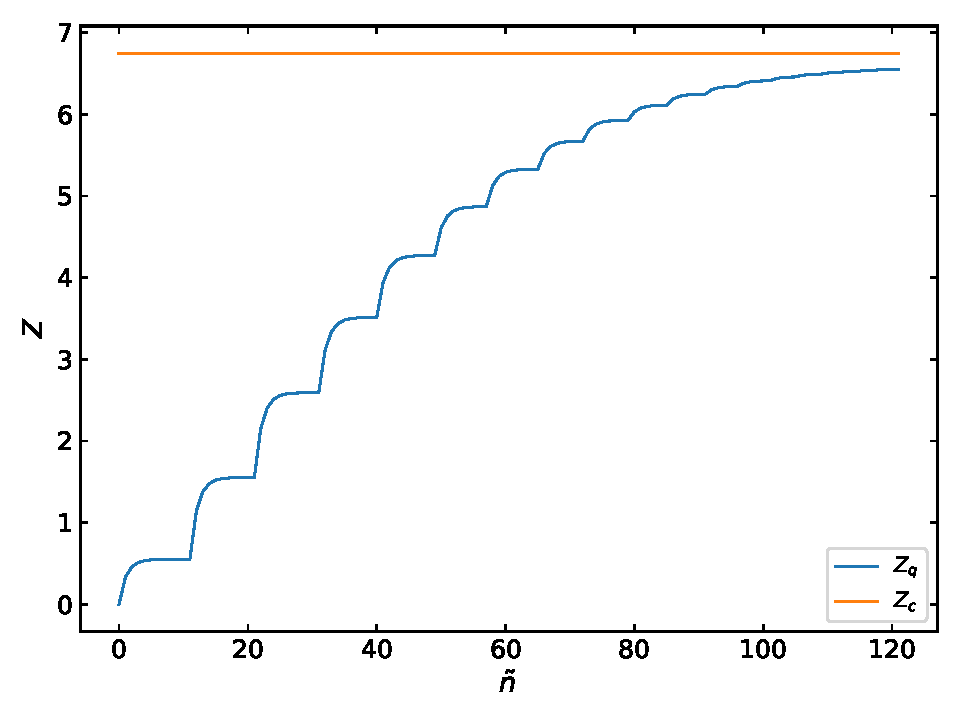
\includegraphics[height=6.2cm]{4/figs/figX7/quantum_classical_comparison_co2.pdf}
		\caption{}
	\end{subfigure}%
	~ 
	\begin{subfigure}[t]{0.5\textwidth}
		\centering
		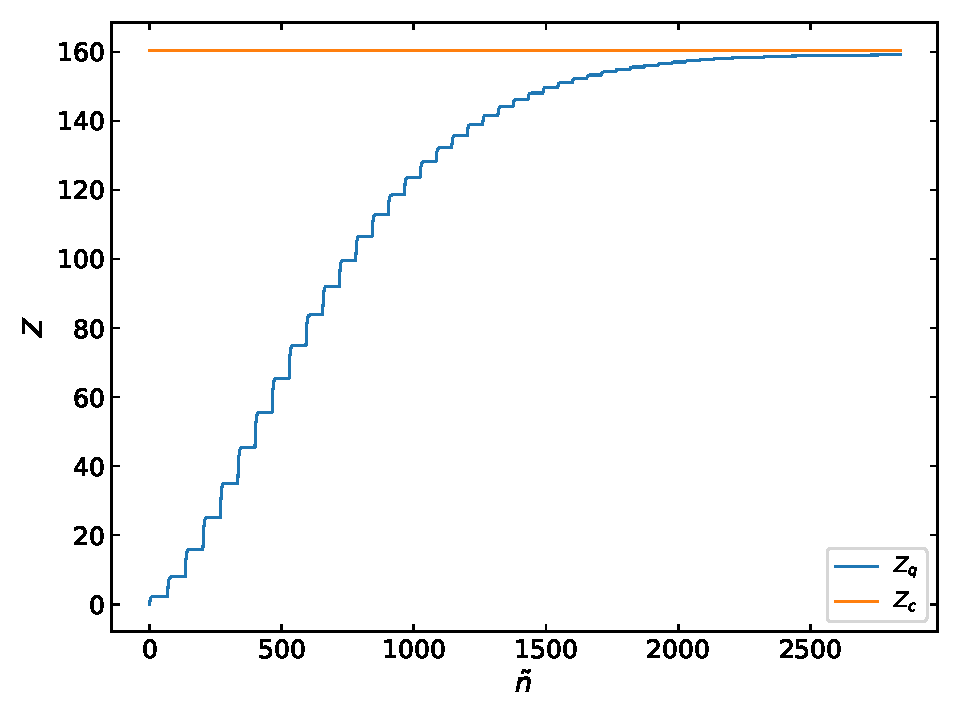
\includegraphics[height=6.2cm]{4/figs/figX7/quantum_classical_comparison_limiting.pdf}
		\caption{}
	\end{subfigure}
	\vspace{0.2cm}
	\hrule
	\caption{Quantum ($Z_q$) and classical ($Z_c$) partition functions for a 3D EW as a function of number of included eigenvalues ($\tilde{n}$) for (a) CO$_2$ in water ($a = 1.499$, $k=0.00221$, $m=8.75 \times 10^4$, $k_BT = 9.437 \times 10^{-4}$) and (b) a limiting case ($a = 1.499$, $k=1\times 10^{-4}$, $m=8.75 \times 10^5$, $k_BT = 1.583 \times 10^{-4}$). Eigenvalues located using a numerical solution of Eqn. \eqref{3d_exp_well_radial} by iterating through $E \in [1\times10^{-5}, 10 k_BT]$ in 20,000 steps with integer $l \in [0, 50]$ from $r = 1\times10^{-3}$ to $r_\text{max} = 1.7$. All quantities in atomic units. 
	} 
	\label{fig::entropy_X7}
\end{figure*}

The classical PF is straightforwardly
\begin{equation}
\begin{aligned}
Z_c^\text{exp} &= \frac{1}{h^3}\int\int e^{-\beta \mathcal{H}(\boldsymbol{p}, \boldsymbol{r})} \; d\boldsymbol{p} d\boldsymbol{r} \\
&=  \frac{1}{h^3} (2m\pi k_B T)^{3/2}  \int_{-\infty}^\infty e^{\beta k}e^{-\beta k e^{a|\boldsymbol{r}|}} \;  d\boldsymbol{r} \\
&=   e^{\beta k}{\Big (} \frac{2m\pi k_B T}{h^2} {\Big )}^{3/2}  \int_{0}^\infty e^{-\beta k e^{a{r}}} 4\pi r^2\;  d{r} \\
&=  4\pi  e^{\beta k}{\Big (} \frac{2m\pi k_B T}{h^2} {\Big )}^{3/2}  \int_{0}^\infty r^2 e^{-\beta k e^{a{r}}} \;  d{r}
\end{aligned}
\label{z_classical_exp_well}
\end{equation}

where the integral is non-analytic, and thus must be evaluated numerically, but is smooth and well localised around 0 (\figurename{ \ref{fig::entropy_X8}}a), making a numerical solution possible. However, from Eqn. \eqref{z_classical_exp_well} the integrand is exponential in $k$ and super-exponential in $a$ making the $Z_c$ dependence significant (logarithmic, \figurename{ \ref{fig::entropy_X8}}b). Here it is worth noting that the dominant contribution to the integral is for $V < 10k_B T$, making fits up to a 100 \kcal $\,$ maximum non-optimal when the integrand is zero above $V \sim 5$ \kcal. Instead, the fit should be focused in the low-energy regions for optimal accuracy.

\vspace{0.2cm}
\begin{figure*}[h!]
	\begin{subfigure}[t]{0.5\textwidth}
		\centering
		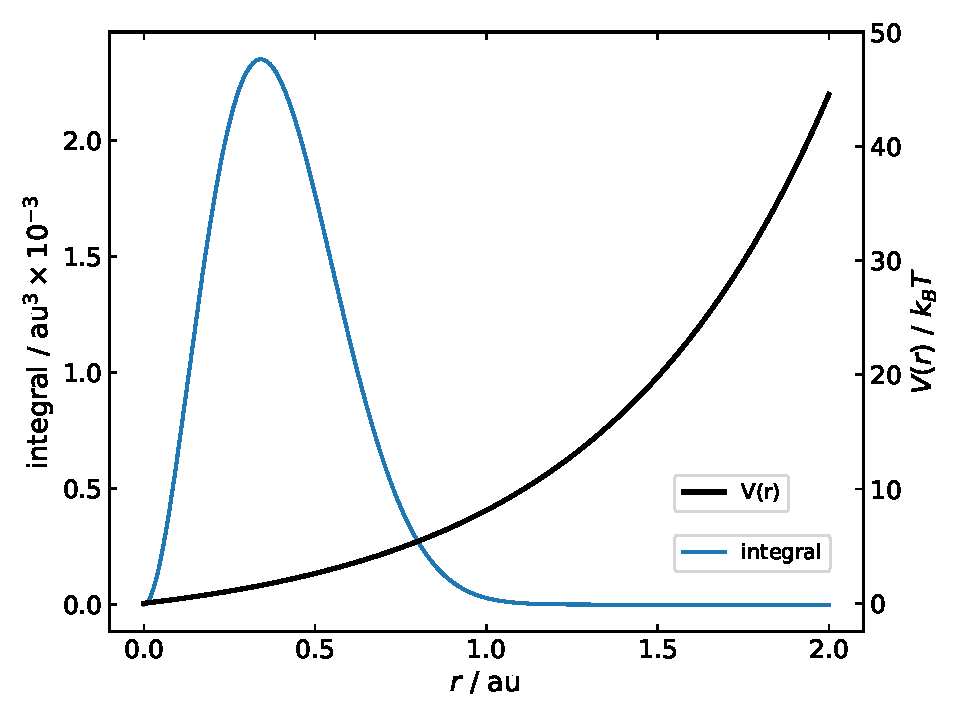
\includegraphics[height=6.2cm]{4/figs/figX8/classical_integrand.pdf}
		\caption{}
	\end{subfigure}%
	~ 
	\begin{subfigure}[t]{0.5\textwidth}
		\centering
		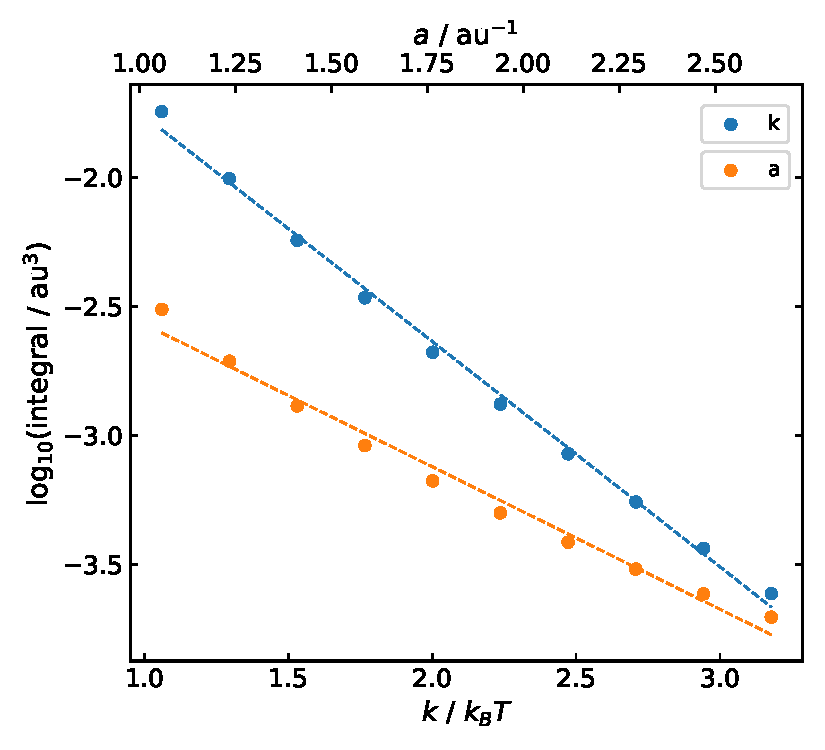
\includegraphics[height=6.7cm]{4/figs/figX8/integrand_a_k.pdf}
		\caption{}
	\end{subfigure}
	\vspace{0.2cm}
	\hrule
	\caption{(a) Integrand from Eqn. \eqref{z_classical_exp_well} and potential $V(r) = k(e^{ar} - 1)$, and (b) dependence of the integrand on $k$ and $a$. Parameters as \figurename{ \ref{fig::entropy_X7}a} with all quantities in atomic units.} 
	\label{fig::entropy_X8}
\end{figure*}

The corresponding entropy for a molecule confined to an EW can be derived from the PF Eqn. \eqref{z_classical_exp_well} as,
\begin{equation}
S_\text{trans}^\text{exp}= k_B {\Big (} \frac{3}{2} - {k}{\beta} + \ln(Z_c^\text{exp}) + \frac{4\pi k\beta\Lambda}{Z_c^\text{exp}} \int_{0}^{\infty} r^2 e^{ar} e^{-\beta k (e^{ar} - 1)} \; \text{d}r  {\Big )} 
\label{s_ew}
\end{equation}

where $\Lambda = (2m\pi/\beta h^2)^{3/2}$ and the temperature derivative of the PF is shown in Appendix \ref{section::appendix_igm_partition_functions}. The associated internal energy is then,

\begin{equation}
\begin{aligned}
E_\text{trans}^\text{exp} &= k_BT^2 \left(\frac{\partial \ln Z_c^\text{exp}}{\partial T} \right)_{N, V}  \\
&= \frac{k_BT^2}{Z_c^\text{exp}} \left(\frac{\partial Z_c^\text{exp}}{\partial T} \right)_{N, V} \\
&=\frac{3k_BT}{2} - k + \frac{4 \pi k \Lambda}{Z_c^\text{exp}} \int_0^\infty r^2 e^{ar} e^{-\beta k (e^{ar} - 1)} \;\text{d}r
\end{aligned}
\label{E_ew}
\end{equation}

which reproduces the correct equipartition limit as $k \rightarrow 0$, and likewise as $a$ vanishes, again $E_\text{trans}^\text{exp} \rightarrow 3k_BT/2$.

Regenerating surfaces over a narrower energy window generates more accurate parameters and translational entropies that are around one half (43 $\pm$ 2 \%) of their PIB analogues (at a 1 M effective volume) and provide a theoretical basis for sub-unity scalings proposed in refs. \cite{Tanaka2011, Deubel2006, Li2016, DiTommaso2010}. As expected, and in contrast to the IGM, the EW recovers a solvent dependence on the  translational entropy (and energy, from Eqn. \eqref{E_ew}) which should be present. For higher number density solvents e.g. water that are more tightly packed around the solute, the translational entropy is uniformly smaller than for acetonitrile or benzene, as would be expected.
\vspace{0.2cm}

\begin{table}[h!]
	\renewcommand{\arraystretch}{1.5}
	\begin{center}
		\small
		\begin{tabularx}{\textwidth}{YYYYYYY} 
			\toprule
			Solute & Solvent& $k$ / \kcal & $a$ / \AA$^{-1}$ & $TS_\text{trans}^\text{PIB, 1 atm}$ &  $TS_\text{trans}^\text{PIB, 1 M}$ & $TS_\text{trans}^\text{exp}$ \\
			\hline
			% From fits up to 100 kcal mol1
		%	Methane  & Water &   1.278    &   2.705     \\
		%	Methane  & Acetonitrile &   0.718    &   2.500    \\
		%	Methane  & Benzene &   0.911    &    2.449    \\
		%	CO$_2$  & Water&   1.386    &    2.832     \\
		%	CO$_2$  & Acetonitrile&   0.655    &    2.562   \\
		%	CO$_2$  & Benzene &    0.707   &    2.809   \\
		%	Alanine   &Water &     1.692  &    2.688     \\
		%	Alanine   & Acetonitrile&   0.796    &    2.473   \\
		%	Alanine   & Benzene &   0.524   &   2.542    \\
			
			Methane  & Water & 1.048 & 2.918& 9.623  &  7.729  &  2.5 \\
			Methane  & Acetonitrile & 0.529 & 2.793 & 9.623  &  7.729  &  3.162\\
			Methane  & Benzene & 0.679& 2.736 &9.623  &  7.729  &  2.997\\
			CO$_2$  & Water&  0.545 & 4.075 &10.52  &  8.626  &  3.364\\
			CO$_2$  & Acetonitrile& 0.446& 2.930 &10.52  &  8.626  &  4.104\\
			CO$_2$  & Benzene & 0.415 &3.431 &10.52  &  8.626  &  3.877\\
			Alanine   &Water & 0.53 & 4.083 &11.147  &  9.252  &  4.009\\
			Alanine   & Acetonitrile&1.005 & 2.127 &11.147  &  9.252  &  4.625\\
			Alanine   & Benzene & 0.368 & 2.878 &11.147  &  9.252  &  4.903\\
			% Average && 1.0 ± 0.4 & 2.6 ± 0.1 \\
			\bottomrule
		\end{tabularx}
	\end{center}
	\caption{Fitted parameters for exponential wells for different solute-solvent systems at the DFTB//XTB level of theory Fits performed over the [0, 10] \kcalx energy window on $\sim 10$ points for average potentials (500 points) with $x \in [-1, 1]$ \AA. $T = 298.15$ K.} 
	\label{table::figX9_params}
\end{table}


\subsection{Test Cases}

With a new method to calculate the translational entropy experimental validation is required. Two benchmark sets that comprise accurate activation and reaction entropies were selected (Appendix \ref{section::appendix_entropy_test_cases}). Calculating IGM entropy differences reveals they are subject to a reasonably systematic shift using a 1 M effective volume (\figurename{ \ref{fig::entropy_X10}}). Both the entropies of reaction (blue, \figurename{ \ref{fig::entropy_X10}}) and activation (red, \figurename{ \ref{fig::entropy_X10}}) are bimolecular and therefore do not have a vanishing translational entropy contribution. Introducing an EW treatment of the translational entropy reduces the error to experimental values by some 3 \kcal, while also including an error that almost always encompasses the correct value (at 1$\sigma$). This error arises from an average model generated using $\bar{k}, \bar{a}$ parameters (from \tablename{ \ref{table::figX9_params}}), their associated standard deviations and propagating the assumed uncorrelated errors through to $\Delta S$. 

\vspace{0.3cm}
\begin{figure*}[h!]
	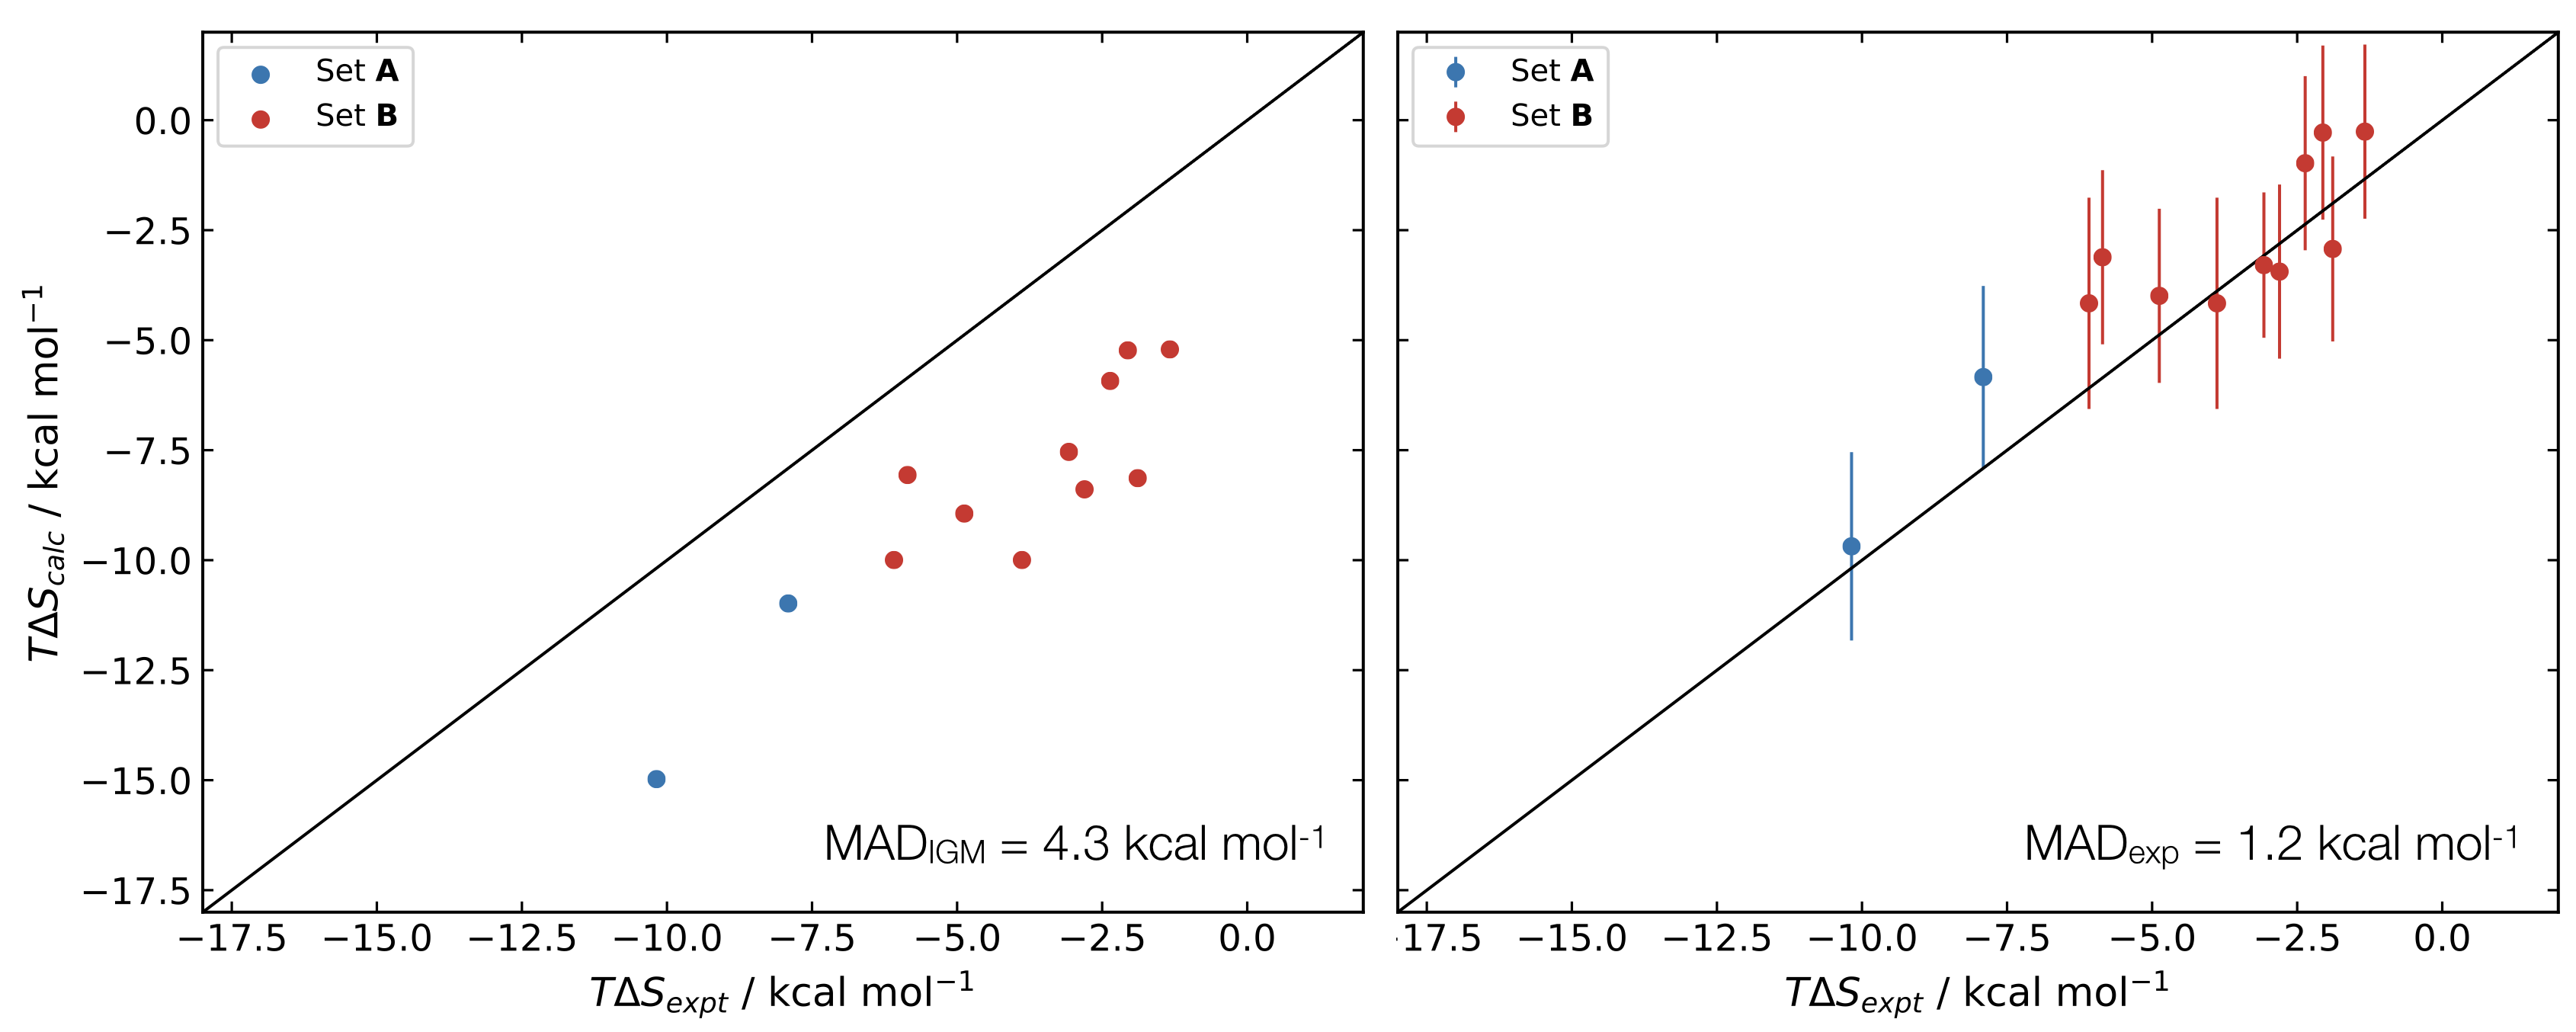
\includegraphics[width=\textwidth]{4/figs/figX10/figX10}
	\vspace{0.2cm}
	\hrule
	\caption{Correlation between calculated and experimental entropy contributions to the free energy for test sets {\bfseries{A, B}}, shown in Appendix \ref{section::appendix_entropy_test_cases}. Left are ideal gas values (1 M) and right EW generated from an average model and $1\sigma$ errors plotted from standard deviations in $k, a$.} 
	\label{fig::entropy_X10}
\end{figure*}

Once again, the solvent reorganisation entropy is not included in the calculated values as it is parametrised into the implicit solvent models. Although the overall solvent reorganisation free energy for a reaction is thought to cancel exactly, the environmental $\Delta H_\text{env}, T\Delta S_\text{env}$ terms may be significant (up to $\sim 10\;$\kcal, with opposing signs).\cite{Grunwald1995}
However, a recent literature review of protein-ligand binding found little entropy-enthalpy compensation suggesting a system dependence.\cite{Chodera2013} Here, it would seem surprising if the solvent reorganisation entropy were to cause such a systematic shift given the diversity of solvents (methanol, dimethyl-formamide, acetonitrile, dimethyl-sulfoxide) suggesting that the origin lies in the intrinsic translational contribution. Using the EW approximation to the translational entropy here increases the absolute accuracy over the standard IGM treatment and provides a quantification of the likely error. 
\\\\
Moving to the striking case of water-in-water presented above, which illustrated the limitation of the IGM, an EW corrects almost all of the IGM deficiencies and affords a free energy difference close to zero (\figurename{ \ref{fig::etropy_X11}}). The agreement is somewhat surprising given (1) the SMD solvent model is parametrised to the IGM, (2) the rotational contribution remains at the rigid rotor level and (3) an average EW model is used. Explanations for some of these points are given in the following.
\\
Free energy differences for the (H$_2$O)$_8 \longrightarrow$ (H$_2$O)$_7$ +  H$_2$O identity reaction using an EW may be calculated in two ways (blues, \figurename{ \ref{fig::entropy_X11}}); either treating the translation of one molecule within the octamer and the separated components [(H$_2$O)$_8$, (H$_2$O)$_7$, H$_2$O] using an EW,  and deleting three low frequency modes approximately corresponding to translation (exp$_1$), or just modifying (PIB$\rightarrow$EW) the translational entropy and internal energy of each whole component  (exp$_2$). Interestingly, these two methods lead to an almost identical free energy change $\sim 0$. This is due to the vibrational entropy (treated as mostly rotation within the qRRHO with frequencies $< 50$ cm$^{-1}$) matching the EW translational entropy ($\sim 3\;$\kcal, at this temperature). 
\vspace{0.4cm}
\begin{figure*}[h!]
	\centering
	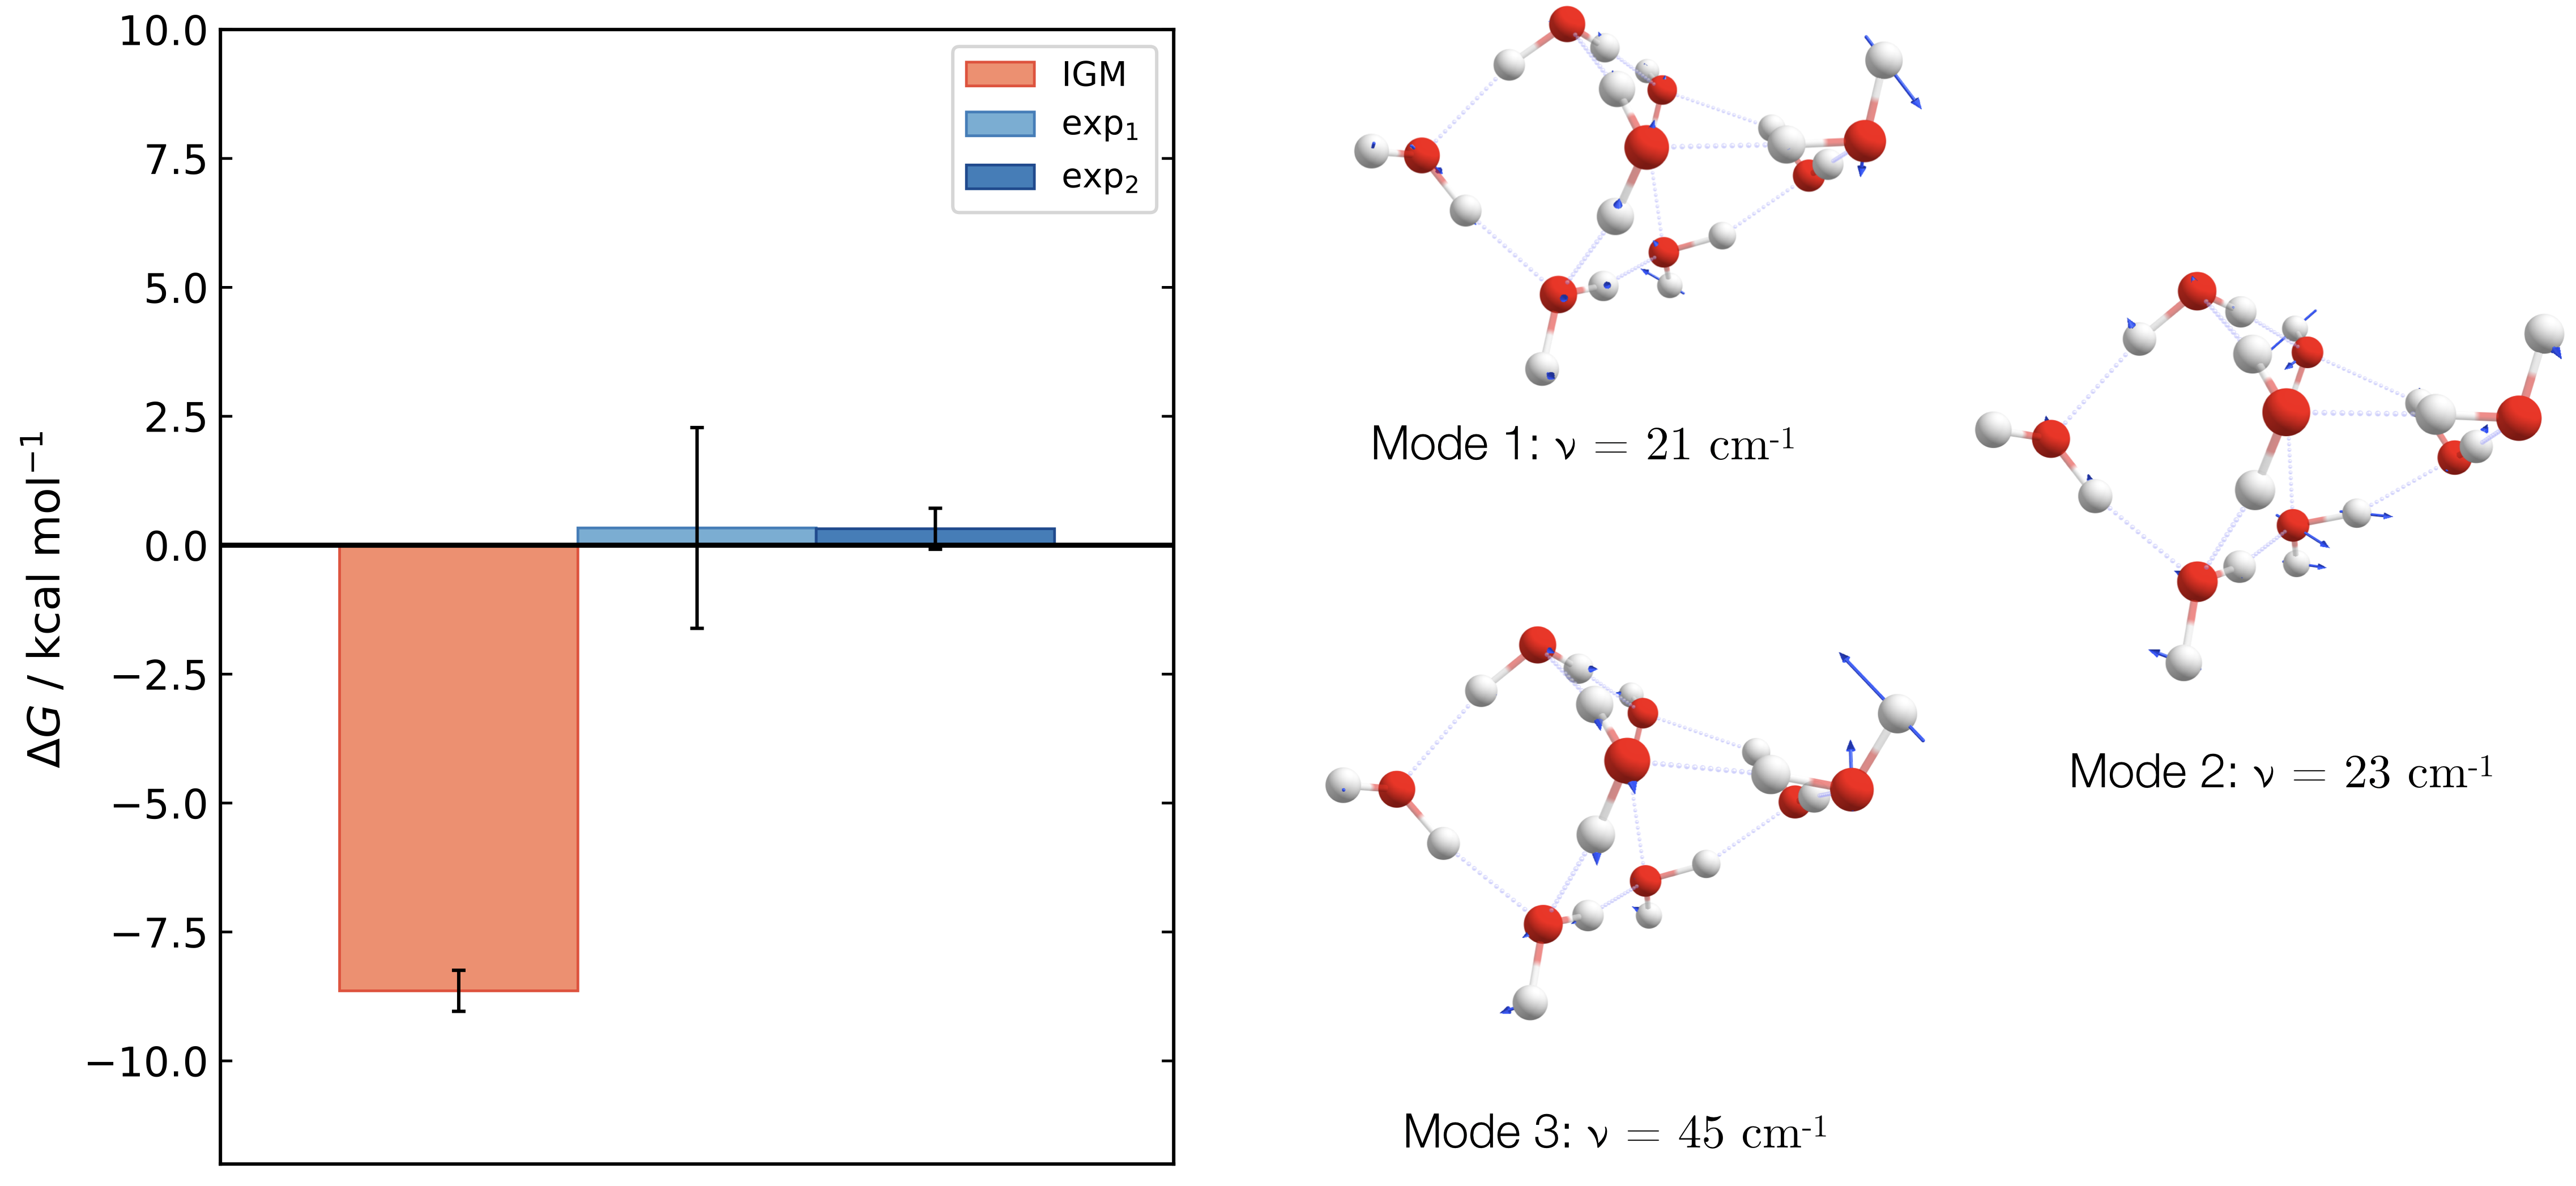
\includegraphics[width=15cm]{4/figs/figX11/figX11}
	\vspace{0.2cm}
	\hrule
	\caption{Comparison of ideal gas (qRRHO) and ideal gas with a EW treatment of the translational entropy free energy changes for the (H$_2$O)$_8 \longrightarrow$ (H$_2$O)$_7$ +  H$_2$O identity reaction in implicit (SMD) water. The three lowest energy modes corresponding to overall translational modes treated with an EW rather than a harmonic oscillator approximation for the water (H$_2$O)$_8$ are also shown.} 
	\label{fig::entropy_X11}
\end{figure*}

While the SMD implicit solvent model has been parametrised to IGM solvation free energies, water clusters are absent from the test set,\cite{Marenich2009} making the large discrepancy less surprising. Furthermore, while the treatment of the rotational contribution to the entropy and internal energy changes when dissociating a water molecule from a cluster the absolute magnitude is small ($TS_\text{rot}^{\text{H}{}_2\text{O}} =$ 3.2 \kcal) and is compensated on the left-hand side of the reaction by the vibrational modes that are mostly treated as rotations. Finally, using an average model leads to a larger error for exp$_1$ value, but encompasses the correct value; while, in exp$_1$ the translational component broadly cancels.

\newpage
Finally, host-guest binding affinity calculations performed in Chapter 3 may now be re-evaluated with this new methodology.  A set of binding entropy changes are available in the literature,\cite{Leung2008} the systems comprise more than 300 atoms, making accurate DFT calculations (hybrid, with Hessians) prohibitively expensive. Therefore, the [Pd$_2$L$_4$]${}^{2+}$ systems ($\sim140$ atoms) investigated in ref. \cite{Young2019} will form a test set to calculate binding free energies using an EW approximation. Scaling the translational entropy down with an average EW approximation leads to excellent agreement to experiment where low frequency modes are treated as rotors (qRRHO, \figurename{ \ref{fig::entropy_X12}}), in contrast to the standard IGM. This suggests that, again, the EW provides improved accuracy while being more theoretically justified.\footnote{There, however, remains a significant functional dependence on $\Delta E_\text{bind, calc}$ of $\sim 5$ \kcal, and higher level coupled cluster calculations are not routinely possible for a system with $\sim 150$ atoms.}

\vspace{0.4cm}
\begin{figure*}[h!]
	\centering
	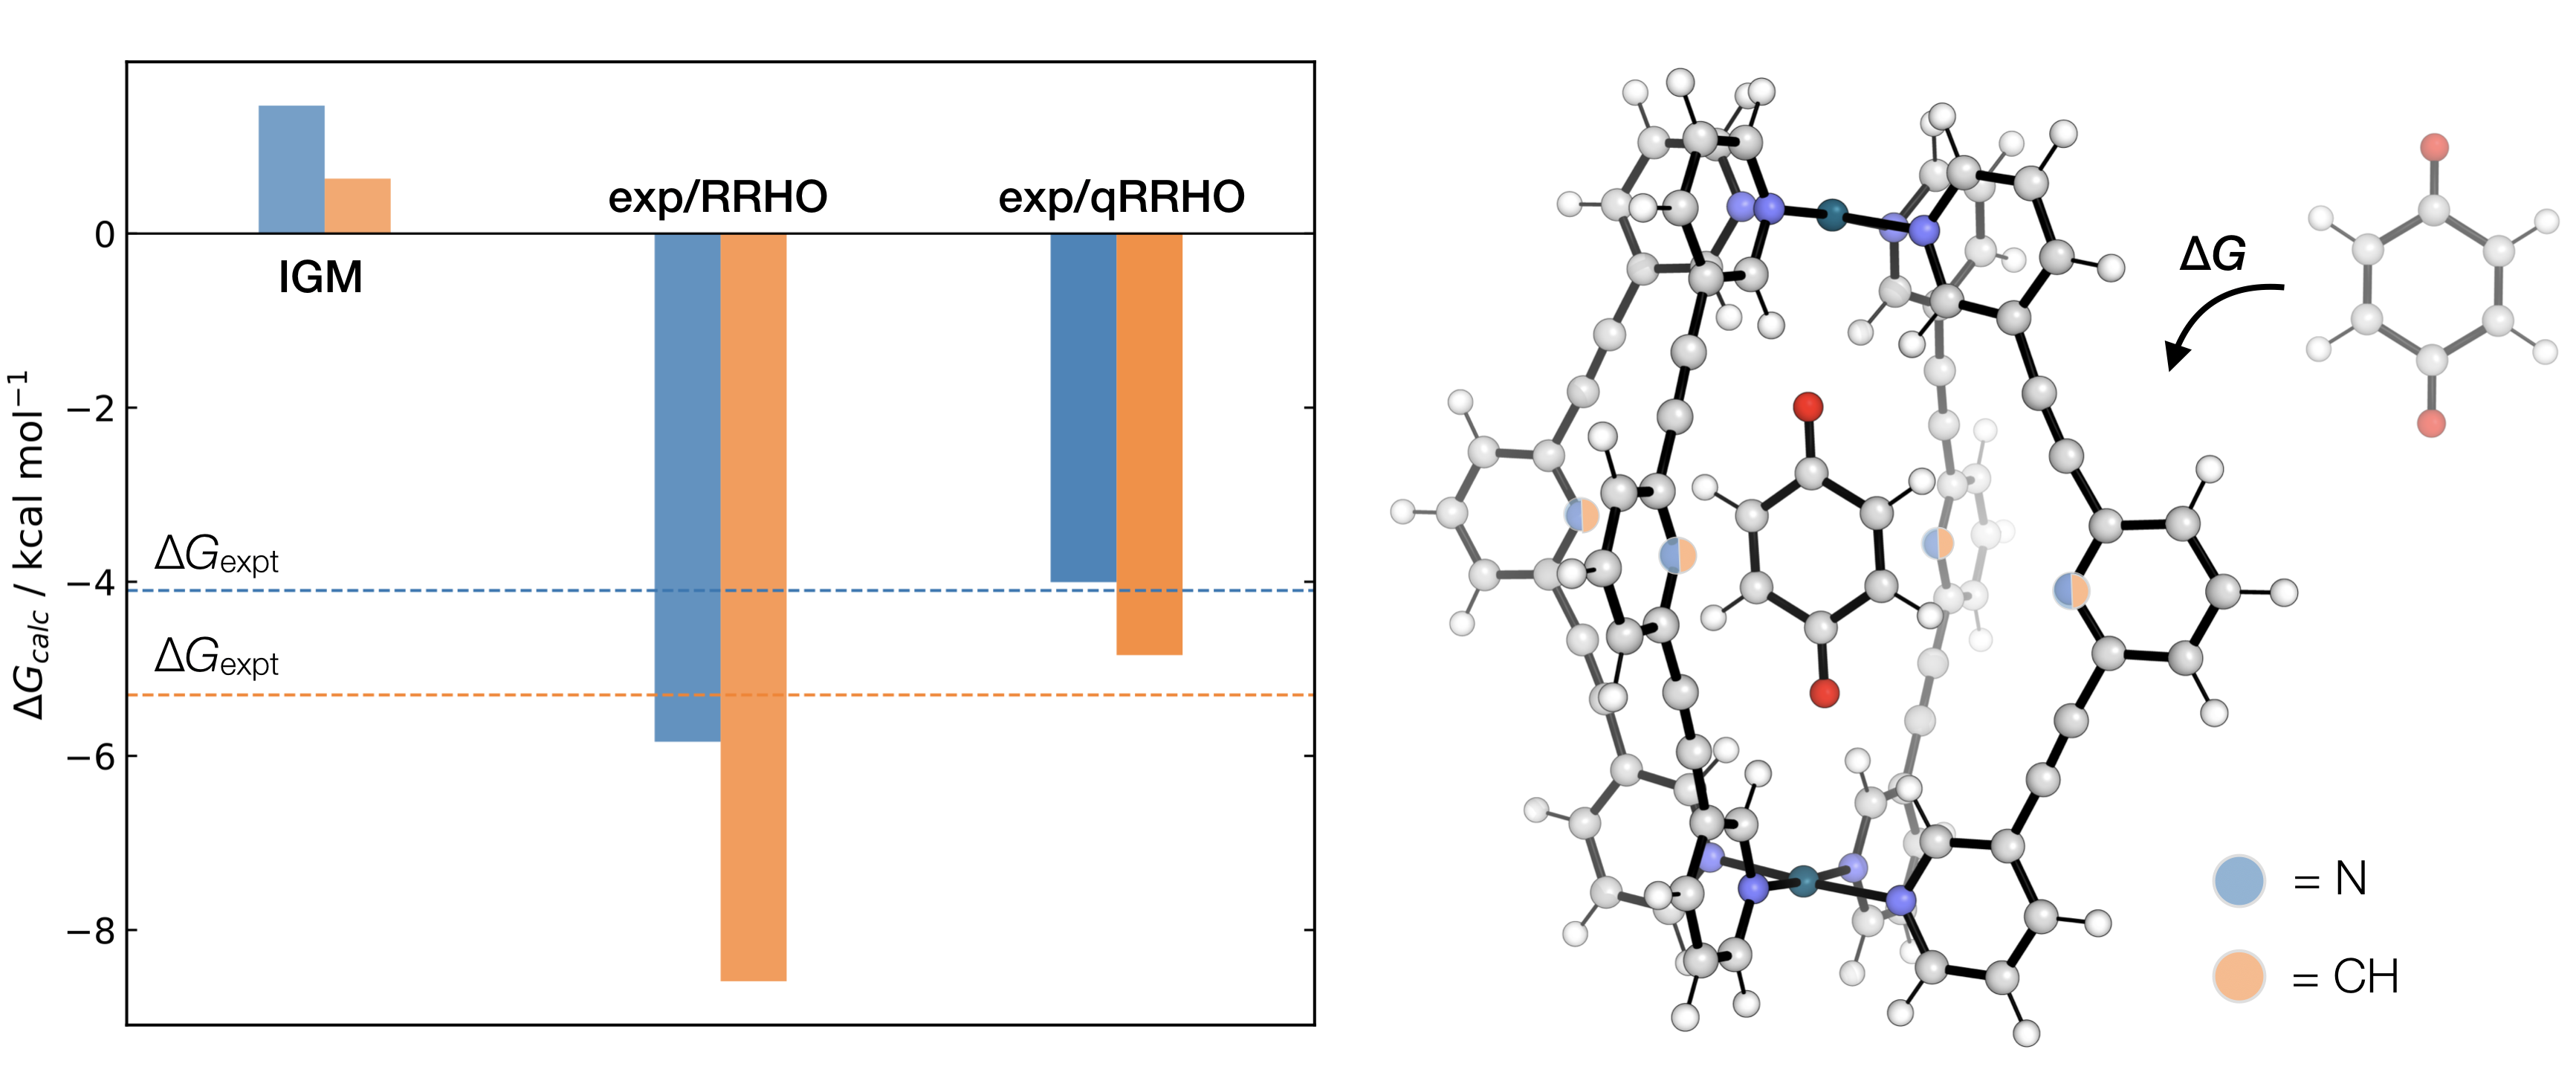
\includegraphics[width=\textwidth]{4/figs/figX12/figX12}
	\vspace{0.2cm}
	\hrule
	\caption{Comparison of free energy contributions added to SMD(DCM)/PBE0-D3BJ/gcp-def2-SVP binding energies for canonical benzoquinone binding within two [Pd$_2$L$_4$]${}^{2+}$ metallocages. IGM uses a PIB treatment of the translational entropy while exp uses an exponential well.} 
	\label{fig::entropy_X12}
\end{figure*}


\clearpage
\section{Conclusion}

The ideal gas model (IGM) has been implemented and used in quantum chemistry programs for the best part of 30 years with almost no development and, while successful for gas phase reactions, it remains suboptimal for the solution phase. The translational contribution to the entropy, which dominates the free energy cost of associating two molecules, uses a particle in an infinite cubic well approximation to calculate the partition function. Here, we have shown an exponential well (EW) can be used to evaluate the translational entropy more accurately, including the correct functional form and symmetry of the problem. The classical partition function and resulting entropy are easily obtainable from numerical integrals and, in general, converge to their quantum counterparts. 

However, with this treatment some limitations remain. Namely, (1) high-quality dynamics simulations are required to generate frames over which the EW is fit. This is partially alleviated by using an average model but introduces a $\sim 2$ \kcalx error. (2) The overestimation of the entropy lost by the IGM is often cancelled directly by the basis set superposition error (or dispersion overestimation). For example, in the water-in-water test case using uncorrected PBE0-D3BJ/def2-SVP free energies affords agreement largely within 1\kcalx to the true free energy difference. This observation hints to why the prototypical B3LYP/6-31G(d) method affords such good agreement to experimental free energies. (3) Perhaps most importantly, implicit solvent models that are generally (excluding non-polar solutes in non-polar solvents) important for accurate solution phase energetics implicitly include corrections for using the IGM in solution by their parametrisation to experiment.

In summary, while an EW approximation provides a more sound theoretical basis for translational motion in solution, it is unlikely to provide significant improvements over the IGM. A more effective approach to calculate accurate free energy differences is perhaps to use `free energy' methods in combination with fast, accurate and reactive potentials. Methods towards this latter strategy are developed in Chapter 6.

\section{Methods}

Density functional theory (DFT) and wave function (WF) calculations were performed in ORCA v. 4.2.1\cite{Neese2017} with Ahlrichs def2 basis sets\cite{Weigend2005}. DFT calculations used PBE0\cite{Adamo1999, Perdew1996} and M06-2X\cite{Zhao2007} density functional approximations with and without D3BJ\cite{Grimme2010, Grimme2011} damping respectively. Both DFT and WF (DLPNO-CCSD(T)\cite{Riplinger2013}) calculations made use of default auxiliary basis sets. Approximate counterpoise corrections performed using the gCP scheme from ref. \cite{Kruse2012} with parameters appropriate for the calculation. Fitted functions used \emph{scipy.optimise.curve\_fit}, numerical ordinary differential equation (ODE) propagation from  \emph{scipy.integrate.odeint} for toy models.\cite{SciPy} Converged partition functions obtained by summing partial eigenspecta located by root finding on numerically propagated ODEs using 4th order Runge Kutta\cite{Kutta1901} propagation implemented in \emph{odeint} from the \emph{Boost} C++ library.\cite{BoostODE2021} In all cases, numerical integration used \emph{scipy.integrate.quad} over a region that converges the integral with respect to the upper/lower bound (where infinite). Ideal gas and quasi-rigid rotor harmonic oscillator calculations performed in \emph{otherm}. Implicit solvent calculations made use of the CPCM\cite{Barone1998} and SMD\cite{Marenich2009} models implemented in ORCA while explicitly solvated calculations used MD simulations. Classical molecular mechanics MD performed in GROMACS v. 2019.2 using a minimise-equilibrate-production sequence.\cite{Abraham2015} Unless otherwise specified, all simulations were performed at 298.15 K using velocity rescale or Langevin thermostats. Periodic DFTB calculations performed with DFTB+\cite{Hourahine2020} using 3ob\cite{Gaus2012} parameters.

\clearpage
\end{document}